%!TEX encoding = UTF-8 Unicode
\documentclass[onecolumn,12pt]{book}
\usepackage[english,italian]{babel}
\usepackage{a4wide,Sweave,url}
\usepackage{verbatim}
\usepackage{makeidx}
\usepackage{babelbib}
\usepackage{float}
\usepackage{fancyhdr}
\usepackage[T1]{fontenc}
\usepackage[utf8]{inputenc}
\usepackage{framed}
\usepackage{lipsum}
\usepackage[dvipsnames]{color}
\definecolor{shadecolor}{rgb}{0.9,0.9,0.9}
\usepackage{graphicx}
\usepackage{fancyvrb}
\usepackage{amsmath}
\usepackage{Sweave}
\usepackage{hyperref}
\newenvironment{question}{\item \textbf{Esercizio}\newline}{}
\newenvironment{solution}{\textbf{Soluzione}\newline}{}
\newenvironment{answerlist}{\renewcommand{\labelenumi}{(\alph{enumi})}\begin{enumerate}}{\end{enumerate}}
\definecolor{grigetto}{rgb}{0.9,0.9,0.9}
 
\DefineVerbatimEnvironment{Sinput}{Verbatim} {xleftmargin=2em} \DefineVerbatimEnvironment{Soutput}{Verbatim}{xleftmargin=2em} \DefineVerbatimEnvironment{Scode}{Verbatim}{xleftmargin=2em} \fvset{listparameters={\setlength{\topsep}{0pt}}} \renewenvironment{Schunk}{\small\vspace{\topsep}}{\vspace{\topsep}\normalsize}
\lhead[\thepage]{\today}
%\usepackage{draftwatermark}
\usepackage{wrapfig}
\pagestyle{fancy}
\newcounter{fnotes}\setcounter{fnotes}{1}
\newcounter{Raction}\setcounter{Raction}{1}
\newcommand{\varia}[1]{\textsl{\textsf{#1}}}
\newcommand{\mytilde}{$\sim$}
\newcommand{\maurizio}[1]{\color{red}#1 \color{black}}
\newcommand{\federico}[1]{\color{green}#1 \color{black}}
 %\newenvironment{question}{\item \textbf{Problema}\newline}{}
%\newenvironment{solution}{\textbf{Soluzione}\newline}{}
%\DefineVerbatimEnvironment{Sinput}{Verbatim} {xleftmargin=2em,
                                            %  frame=single}
\DefineVerbatimEnvironment{Soutput}{Verbatim}{xleftmargin=2em,   frame=single}
 \newenvironment{ese} [1]{\vskip10pt
%\begin{center}
%\begin{minipage}{12cm}
 \markright{\today}
\definecolor{grigetto}{rgb}{0.9,0.9,0.9}
\colorbox{grigetto}{\parbox{\linewidth}{#1}}}
                          {
                         % \end{minipage}
                          %\end{center}
                          \medskip}
 \newcommand{\virgolette}{\selectlanguage{english}\texttt{"}\selectlanguage{italian}}
 \frontmatter\title{Matematica e Statistica con \textsf{R}}
\author{Federico Comoglio e  Maurizio Rinaldi}
\markright{\today}
\lhead{\today}
\renewcommand{\chaptermark}[1]{%
 \markboth{\chaptername
 \ \thechapter.\ #1}{}}
%\renewcommand{\sectionmark}[1]{%
% \markboth{\sectionname
% \ \thesection.\ #1}{}}
\newcommand{\rst}{\textsf{RStudio}~}
\newcommand{\rpr}{\textsf{R}~}
\makeindex
\begin{document}
\setkeys{Gin}{width=0.7\textwidth}
\Sconcordance{concordance:RbookParte2.tex:RbookParte2.Rnw:%
1 106 1 1 2 4 0 1 2 2 1 1 2 7 0 2 2 1 0 1 1 9 0 1 3 1 2 7 0 1 2 1 1 1 2 %
1 0 1 1 6 0 1 2 11 1 1 2 7 0 1 2 3 1 1 4 1 0 2 1 9 0 1 2 1 4 7 0 1 2 3 %
1 1 2 7 0 1 2 9 1 1 2 7 0 1 2 3 1 1 2 7 0 1 2 3 1 1 2 7 0 1 2 2 1 1 2 8 %
0 1 2 4 1 1 2 8 0 1 2 1 1 1 2 8 0 1 2 5 1 1 2 1 0 3 1 7 0 1 2 1 1 1 2 7 %
0 1 2 5 1 1 2 1 0 2 1 3 0 1 6 6 0 1 1 8 0 2 2 1 0 1 1 6 0 1 1 7 0 1 2 1 %
1 1 2 4 0 1 2 2 1 2 2 6 1 1 2 12 0 1 2 2 1 1 2 8 0 1 2 12 1 1 3 9 0 2 2 %
8 0 2 2 8 0 1 2 9 1 1 2 1 0 2 1 3 0 1 2 1 1 1 4 1 2 6 1 1 2 1 0 1 2 4 0 %
1 2 1 6 6 0 1 2 1 1 1 5 1 2 12 1 1 2 5 0 1 2 11 1 1 2 4 0 1 2 2 1 2 2 7 %
1 1 2 1 0 1 2 4 0 1 2 2 1 1 2 5 0 1 2 4 1 1 2 7 0 1 2 5 1 1 2 1 0 1 1 3 %
0 2 2 11 0 2 1 6 0 2 1 3 0 1 2 2 1 1 4 1 2 4 1 1 2 1 0 1 1 68 0 2 2 1 0 %
2 1 3 0 1 2 1 1 1 2 1 0 2 1 4 0 1 2 4 1 1 2 1 0 3 1 3 0 1 2 1 1 1 5 1 2 %
28 1 1 95 7 1 2 2 32 1 1 2 17 0 1 2 2 1 1 2 4 0 1 2 2 1 2 2 4 1 1 2 4 0 %
1 2 6 1 1 2 7 0 1 2 2 1 1 2 7 0 1 2 9 1 1 2 4 0 2 2 7 0 1 2 1 1 1 20 1 %
2 10 1 1 2 4 0 1 2 18 1 1 2 5 0 1 2 7 1 1 2 1 0 3 1 4 0 1 2 8 1 1 2 16 %
0 1 2 2 1 1 2 16 0 1 2 1 1 1 2 16 0 1 2 2 1 1 2 1 0 1 1 3 0 1 2 1 1 1 2 %
16 0 1 2 12 1 1 2 4 0 1 2 5 1 1 3 5 0 1 4 17 0 1 2 2 1 1 2 9 0 2 1 11 0 %
1 1 25 0 2 2 1 0 2 1 10 0 1 5 6 1 1 2 1 0 1 1 11 0 2 1 9 0 1 2 3 1 1 2 %
4 0 1 2 2 1 1 2 1 0 3 1 3 0 1 2 6 1 1 2 7 0 1 2 3 1 1 2 7 0 1 2 20 1 1 %
2 19 0 1 1 19 0 1 2 1 1 1 3 9 0 1 3 6 1 1 2 6 0 1 1 5 0 1 1 5 0 1 1 6 0 %
1 1 6 0 2 2 6 0 1 1 5 0 1 1 6 0 1 2 4 1 1 2 4 0 1 2 1 1 1 2 6 0 1 1 6 0 %
1 2 1 1 1 2 7 0 1 2 1 1 1 2 8 0 1 2 2 1 1 2 6 0 1 1 6 0 1 2 1 1 1 2 6 0 %
1 1 6 0 1 2 1 1 1 4 8 0 1 2 1 1 1 2 4 0 1 2 2 1 1 4 1 2 7 0 1 2 2 1 1 2 %
8 0 1 2 2 1 1 2 7 0 1 1 7 0 2 2 7 0 1 1 7 0 1 2 1 1 1 2 7 0 1 2 8 1 1 2 %
4 0 1 2 11 1 1 2 1 0 1 1 8 0 1 1 6 0 1 2 1 1 1 2 10 0 1 2 1 1 1 2 1 0 1 %
1 9 0 1 2 1 1 1 2 1 0 1 1 9 0 1 2 2 1 1 2 1 0 1 1 3 0 1 2 1 1 1 3 4 0 1 %
2 6 1 1 2 1 0 2 1 3 0 1 2 2 1 1 2 6 0 1 1 9 0 1 1 9 0 2 2 6 0 1 1 6 0 1 %
2 4 1 1 2 11 0 1 2 3 1 1 2 1 0 1 2 1 0 1 1 9 0 1 2 1 1 1 2 10 0 1 2 2 1 %
1 2 7 0 1 2 16 1 1 2 1 0 1 3 2 0 1 1 16 0 2 2 1 0 4 1 3 0 1 3 4 0 1 2 1 %
1 1 5 1 0 2 1 3 0 1 4 2 1 1 2 8 0 1 2 2 1 1 2 4 0 1 2 1 1 1 2 10 0 2 2 %
1 0 1 1 9 0 1 1 6 0 1 2 5 1 1 2 1 0 1 1 9 0 1 2 3 1 1 2 1 0 2 1 3 0 1 4 %
1 2 7 0 1 2 2 1 1 2 1 0 2 1 12 0 1 2 2 1 1 2 18 0 2 2 4 0 1 2 2 1 1 2 8 %
0 1 1 8 0 2 2 8 0 1 2 2 1 1 2 4 0 2 2 7 0 2 2 1 0 1 1 6 0 1 2 3 1 1 2 %
28 0 2 2 28 0 1 2 4 1 1 3 29 0 2 1 9 0 1 2 3 1 1 2 1 0 1 1 18 0 1 2 1 1 %
1 3 2 0 1 1 24 0 1 2 2 1 1 2 1 0 1 1 22 0 2 2 6 0 1 1 8 0 1 2 5 1 1 2 1 %
0 1 1 7 0 1 2 2 1 1 2 1 0 1 1 7 0 1 2 2 1 1 3 5 0 1 4 17 0 1 2 1 1 1 2 %
9 0 2 1 11 0 1 1 25 0 2 2 1 0 2 1 9 0 1 1 3 0 1 2 7 1 1 2 4 0 1 2 1 1 1 %
2 1 0 1 1 4 0 1 2 5 1 1 2 1 0 1 1 6 0 1 2 4 0 1 2 4 0 1 2 2 1 1 2 4 0 1 %
2 8 1 1 2 13 0 1 2 20 1 1 2 1 0 1 1 3 0 1 2 4 1 1 2 7 0 1 3 6 0 1 1 5 0 %
1 1 5 0 1 2 6 0 2 1 7 0 1 1 7 0 1 2 4 1 1 2 1 0 1 1 6 0 1 2 5 1 1 2 1 0 %
2 1 1 5 7 0 1 2 6 1 1 3 2 0 1 1 6 0 1 2 1 3 5 0 1 2 1 3 5 0 1 2 1 1 1 2 %
4 0 1 2 3 1 1 2 1 0 1 1 1 2 4 0 1 2 4 1 1 3 5 0 1 2 2 1 1 2 1 0 1 1 3 0 %
1 3 1 0 2 1 4 0 1 3 23 1 1 2 1 0 1 1 5 0 1 1 6 0 2 2 6 0 1 2 4 0 1 2 1 %
8 7 0 1 1 3 0 1 2 3 1 1 2 1 0 2 1 6 0 1 2 1 0 2 1 30 0 1 2 2 1 1 2 8 0 %
1 2 2 1 1 2 4 0 1 2 7 1 1 2 7 1 1 2 4 0 1 2 5 1 1 2 1 0 2 1 9 0 1 2 3 1 %
1 2 4 0 1 2 2 1 1 2 1 0 3 1 3 0 1 2 6 1 1 2 7 0 1 2 3 1 1 2 7 0 1 2 6 1 %
1 2 5 0 1 2 2 1 1 2 5 0 1 2 6 1 1 2 7 0 1 2 2 1 1 5 2 1 1 2 4 0 1 2 13 %
1 1 2 13 0 2 2 1 0 1 1 4 0 1 2 2 1 1 2 4 0 1 2 23 1 1 2 4 0 2 2 21 0 1 %
2 2 1 1 2 1 0 1 5 8 0 1 2 3 1 1 2 4 0 1 2 2 1 1 6 5 0 1 1 4 0 1 2 2 1 1 %
2 1 0 1 1 3 0 2 2 4 0 1 2 3 1 1 2 5 0 1 2 6 1 1 2 1 0 1 1 10 0 1 1 3 0 %
1 2 7 1 1 2 8 0 1 2 3 1 1 2 1 0 1 1 11 0 1 2 1 1 1 2 1 0 2 1 8 0 1 2 9 %
1 1 2 1 0 2 1 3 0 1 2 20 1 1 2 1 0 1 1 5 0 1 1 23 0 1 2 2 1 1 2 1 0 1 1 %
3 0 1 2 1 1 1 3 1 2 6 1 1 2 6 0 2 1 6 0 1 2 7 1 1 2 1 0 2 1 3 0 1 2 2 1 %
1 4 1 2 10 1 1 6 1 0 1 1 3 0 1 3 6 0 1 1 11 0 3 1 3 0 1 2 1 1 1 4 1 2 5 %
1 1 2 7 0 2 2 8 0 1 2 23 1 1 2 1 0 1 1 1 2 1 0 1 2 1 0 1 2 1 0 1 3 5 0 %
1 2 1 1 1 11 1 2 12 1 1 2 1 0 1 1 3 0 1 2 2 1 1 3 1 2 4 1 1 2 24 0 1 2 %
1 1 1 2 5 0 1 2 3 1 1 2 1 0 1 1 1 2 1 0 2 1 1 3 2 0 2 1 4 0 1 2 3 1 1 4 %
3 0 1 1 3 0 1 2 2 1 1 5 1 2 5 1 1 2 1 0 11 1 4 0 1 2 1 1 1 9 10 0 1 2 3 %
1 1 2 1 0 5 1 1 2 5 0 1 2 16 1 1 2 1 0 1 1 3 0 1 2 1 1 1 3 1 2 9 1 1 2 %
1 0 2 1 1 2 1 0 2 1 3 0 1 2 10 1 1 2 1 0 2 1 3 0 1 2 2 1 1 4 1 2 5 1 1 %
2 1 0 6 1 3 0 1 2 3 1 1 -11 1 0 6 1 1 8 5 1 4 0 1 2 1 1 1 2 1 0 6 1 4 0 %
1 2 6 1 1 2 1 0 1 1 1 9 12 0 1 2 2 1 1 2 1 0 10 1 1 2 1 0 1 2 1 0 1 1 1 %
2 4 0 1 2 2 1 1 19 1 2 9 1 1 2 1 0 4 1 1 2 1 0 1 2 1 0 1 1 1 2 1 0 1 2 %
1 0 1 3 2 0 2 1 4 0 1 2 7 1 1 2 4 0 2 2 4 0 1 2 4 0 1 2 17 1 1 2 1 0 6 %
1 3 0 1 2 8 1 1 2 1 0 2 1 3 0 1 2 10 1 1 2 1 0 6 1 3 0 1 2 9 1 1 2 1 0 %
11 1 3 0 1 2 11 1 1 2 1 0 1 1 3 0 1 2 1 1 1 2 1 0 2 1 1 2 4 0 1 2 5 1 1 %
2 1 0 4 1 4 0 1 2 13 1 1 2 1 0 5 1 4 0 1 2 6 1 1 2 1 0 2 1 1 3 2 0 1 1 %
3 0 1 2 13 1 1 2 1 0 1 1 1 4 3 0 1 1 3 0 1 2 9 1 1 2 1 0 1 1 1 3 2 0 1 %
1 7 0 1 2 10 1 1 2 1 0 2 1 7 0 1 2 11 1 1 2 1 0 3 1 7 0 1 2 12 1 1 2 1 %
0 1 1 4 0 1 3 1 1 1 2 1 0 1 2 1 0 1 1 3 0 1 2 1 1 1 2 1 0 2 1 3 0 1 2 1 %
1 1 2 4 0 1 2 3 1 1 2 1 0 1 2 1 0 1 1 3 0 1 2 9 1 1 4 1 0 1 1 1 6 9 0 1 %
2 7 1 1 2 3 1 1 4 6 0 1 2 7 1 1 2 1 0 6 1 4 0 2 2 1 0 26 1 4 0 1 2 7 1 %
1 2 4 0 1 2 1 1 1 2 1 0 3 1 4 0 1 2 3 1 1 2 1 0 5 1 1 2 1 0 3 1 3 0 1 2 %
1 1 1 2 1 0 4 1 1 2 1 0 1 1 1 2 1 0 2 1 3 0 1 2 1 1 1 2 1 0 4 1 1 2 1 0 %
1 1 1 2 1 0 2 1 3 0 1 2 2 1 1 2 1 0 5 1 1 2 1 0 1 1 1 2 1 0 3 1 1 3 2 0 %
1 1 3 0 1 2 6 1 1 4 54 0 1 2 4 1 1 2 56 0 1 2 5 1 1 2 55 0 1 2 4 1 1 2 %
107 0 1 3 5 1 1 2 104 0 1 2 20 1}

\markright{\today}
\thispagestyle{empty}
\maketitle
\newpage
\thispagestyle{empty}
\tableofcontents
\newpage
\thispagestyle{empty}
 \mainmatter

\chapter{Strutture di dati}
%\section{Aritmetica modulare}
 
Premettiamo che per visualizzare un oggetto di \textsf{R} si pu\`o usare il comando \texttt{print} o il comando \texttt{cat} che fornisce spesso un risultato migliore. \texttt{str} visualizza la struttura di un oggetto mentre \texttt{head} o \texttt{tail} ne visualizzano l'inizio o la fine.


\section{Le stringhe}
Una stringa\index{stringa} di testo \`e una collezione di caratteri; in genere, una stringa \`e resa riconoscibile dall'essere racchiusa tra virgolette.
\subsection{Operare con le stringhe}
Oltre alle virgolette, vi sono numerosi altri caratteri speciali che possono apparire in una stringa.
I pi\`u comuni sono ``\texttt{\textbackslash t}'' per \texttt{TAB}, `` \texttt{\textbackslash n}'' per una nuova linea e ``\texttt{\textbackslash }'' per un singolo {\it backslash}.
Quest'ultimo carattere \`e un carattere di \emph{escape} e consente una lettura diversa di quanto lo segue.  Per esempio
\begin{Schunk}
\begin{Sinput}
> cat("\"sin\"")
\end{Sinput}
\begin{Soutput}
"sin"
\end{Soutput}
\begin{Sinput}
> nchar("\"sin\"")
\end{Sinput}
\begin{Soutput}
[1] 5
\end{Soutput}
\begin{Sinput}
> cat("\\")
\end{Sinput}
\begin{Soutput}
\
\end{Soutput}
\begin{Sinput}
> cat("ora a capo\nsono a capo?")
\end{Sinput}
\begin{Soutput}
ora a capo
sono a capo?
\end{Soutput}
\begin{Sinput}
> cat("ora spazio\triprendo")
\end{Sinput}
\begin{Soutput}
ora spazio	riprendo
\end{Soutput}
\end{Schunk}
La funzione \texttt{nchar}, \index{\texttt{nchar}} che conta il numero di caratteri di una stringa, non includer\`a quindi il carattere di \emph{escape}\index{\emph{escape}} nel totale dei caratteri. Ad esempio:
\begin{Schunk}
\begin{Sinput}
> "Tab\t"
\end{Sinput}
\begin{Soutput}
[1] "Tab\t"
\end{Soutput}
\begin{Sinput}
> cat("Tab\t")
\end{Sinput}
\begin{Soutput}
Tab	
\end{Soutput}
\begin{Sinput}
> nchar("Tab\t")
\end{Sinput}
\begin{Soutput}
[1] 4
\end{Soutput}
\end{Schunk}



Succede spesso di dover lavorare in modo automatico con stringhe di testo, anche nello scrivere indirizzi di rete o cartelle di lavoro. In  \textsf{R} diversi comandi consentono la  generazione, manipolazione e stampa di una o pi\`u stringhe di testo\footnote{Per un  uso pi\`u specifico si pu\`o consultare il pacchetto \texttt{biostrings}.}. Consideriamo inizialmente una singola frase.
%codechunk
\begin{Schunk}
\begin{Sinput}
> x="lavorare con le stringhe"
\end{Sinput}
\end{Schunk}
Possiamo verificarne la classe e determinare il numero di caratteri di \texttt{x}
%codechunk
\begin{Schunk}
\begin{Sinput}
> class(x)
\end{Sinput}
\begin{Soutput}
[1] "character"
\end{Soutput}
\begin{Sinput}
> nchar(x)
\end{Sinput}
\begin{Soutput}
[1] 24
\end{Soutput}
\end{Schunk}
e anche considerare sottostringhe
%codechunk
\begin{Schunk}
\begin{Sinput}
> substr(x,3,8)
\end{Sinput}
\begin{Soutput}
[1] "vorare"
\end{Soutput}
\end{Schunk}
o  abbreviazioni ottenibili con il comando \texttt{abbreviate} \index{\texttt{abbreviate}}
%codechunk
\begin{Schunk}
\begin{Sinput}
> abbreviate("Mario Rossi",4)
\end{Sinput}
\begin{Soutput}
Mario Rossi 
     "MrRs" 
\end{Soutput}
\end{Schunk}

Certi oggetti possono essere convertiti a stringhe: per esempio il numero 2 pu\`o essere visto come una stringa e riconvertito a numero.
%codechunk
\begin{Schunk}
\begin{Sinput}
>  i=2;toString(i)
\end{Sinput}
\begin{Soutput}
[1] "2"
\end{Soutput}
\begin{Sinput}
> as.numeric(toString(i))
\end{Sinput}
\begin{Soutput}
[1] 2
\end{Soutput}
\end{Schunk}
Alcune stringhe molto frequenti sono le lettere \index{\texttt{letters}}\index{\texttt{LETTERS}} dell'alfabeto, maiuscole o minuscole
%codechunk
\begin{Schunk}
\begin{Sinput}
> letters[1:10]
\end{Sinput}
\begin{Soutput}
 [1] "a" "b" "c" "d" "e" "f" "g" "h" "i" "j"
\end{Soutput}
\begin{Sinput}
> LETTERS[1:10]
\end{Sinput}
\begin{Soutput}
 [1] "A" "B" "C" "D" "E" "F" "G" "H" "I" "J"
\end{Soutput}
\end{Schunk}
o i mesi dell'anno (per esempio abbreviati in inglese)\index{\texttt{month.abb}}
%codechunk
\begin{Schunk}
\begin{Sinput}
> month.abb
\end{Sinput}
\begin{Soutput}
 [1] "Jan" "Feb" "Mar" "Apr" "May" "Jun" "Jul" "Aug" "Sep"
[10] "Oct" "Nov" "Dec"
\end{Soutput}
\end{Schunk}
Le stringhe possono poi essere ``incollate'' con il comando\index{\texttt{paste}}
%codechunk
\begin{Schunk}
\begin{Sinput}
> paste("a","b",sep="")
\end{Sinput}
\end{Schunk}
dove \texttt{sep}  indica il separatore usato.
E tutto insieme
%codechunk

\begin{Schunk}
\begin{Sinput}
> for (i in 1:5) cat(paste("a",toString(i),"\t",sep=""))
\end{Sinput}
\begin{Soutput}
a1	a2	a3	a4	a5	
\end{Soutput}
\end{Schunk}
Il comando pu\`o anche essere utilizzato su vettori.
Per esempio
%codechunk
\begin{Schunk}
\begin{Sinput}
> paste(letters[1:10],1:10,sep="")
\end{Sinput}
\begin{Soutput}
 [1] "a1"  "b2"  "c3"  "d4"  "e5"  "f6"  "g7"  "h8"  "i9" 
[10] "j10"
\end{Soutput}
\end{Schunk}
La \textit{recycling rule} continua a valere
%codechunk

\begin{Schunk}
\begin{Sinput}
> paste(letters[1:3],1:10,sep="")
\end{Sinput}
\begin{Soutput}
 [1] "a1"  "b2"  "c3"  "a4"  "b5"  "c6"  "a7"  "b8"  "c9" 
[10] "a10"
\end{Soutput}
\begin{Sinput}
> paste(letters[1:3],1:12,sep="")
\end{Sinput}
\begin{Soutput}
 [1] "a1"  "b2"  "c3"  "a4"  "b5"  "c6"  "a7"  "b8"  "c9" 
[10] "a10" "b11" "c12"
\end{Soutput}
\end{Schunk}
e giocando con \texttt{rep} si possono ottenere diverse combinazioni.
\begin{Schunk}
\begin{Sinput}
> paste(rep(letters[1:3],each=5),1:15,sep="")
\end{Sinput}
\begin{Soutput}
 [1] "a1"  "a2"  "a3"  "a4"  "a5"  "b6"  "b7"  "b8"  "b9" 
[10] "b10" "c11" "c12" "c13" "c14" "c15"
\end{Soutput}
\begin{Sinput}
> paste(rep(letters[1:3],ntimes=5),1:15,sep="")
\end{Sinput}
\begin{Soutput}
 [1] "a1"  "b2"  "c3"  "a4"  "b5"  "c6"  "a7"  "b8"  "c9" 
[10] "a10" "b11" "c12" "a13" "b14" "c15"
\end{Soutput}
\end{Schunk}
Con l'opzione \texttt{collapse="x"} le stringhe vengono unite con separatore la stringa "x".
%codechunk
\begin{Schunk}
\begin{Sinput}
> paste(c("X", "Y"), 1:4, sep = "-", collapse = "--")
\end{Sinput}
\begin{Soutput}
[1] "X-1--Y-2--X-3--Y-4"
\end{Soutput}
\end{Schunk}
Si noti il separatore - dell'operazione \texttt{paste} e  - - dell'operazione \texttt{collapse}.

 \begin{shaded}
 \begin{enumerate}
 \item{} Inserisci il tuo cognome in una variabile `cognome' ed il tuo nome in una variabile 'nome'. Crea una terza variabile 'nomecognome' che contenga entrambi separati da un TAB. Stampa a console la scritta "Good job" seguita dal valore di nomecognome.
  \item{} Creare un elenco che contenga mesi e anno dal 2001 al 2010 nel seguente formato "tre lettere iniziali del mese-anno".
 \item{} Costruire una tabella che contenga tutte le parole di 2 lettere.
\item{}
Si consideri
\begin{Schunk}
\begin{Sinput}
> paste(letters[1:7],1:7,sep="=")
\end{Sinput}
\end{Schunk}
Estendere la corrispondenza a tutto l'alfabeto.
\item Creare un elenco in cui a ciascun mese corrisponda il suo numero (a partire da gennaio).
\item Creare un elenco con nomi i mesi e valori il numero di giorni di ciascun mese.
\item Scrivere un elenco di 5 persone con le relative date di nascita nel formato anno-mese-giorno.
 \end{enumerate}
 \end{shaded}

\section{Matrici}

Assegnati $n\times m$ ingressi possiamo costruire una matrice (ossia una tabella) con $n$ righe e $m$ colonne. Occorre solo riempire la matrice per righe o per colonne.
Ad esempio:
%code chunk
\begin{Schunk}
\begin{Sinput}
> a<-matrix(letters[1:12],nrow=3,ncol=4)
> a
\end{Sinput}
\begin{Soutput}
     [,1] [,2] [,3] [,4]
[1,] "a"  "d"  "g"  "j" 
[2,] "b"  "e"  "h"  "k" 
[3,] "c"  "f"  "i"  "l" 
\end{Soutput}
\begin{Sinput}
> class(a)
\end{Sinput}
\begin{Soutput}
[1] "matrix"
\end{Soutput}
\end{Schunk}
Se i parametri hanno natura diversa vengono resi uniformi
%code chunk
\begin{Schunk}
\begin{Sinput}
> a<-matrix(c(1:6,letters[1:6]),nrow=3,ncol=4);a
\end{Sinput}
\begin{Soutput}
     [,1] [,2] [,3] [,4]
[1,] "1"  "4"  "a"  "d" 
[2,] "2"  "5"  "b"  "e" 
[3,] "3"  "6"  "c"  "f" 
\end{Soutput}
\end{Schunk}
Con il parametro \texttt{byrow=T} il riempimento avviene per righe, anzich\`e per colonne.
%code chunk
\begin{Schunk}
\begin{Sinput}
>  a<-matrix(1:12,nrow=3,ncol=4,byrow=T)
>  a
\end{Sinput}
\begin{Soutput}
     [,1] [,2] [,3] [,4]
[1,]    1    2    3    4
[2,]    5    6    7    8
[3,]    9   10   11   12
\end{Soutput}
\end{Schunk}
Se i numeri sono insufficienti vengono \emph {riciclati}
%code chunk
\begin{Schunk}
\begin{Sinput}
> a<-matrix(1:4,nrow=3,ncol=4)
> a
\end{Sinput}
\begin{Soutput}
     [,1] [,2] [,3] [,4]
[1,]    1    4    3    2
[2,]    2    1    4    3
[3,]    3    2    1    4
\end{Soutput}
\end{Schunk}
in modo pacifico se sono un sottomultiplo della dimensione della matrice o con qualche
\texttt{warning} altrimenti.
%code chunk
\begin{Schunk}
\begin{Sinput}
> a<-matrix(2,nrow=3,ncol=4)
> a
\end{Sinput}
\end{Schunk}
Si possono anche definire gli ingressi attraverso opportune funzioni
%code chunk
\begin{Schunk}
\begin{Sinput}
> for(j in (1:4)) for(i in (1:3))  a[i,j]<-i^2+j
\end{Sinput}
\end{Schunk}
Per assegnare nomi alle  righe e alle colonne:\index{\texttt{colnames}} \index{\texttt{rownames}}
\begin{eqnarray*}
 \texttt{colnames}(\varia{matrice})=\texttt{c}(\virgolette \varia{  nome}_1\virgolette,\\
\virgolette \varia{nome}_2\virgolette,\ldots,\virgolette \varia{nome}_n\virgolette )\\
 \texttt{rownames}(\varia{matrice})=\texttt{c}(\virgolette \varia{nome}_1\virgolette,\\
\virgolette \varia{nome}_2\virgolette,\ldots,\virgolette \varia{nome}_n\virgolette )
\end{eqnarray*}
\begin{Schunk}
\begin{Sinput}
> colnames(a)=c("c1","c2","c3")
> rownames(a)=c("r1","r2","r3")
> a
\end{Sinput}
\end{Schunk}
\subsubsection{Aggiungere righe o colonne}
Per aggiungere una o pi\`u righe (o colonne)
ad una matrice si possono usare i comandi (\texttt{rbind} e \texttt{cbind})
\begin{Schunk}
\begin{Sinput}
> dim(a)
\end{Sinput}
\begin{Soutput}
[1] 3 4
\end{Soutput}
\begin{Sinput}
> rbind(a,letters[1:ncol(a)])
\end{Sinput}
\begin{Soutput}
     [,1] [,2] [,3] [,4]
[1,] "1"  "4"  "3"  "2" 
[2,] "2"  "1"  "4"  "3" 
[3,] "3"  "2"  "1"  "4" 
[4,] "a"  "b"  "c"  "d" 
\end{Soutput}
\begin{Sinput}
> cbind(a,letters[1:nrow(a)])
\end{Sinput}
\begin{Soutput}
     [,1] [,2] [,3] [,4] [,5]
[1,] "1"  "4"  "3"  "2"  "a" 
[2,] "2"  "1"  "4"  "3"  "b" 
[3,] "3"  "2"  "1"  "4"  "c" 
\end{Soutput}
\end{Schunk}
Possiamo anche effettuare semplici operazioni, come somma degli elementi delle righe o delle colonne
\begin{Schunk}
\begin{Sinput}
> colSums(a)
\end{Sinput}
\begin{Soutput}
[1] 6 7 8 9
\end{Soutput}
\begin{Sinput}
> rowSums(a)
\end{Sinput}
\begin{Soutput}
[1] 10 10 10
\end{Soutput}
\end{Schunk}

\subsection{Operazioni con le matrici}
\subsubsection{Trasposizione}
Per invertire righe e colonne di una matrice ossia per ottenere il trasposto \index{trasposto} di una matrice si usa il comando \texttt{t}(\texttt{matrice})\index{\texttt{t}, trasposto}
%code chunk
\begin{Schunk}
\begin{Sinput}
> t(a)
\end{Sinput}
\begin{Soutput}
     [,1] [,2] [,3]
[1,]    1    2    3
[2,]    4    1    2
[3,]    3    4    1
[4,]    2    3    4
\end{Soutput}
\end{Schunk}
\subsubsection{Prodotto}
Per la  moltiplicazione di matrici (definita per ingressi numerici) si usa il simbolo \texttt{\%*\%}.
\index{\texttt{\%*\%}, prodotto di matrici}
 %code chunk
\begin{Schunk}
\begin{Sinput}
> b<-matrix(2,nrow=3,ncol=3)
> for(j in (1:3))
+ for(i in (1:3)) b[i,j]<-i+j+i^2
> b
\end{Sinput}
\begin{Soutput}
     [,1] [,2] [,3]
[1,]    3    4    5
[2,]    7    8    9
[3,]   13   14   15
\end{Soutput}
\end{Schunk}
Non \`e infatti possibile moltiplicare una matrice 3x4 con una 3x3. Possiamo per\`o calcolare
%code chunk
\begin{Schunk}
\begin{Sinput}
> b%*%a
\end{Sinput}
\begin{Soutput}
     [,1] [,2] [,3] [,4]
[1,]   26   26   30   38
[2,]   50   54   62   74
[3,]   86   96  110  128
\end{Soutput}
\end{Schunk}
\subsubsection{Determinante} Il determinante di una matrice quadrata si ottiene con il comando
%\index{\texttt{det},determinante}
\begin{equation}\texttt{det} (\varia{matrice})\end{equation}
\begin{Schunk}
\begin{Sinput}
> det(b)
\end{Sinput}
\begin{Soutput}
[1] 1.887379e-14
\end{Soutput}
\end{Schunk}

Si noti che se eseguendo i calcoli a mano si trovano in alcuni casi risultati diversi da quelli di {\textsf R}. Per esempio la matrice in esame ha determinante 0 e 0 ne \`e anche un autovalore.\index{autovalore}
\begin{shaded}
 \begin{enumerate}
 \item{}Creare una matrice $3\times 2$ che abbia come ingressi i primi 6 numeri pari. Estendere la matrice aggiungendo due colonne contenenti i primi 6 numeri dispari. Calcolare e stampare la somma per riga e la somma per colonna. Modifica la matrice cambiando di segno la prima riga. Moltiplicare la matrice  per 4.
 \end{enumerate}
 \end{shaded}
 \section{I \emph{dataframe}}

I \emph{dataframe} (in \rpr  \texttt{data.frame}) costituiscono in \rpr la classe di oggetti fondamentali per la collezione di dati per una susseguente analisi statistica.
Un \emph{dataframe}  \`e una collezione di vettori aventi egual lunghezza e allineati verticalmente. Un dataframe \`e diverso da una matrice in quanto le colonne sono vettori eventualmente di tipi diversi. Il comando generale per costruire \emph{dataframe} a partire da vettori o liste
\`e \texttt{data.frame}.  Esso richiede come parametri i nomi dei vettori (colonna) da affiancare nella tabella. In generale si scrive:
\begin{equation*}\texttt{data.frame}(\varia{vettore}_1,\varia{vettore}_2, \ldots, \varia{vettore}_n)\end{equation*}
dove tutti i vettori hanno la stessa lunghezza.
Si noti la asimmetria  (rispetto ad una matrice) nel ruolo di righe e colonne. Le colonne sono omogenee, lo stesso non si pu\`o dire per le righe. Le colonne sono le variabili analizzate, le righe le unit\`a statistiche. Anche i vari comandi che vedremo rispettano tale differenza.
Il data.frame classico da cui partiamo è \texttt{iris}

Per avere una stampa abbreviata
%codechunk

\begin{Schunk}
\begin{Sinput}
> head(iris)
\end{Sinput}
\begin{Soutput}
  Sepal.Length Sepal.Width Petal.Length Petal.Width Species
1          5.1         3.5          1.4         0.2  setosa
2          4.9         3.0          1.4         0.2  setosa
3          4.7         3.2          1.3         0.2  setosa
4          4.6         3.1          1.5         0.2  setosa
5          5.0         3.6          1.4         0.2  setosa
6          5.4         3.9          1.7         0.4  setosa
\end{Soutput}
\begin{Sinput}
> tail(iris)
\end{Sinput}
\begin{Soutput}
    Sepal.Length Sepal.Width Petal.Length Petal.Width
145          6.7         3.3          5.7         2.5
146          6.7         3.0          5.2         2.3
147          6.3         2.5          5.0         1.9
148          6.5         3.0          5.2         2.0
149          6.2         3.4          5.4         2.3
150          5.9         3.0          5.1         1.8
      Species
145 virginica
146 virginica
147 virginica
148 virginica
149 virginica
150 virginica
\end{Soutput}
\end{Schunk}

Il comando \texttt{str}\index{\texttt{str}} consente una visualizzazione parziale che ci fornisce la struttura.
 
\small
\begin{Schunk}
\begin{Soutput}
'data.frame':	150 obs. of  5 variables:
 $ Sepal.Length: num  5.1 4.9 4.7 4.6 5 5.4 4.6 5 4.4 4.9 ...
 $ Sepal.Width : num  3.5 3 3.2 3.1 3.6 3.9 3.4 3.4 2.9 3.1 ...
 $ Petal.Length: num  1.4 1.4 1.3 1.5 1.4 1.7 1.4 1.5 1.4 1.5 ...
 $ Petal.Width : num  0.2 0.2 0.2 0.2 0.2 0.4 0.3 0.2 0.2 0.1 ...
 $ Species     : Factor w/ 3 levels "setosa","versicolor",..: 1 1 1 1 1 1 1 1 1 1 ...
\end{Soutput}
\end{Schunk}
\normalsize
Per esempio possiamo considerare il dataframe \texttt{d} definito come segue 
\begin{Schunk}
\begin{Sinput}
> L3 <- LETTERS[1:3]
> d <- data.frame(cbind(x=1, y=1:10,
+ fac=sample(L3, 10, replace=TRUE)),
+ stringsAsFactors=TRUE)
> d
\end{Sinput}
\begin{Soutput}
   x  y fac
1  1  1   A
2  1  2   B
3  1  3   C
4  1  4   B
5  1  5   C
6  1  6   B
7  1  7   B
8  1  8   B
9  1  9   B
10 1 10   B
\end{Soutput}
\end{Schunk}
Si noti che anche in questo caso si usa la \emph{recycling rule}
\begin{Schunk}
\begin{Sinput}
> data(crabs)
> dim(crabs)
\end{Sinput}
\begin{Soutput}
[1] 201   8
\end{Soutput}
\end{Schunk}
In quanto segue lavoreremo con il seguente \emph{dataframe} che rappresenta i risultati di un'indagine svolta sugli studenti che nell'Anno Accademico 2007/2008 frequentavano il primo anno del corso di Laurea di Farmacia della Facolt\`a di Farmacia del Piemonte Orientale. Potete scaricarlo dal sito e caricarlo in {\textsf R} con il comando
%code chunk
\begin{Schunk}
\begin{Sinput}
> data(farmacia)
\end{Sinput}
\end{Schunk}
Il comando \texttt{colnames}  consente di  visualizzare o assegnare il nome alle colonne.
Per esempio
%code chunk
\begin{Schunk}
\begin{Sinput}
> colnames(farmacia)
\end{Sinput}
\begin{Soutput}
[1] "Sex"  "W"    "H"    "Eyes" "Hair" "Sh"   "hM"  
[8] "hF"  
\end{Soutput}
\end{Schunk}
Le varie colonne hanno dei nomi di facile interpretazione. Si noti anche che a fianco di variabili numeriche (\texttt{W} e \texttt{H}, peso-altezza ad esempio) sono presenti variabili  \emph {nominali} quali sesso (\texttt{Sex}) e colore degli occhi (\texttt{Eyes}).
Per associare i nomi alle colonne  alle varie colonne dobbiamo eseguire una operazione di collegamento con il comando \texttt{attach},
%code chunk
\begin{Schunk}
\begin{Sinput}
> attach(farmacia)
\end{Sinput}
\end{Schunk}
A questo punto digitando il nome delle colonne appare il contenuto della colonna
%code chunk
\begin{Schunk}
\begin{Sinput}
> Sex
\end{Sinput}
\begin{Soutput}
 [1] F M M M F M F F M F F F F F M F F F M M M F F F F
[26] F M F M M F F M M F F F F M F M M F F F F F F F M
[51] M M F F M
Levels: F M
\end{Soutput}
\end{Schunk}
Le variabili nominali sono caratterizzate dal fatto che i loro valori (livelli, \texttt{levels}) \index{\texttt{level}} non hanno significato numerico, anche se possono essere codificati con dei numeri.   Ad esempio il sesso di una persona \`e una variabile nominale con due possibili valori, che sono stati  indicati qui con la convenzione  \texttt{"F"}  per le femmine e \texttt{"M"} per i maschi.  Se volessimo eliminare i livelli di una variabile nominale potremmo scrivere
\begin{Schunk}
\begin{Sinput}
> Sex=as.vector(Sex)
> Sex
\end{Sinput}
\begin{Soutput}
 [1] "F" "M" "M" "M" "F" "M" "F" "F" "M" "F" "F" "F"
[13] "F" "F" "M" "F" "F" "F" "M" "M" "M" "F" "F" "F"
[25] "F" "F" "M" "F" "M" "M" "F" "F" "M" "M" "F" "F"
[37] "F" "F" "M" "F" "M" "M" "F" "F" "F" "F" "F" "F"
[49] "F" "M" "M" "M" "F" "F" "M"
\end{Soutput}
\begin{Sinput}
> class(Sex)
\end{Sinput}
\begin{Soutput}
[1] "character"
\end{Soutput}
\end{Schunk}
Possiamo anche considerare il processo inverso e cambiare una variabile priva di livelli in una nominale
$$\texttt{factor}(\varia{variabile})\rightarrow\varia{ variabile}$$
Per definire i suoi livelli (ad esempio $n$) scriveremo:
$$\texttt{levels}(\varia{variabile})\leftarrow\texttt{c}(\varia{nome}_1,\varia{nome}_2,\ldots,\varia{nome}_n)$$
Per rendere la variabilie \texttt{Sex} nominale con nomi dei livelli
\texttt{F} e \texttt{M})  scriveremo:
\begin{Schunk}
\begin{Sinput}
> Sex=factor(Sex)
> Sex
\end{Sinput}
\begin{Soutput}
 [1] F M M M F M F F M F F F F F M F F F M M M F F F F
[26] F M F M M F F M M F F F F M F M M F F F F F F F M
[51] M M F F M
Levels: F M
\end{Soutput}
\end{Schunk}
Con il comando
\texttt{detach} \index{detach}  si pu\`o eliminare l'associazione creata tra colonne e nomi delle colonne.
Consideriamo ora un \emph{dataset} simile raccolto dagli studenti di Biotecnologie dello stesso anno
%code chunk
\begin{Schunk}
\begin{Sinput}
> sito="http://www.pharm.unipmn.it/rinaldi"
> nomefile="/file_corso/datibiotec.csv"
> biotec=read.table(paste(sito,nomefile,sep=""),sep=";",dec=",",header=T)
\end{Sinput}
\end{Schunk}
Scrivendo
\begin{Schunk}
\begin{Sinput}
> class(biotec)
\end{Sinput}
\begin{Soutput}
[1] "data.frame"
\end{Soutput}
\end{Schunk}
vediamo che anche \texttt{biotec} \`e un \emph{dataframe}.  Inoltre confrontando i nomi delle colonne di \texttt{farmacia} e di \texttt{biotec} possiamo verificare che sono essenzialmente uguali a meno di traduzione e eventuale abbreviazione.
Possiamo creare un \emph{dataframe} unico che raggruppi \texttt{biotec} e \texttt{farmacia}. Per farlo  vorremmo incollare un \emph{dataframe} sopra all'altro.
A tal fine occorre uniformare i nomi delle colonne scrivendo per esempio
\begin{Schunk}
\begin{Sinput}
> colnames(biotec)=colnames(farmacia)
> studenti=rbind(farmacia,biotec)
> head(studenti)
\end{Sinput}
\begin{Soutput}
  Sex  W    H     Eyes    Hair Sh   hM   hF
1   F 62 1.75  CASTANI CASTANI 40 1.77 1.78
2   M 64 1.84  CASTANI CASTANI 43 1.72 1.80
3   M 80 1.70  CASTANI CASTANI 44 1.65 1.73
4   M 80 1.75  CASTANI    NERI 44 1.66 1.78
5   F 50 1.70 NOCCIOLA    NERI 38 1.65 1.79
6   M 63 1.88  CASTANI  BIONDI 44 1.58 1.75
\end{Soutput}
\end{Schunk}
Si noti che il comando \texttt{rbind} \index{\texttt{rbind}} incolla per riga, mentre l'analogo comando \texttt{cbind}
\index{\texttt{cbind}} incolla le colonne.
Le intestazioni di riga di dati sono
\begin{Schunk}
\begin{Sinput}
> rownames(studenti)
\end{Sinput}
\begin{Soutput}
 [1] "1"   "2"   "3"   "4"   "5"   "6"   "7"  
 [8] "8"   "9"   "10"  "11"  "12"  "13"  "14" 
[15] "15"  "16"  "17"  "18"  "19"  "20"  "21" 
[22] "22"  "23"  "24"  "25"  "26"  "27"  "28" 
[29] "29"  "30"  "31"  "32"  "33"  "34"  "35" 
[36] "36"  "37"  "38"  "39"  "40"  "41"  "42" 
[43] "43"  "44"  "45"  "46"  "47"  "48"  "49" 
[50] "50"  "51"  "52"  "53"  "54"  "55"  "110"
[57] "210" "310" "410" "56"  "61"  "71"  "81" 
[64] "91"  "101" "111" "121" "131" "141" "151"
[71] "161" "171" "181" "191" "201" "211" "221"
[78] "231" "241" "251" "261" "271" "281" "291"
[85] "301" "311" "321" "331" "341" "351" "361"
[92] "371" "381" "391" "401" "411"
\end{Soutput}
\end{Schunk}
Per correggere la strana numerazione possiamo scrivere
\begin{Schunk}
\begin{Sinput}
> rownames(studenti)=seq(length=nrow(studenti))
\end{Sinput}
\end{Schunk}

Giunti a  questo punto la tabella \texttt{dati} presenta ancora alcuni problemi; per esempio se scriviamo
 %code chunk
\begin{Schunk}
\begin{Sinput}
> levels(studenti$Eyes)
\end{Sinput}
\begin{Soutput}
 [1] "AZZURRI"  "CASTANI"  "MARRONI"  "NERI"    
 [5] "NOCCIOLA" "VERDI"    "azzurri"  "castani" 
 [9] "marroni"  "verdi"   
\end{Soutput}
\begin{Sinput}
> levels(studenti$Hair)
\end{Sinput}
\begin{Soutput}
[1] "BIONDI"         "CASTANI"       
[3] "NERI"           "biondi"        
[5] "castani"        "castano chiaro"
[7] "castano scuro"  "neri"          
\end{Soutput}
\end{Schunk}
Ci incuriosisce   il dato con gli occhi neri. Verifichiamo:
\begin{Schunk}
\begin{Sinput}
> studenti[which(studenti$Eyes=="NERI"),]
\end{Sinput}
\begin{Soutput}
   Sex  W   H Eyes Hair Sh   hM   hF
20   M 69 1.7 NERI NERI 41 1.55 1.75
\end{Soutput}
\end{Schunk}
Possiamo ritenere che sia un errore e che in  realt\`a gli occhi siano marroni molto scuri.
Risulta evidente che nel riportare i colori degli  occhi si sono usate dizioni diverse per colori essenzialmente uguali, per esempio i livelli \texttt{"CASTANI"}, \texttt{"NOCCIOLA"},
\texttt{"MARRONI"} possono esser fatti confluire in un unico livello  \texttt{"castani"} e possiamo rendere minuscoli i nomi degli altri livelli con il comando
\begin{Schunk}
\begin{Sinput}
> options(width=50)
> levels(studenti$Eyes)=c("azzurri","castani","castani", "castani", "castani","verdi","azzurri","castani","castani","verdi")
\end{Sinput}
\end{Schunk}
A questo punto
\begin{Schunk}
\begin{Sinput}
> levels(studenti$Eyes)
\end{Sinput}
\begin{Soutput}
[1] "azzurri" "castani" "verdi"  
\end{Soutput}
\end{Schunk}
Facciamo lo stesso con i capelli
\begin{Schunk}
\begin{Sinput}
> levels(studenti$Hair)=c("biondi","castani","neri", "biondi", "castani","castani","castani","neri")
> levels(studenti$Hair)
\end{Sinput}
\begin{Soutput}
[1] "biondi"  "castani" "neri"   
\end{Soutput}
\end{Schunk}
\subsubsection{Selezione in base a criteri}
Supponiamo di voler selezionare gli studenti con gli occhi castani.
Basta scrivere
%code chunk
\begin{Schunk}
\begin{Sinput}
> subset(studenti,studenti$Eyes=="verdi")
\end{Sinput}
\begin{Soutput}
   Sex  W    H  Eyes    Hair Sh   hM   hF
7    F 63 1.70 verdi castani 38 1.72 1.82
17   F 51 1.55 verdi castani 37 1.60 1.70
25   F 91 1.81 verdi  biondi 42 1.60 1.87
33   M 75 1.82 verdi castani 43 1.60 1.75
35   F 46 1.64 verdi castani 37 1.56 1.89
37   F 56 1.70 verdi castani 39 1.68 1.90
38   F 55 1.65 verdi castani 38 1.68 1.70
41   M 56 1.70 verdi castani 39 1.65 1.80
42   M 67 1.73 verdi castani 42 1.55 1.85
47   F 52 1.75 verdi  biondi 38 1.62 1.80
51   M 75 1.76 verdi castani 42 1.60 1.68
58   M 64 1.74 verdi castani 41 1.63 1.80
60   M 64 1.80 verdi castani 42 1.56 1.75
72   F 55 1.67 verdi castani 40 1.60 1.80
76   M 85 1.84 verdi castani 43 1.69 1.69
77   F 60 1.67 verdi castani 38 1.64 1.70
81   F 62 1.61 verdi castani 39 1.60 1.66
90   F 49 1.60 verdi castani 40 1.58 1.75
91   F 62 1.76 verdi  biondi 40 1.70 1.73
93   F 53 1.65 verdi castani 38 1.55 1.85
95   M 80 1.80 verdi castani 44 1.68 1.70
\end{Soutput}
\end{Schunk}
Se siamo invece interessati al colore dei capelli degli studenti con occhi castani
\begin{Schunk}
\begin{Sinput}
> subset(studenti,studenti$Eyes=="verdi",select="Hair")
\end{Sinput}
\begin{Soutput}
      Hair
7  castani
17 castani
25  biondi
33 castani
35 castani
37 castani
38 castani
41 castani
42 castani
47  biondi
51 castani
58 castani
60 castani
72 castani
76 castani
77 castani
81 castani
90 castani
91  biondi
93 castani
95 castani
\end{Soutput}
\end{Schunk}


\section{Gli \emph{array}}
Un \emph{array}  \`e una generalizzazione multidimensionale di una matrice. Gli \emph{array} sono caratterizzati dal numero di dimensioni  (se le dimensioni sono 2 un \emph{array} si identifica con una  matrice) e dal nome dei vari livelli
%code chunk
\begin{Schunk}
\begin{Sinput}
> array(LETTERS[1:24],
+ dim=c(2,3,4))
\end{Sinput}
\begin{Soutput}
, , 1

     [,1] [,2] [,3]
[1,] "A"  "C"  "E" 
[2,] "B"  "D"  "F" 

, , 2

     [,1] [,2] [,3]
[1,] "G"  "I"  "K" 
[2,] "H"  "J"  "L" 

, , 3

     [,1] [,2] [,3]
[1,] "M"  "O"  "Q" 
[2,] "N"  "P"  "R" 

, , 4

     [,1] [,2] [,3]
[1,] "S"  "U"  "W" 
[2,] "T"  "V"  "X" 
\end{Soutput}
\begin{Sinput}
> array(sample(1:100,24), dim=c(3,4,2),dimnames=list(LETTERS[1:3],LETTERS[11:14],letters[1:2]))->x
> x[,,"b"]
\end{Sinput}
\begin{Soutput}
   K  L  M  N
A 60 77 15  6
B 31 26 64 88
C 37 68 87 18
\end{Soutput}
\end{Schunk}
\section{Liste}
Una lista (in \textsf{R} \texttt{list}) \`e un vettore di oggetti.  Gli oggetti possono avere un nome ed avere natura diversa fra di loro. \index{\texttt{list}}
Per esempio
%code chunk
\begin{Schunk}
\begin{Sinput}
> x=list(a=month.abb , b=array(rep(0,20), dim=c(4,5)),c="your name")
> x
\end{Sinput}
\begin{Soutput}
$a
 [1] "Jan" "Feb" "Mar" "Apr" "May" "Jun" "Jul"
 [8] "Aug" "Sep" "Oct" "Nov" "Dec"

$b
     [,1] [,2] [,3] [,4] [,5]
[1,]    0    0    0    0    0
[2,]    0    0    0    0    0
[3,]    0    0    0    0    0
[4,]    0    0    0    0    0

$c
[1] "your name"
\end{Soutput}
\end{Schunk}
Possiamo annidare anche liste entro liste
%code chunk
\begin{Schunk}
\begin{Sinput}
> x=list(a=1:10,b=array(rep(0,20),dim=c(4,5)),
+ c="testo",d=list(g="h",r=1:10) )
> x
\end{Sinput}
\begin{Soutput}
$a
 [1]  1  2  3  4  5  6  7  8  9 10

$b
     [,1] [,2] [,3] [,4] [,5]
[1,]    0    0    0    0    0
[2,]    0    0    0    0    0
[3,]    0    0    0    0    0
[4,]    0    0    0    0    0

$c
[1] "testo"

$d
$d$g
[1] "h"

$d$r
 [1]  1  2  3  4  5  6  7  8  9 10
\end{Soutput}
\end{Schunk}
\subsection{Funzioni applicate a oggetti}
\subsubsection{La funzione \texttt{apply}}
Quando abbiamo una struttura di dati a pi\`u dimensioni ad esempio un \emph{array}
\begin{Schunk}
\begin{Sinput}
> array(1:30,dim=c(2,5,3))->x
> x
\end{Sinput}
\begin{Soutput}
, , 1

     [,1] [,2] [,3] [,4] [,5]
[1,]    1    3    5    7    9
[2,]    2    4    6    8   10

, , 2

     [,1] [,2] [,3] [,4] [,5]
[1,]   11   13   15   17   19
[2,]   12   14   16   18   20

, , 3

     [,1] [,2] [,3] [,4] [,5]
[1,]   21   23   25   27   29
[2,]   22   24   26   28   30
\end{Soutput}
\end{Schunk}
possiamo applicare una funzione selezionando il livello escluso:
\begin{Schunk}
\begin{Sinput}
> apply(x,2,mean)
\end{Sinput}
\begin{Soutput}
[1] 11.5 13.5 15.5 17.5 19.5
\end{Soutput}
\begin{Sinput}
> apply(x,c(1,3),mean)
\end{Sinput}
\begin{Soutput}
     [,1] [,2] [,3]
[1,]    5   15   25
[2,]    6   16   26
\end{Soutput}
\end{Schunk}

In un \emph{dataframe} possiamo considerare diverse operazioni che coinvolgano due o pi\`u colonne. Per esempio possiamo considerare la tabella \texttt{farmacia} e proporci di calcolare la media del peso dei maschi e la media del peso delle femmine. Il comando \texttt{tapply} \index{\texttt{tapply}} consente di applicare una funzione ad una colonna di una tabella ripartita in gruppi in accordo ad un criterio specificato da un'altra colonna (nominale) della stessa tabella
\begin{eqnarray*}
\texttt{tapply}(\varia{vettore},\varia{criterio} ,\varia{funzione})\end{eqnarray*}
L'esempio sopra riportato si risolve con la scrittura:
%code chunk
\begin{Schunk}
\begin{Sinput}
> tapply(studenti$W, studenti$Sex,mean)->Wmean
> Wmean
\end{Sinput}
\begin{Soutput}
       F        M 
58.19298 69.34615 
\end{Soutput}
\end{Schunk}
Possiamo anche chiedere di calcolare altri indicatori sempre basandoci  su questa ripartizione maschi/femmine.
Ad esempio possiamo ottenere la deviazione standard(\texttt{sd}) di maschi e femmine:
%code chunk
\begin{Schunk}
\begin{Sinput}
> tapply(studenti$W, studenti$Sex,sd)->Wsd
> Wsd
\end{Sinput}
\begin{Soutput}
       F        M 
10.01149 10.61971 
\end{Soutput}
\end{Schunk}

\subsubsection{Il comando \texttt{table} applicato a diverse variabili nominali e le tabelle di contingenza}
Consideriamo il seguente \emph{dataframe} che riporta le ambizioni di un gruppo di scolari americani
\begin{Schunk}
\begin{Sinput}
> read.table("http://lib.stat.cmu.edu/DASL/Datafiles/PopularKids.html",
+ skip=39,header=T,nrow=478,sep="\t")->kidinterest
\end{Sinput}
\end{Schunk}
\begin{Schunk}
\begin{Soutput}
  Gender Grade Age  Race Urban.Rural School
1    boy     5  11 White       Rural    Elm
2    boy     5  10 White       Rural    Elm
3   girl     5  11 White       Rural    Elm
4   girl     5  11 White       Rural    Elm
5   girl     5  10 White       Rural    Elm
6   girl     5  11 White       Rural    Elm
    Goals Grades Sports Looks Money
1  Sports      1      2     4     3
2 Popular      2      1     4     3
3 Popular      4      3     1     2
4 Popular      2      3     4     1
5 Popular      4      2     1     3
6 Popular      4      2     1     3
\end{Soutput}
\end{Schunk}
Nella tabella le colonne che ci interessano al momento sono quelle che riguardano il sesso, gli obiettivi (scelti tra successo scolastico, capacit\`a sportiva e popolarit\`a) e la provenienza (colonne 1, 5  e 7). Nelle colonne dalla 8 alla 11 sono messi in ordine di importanza per il conseguimento della popolarit\`a  voti, sport, aspetto esteriore e denaro.
%codechunk
\begin{Schunk}
\begin{Sinput}
> colnames(kidinterest)
\end{Sinput}
\begin{Soutput}
 [1] "Gender"      "Grade"       "Age"        
 [4] "Race"        "Urban.Rural" "School"     
 [7] "Goals"       "Grades"      "Sports"     
[10] "Looks"       "Money"      
\end{Soutput}
\begin{Sinput}
> interessi=kidinterest[,c(1,5,7)]
> head(interessi)
\end{Sinput}
\begin{Soutput}
  Gender Urban.Rural   Goals
1    boy       Rural  Sports
2    boy       Rural Popular
3   girl       Rural Popular
4   girl       Rural Popular
5   girl       Rural Popular
6   girl       Rural Popular
\end{Soutput}
\begin{Sinput}
> table(interessi)
\end{Sinput}
\begin{Soutput}
, , Goals = Grades

      Urban.Rural
Gender Rural Suburban Urban
  boy     21       51    45
  girl    36       36    58

, , Goals = Popular

      Urban.Rural
Gender Rural Suburban Urban
  boy     19       20    11
  girl    31       22    38

, , Goals = Sports

      Urban.Rural
Gender Rural Suburban Urban
  boy     26       18    16
  girl    16        4    10
\end{Soutput}
\end{Schunk}
 Consideriamo per esempio le variabili provenienza e traguardi
\begin{Schunk}
\begin{Sinput}
> interessi2=kidinterest[,c(5,7)]
> tabella=table(interessi2)
> tabella
\end{Sinput}
\begin{Soutput}
           Goals
Urban.Rural Grades Popular Sports
   Rural        57      50     42
   Suburban     87      42     22
   Urban       103      49     26
\end{Soutput}
\end{Schunk}

La tabella di contingenza delle due variabili (in questo caso a 3  livelli ciascuna) si realizza con il comando
\texttt{table}.
\texttt{table}(\varia(lista))
applicato ad una singola variabile nominale conta le frequenze di ciascuna classe, se le variabili sono $n$ esamina tutte le combinazioni possibili ($2^n$ se le variabili sono dicotomiche) e ne conta tutte le occorrenze

Allo stesso modo possiamo creare una tabella dei colori degli occhi e dei capelli
%code chunk
\begin{Schunk}
\begin{Sinput}
> tabellaEH=table(studenti$Eyes,studenti$Hair)
\end{Sinput}
\end{Schunk}
 %code chunk
O ripartirne il peso in base al colore degli occhi
\begin{Schunk}
\begin{Sinput}
> stEyeW=split(studenti$W,studenti$Eyes)
> boxplot(stEyeW)
\end{Sinput}
\end{Schunk}
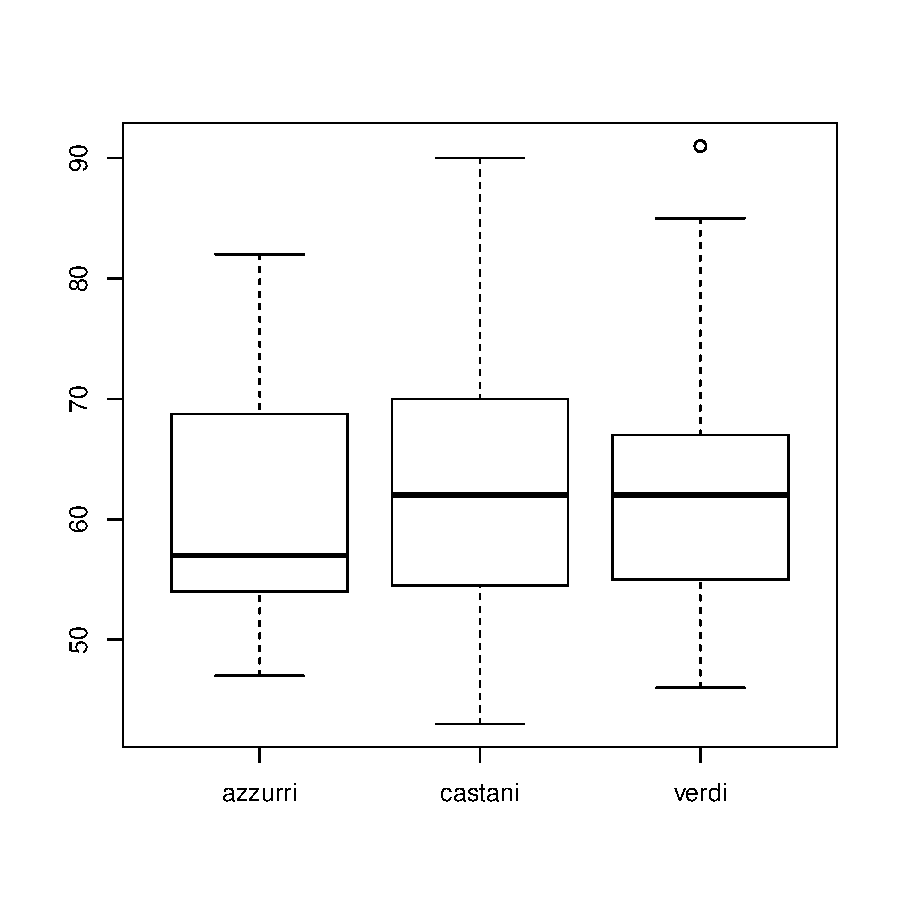
\includegraphics{RbookParte2-074}


\begin{enumerate}
\item{} Costruire una funzione \texttt{inserisci} tale che il comando
$\texttt{inserisci}(\varia{x}, \varia{dove},\varia{cosa})$ inserisca nel vettore $\varia{x}$ l'elemento $\varia{cosa}$ nella posizione $\varia{dove}$.
Per esempio
\begin{Schunk}
\begin{Sinput}
> y <-letters[1:10]
> y
\end{Sinput}
\begin{Soutput}
 [1] "a" "b" "c" "d" "e" "f" "g" "h" "i" "j"
\end{Soutput}
\end{Schunk}
\begin{Schunk}
\begin{Sinput}
> inserisci(x, 5, 0)
\end{Sinput}
\end{Schunk}
\begin{Schunk}
\begin{Soutput}
 [1] "a" "b" "c" "d" "0" "e" "f" "g" "h" "i" "j"
\end{Soutput}
\end{Schunk}
Generalizzare  al caso di inserimento di righe in \emph{dataframe}.
\item{}
Come si pu\`o verificare l'uguaglianza di 2 vettori includendo gli ingressi \texttt{NA}
\begin{Schunk}
\begin{Sinput}
> NA==NA
\end{Sinput}
\end{Schunk}
Aiuto: usare \texttt{is.na}
\item{}\cite{dalgaard}
Carichiamo il \emph{dataset} \texttt{juul} dal pacchetto \texttt{ISwR}. Ricavare il sottoinsieme di dati che corrispondono a ragazze tra i 7 e i 14 anni. Plottare \texttt{igf1} versus et\`a per ragazzi e ragazze separatamente. Conclusioni?
\end{enumerate}


\chapter{Operatori logici e selezione di elementi}
Consideriamo la selezione di elementi di un oggetto di \textsf{R}, per esempio \texttt{crabs}.
Selezioniamo per esempio tra i primi  50 i granchi con carapaci di lunghezza (sesta colonna) maggiore di 42:
\begin{Schunk}
\begin{Sinput}
> crabs[1:50,6]>42
\end{Sinput}
\begin{Soutput}
 [1] NA NA NA NA NA NA NA NA NA NA NA NA NA NA NA
[16] NA NA NA NA NA NA NA NA NA NA NA NA NA NA NA
[31] NA NA NA NA NA NA NA NA NA NA NA NA NA NA NA
[46] NA NA NA NA NA
\end{Soutput}
\end{Schunk}
Ciascun elemento del vettore viene confrontato con la soglia scelta (42) e quando supera la soglia la risposta \`e \texttt{TRUE} altrimenti \texttt{FALSE}.
\vskip20pt
%\begin{table}
\begin{tabular}
{|r r |}\hline
 \texttt{operatore}&  significato\\
\hline
\texttt{$>$}&  maggiore\\
\texttt{>=}& maggiore o uguale\\
\texttt{<}&   minore\\
\texttt{<=}&   minore o uguale\\
\texttt{==}&   uguale\\
\texttt{!=}&   diverso\\
\texttt{\&}&   and (e)\\
\texttt{|} & or (o)\\
\hline
\end{tabular}
\vskip20pt
%\end{table}
Gli ultimi due operatori combinano gli operatori precedenti. Per esempio
%code chunk
\begin{Schunk}
\begin{Sinput}
> crabs[crabs$sex == "F" | crabs$sp == "O",]
> dim(crabs[crabs$sex == "F" & crabs$sp == "O",])
\end{Sinput}
\end{Schunk}
%code chunk

\subsection{I valori non assegnati}
Capita frequentemente che un oggetto contenga valori non assegnati.
Per esempio
\begin{Schunk}
\begin{Sinput}
> x=1;x[10]=4;x
\end{Sinput}
\begin{Soutput}
 [1]  1 NA NA NA NA NA NA NA NA  4
\end{Soutput}
\end{Schunk}
\begin{Schunk}
\begin{Sinput}
> x[!is.na(x)]
\end{Sinput}
\begin{Soutput}
[1] 1 4
\end{Soutput}
\begin{Sinput}
> class(x)
\end{Sinput}
\begin{Soutput}
[1] "numeric"
\end{Soutput}
\begin{Sinput}
> class(unclass(x))
\end{Sinput}
\begin{Soutput}
[1] "numeric"
\end{Soutput}
\begin{Sinput}
> is.na(x)
\end{Sinput}
\begin{Soutput}
 [1] FALSE  TRUE  TRUE  TRUE  TRUE  TRUE  TRUE
 [8]  TRUE  TRUE FALSE
\end{Soutput}
\begin{Sinput}
>  DF <- data.frame(x = c(1, 2, 3), y = c(0, 10, NA))
> na.omit(DF)
\end{Sinput}
\begin{Soutput}
  x  y
1 1  0
2 2 10
\end{Soutput}
\begin{Sinput}
> complete.cases(x)
\end{Sinput}
\begin{Soutput}
 [1]  TRUE FALSE FALSE FALSE FALSE FALSE FALSE
 [8] FALSE FALSE  TRUE
\end{Soutput}
\end{Schunk}
\chapter{Statistica con \textsf{R}}
\section{Variabili aleatorie}
Una variabile aleatoria (\emph{random variabile}) \`e
 una variabile i cui valori sono soggetti a variazioni casuali. Quando i valori possibili di una variabile aleatoria  possono essere elencati parliamo di variabile aleatoria discreta. Quando i valori non possono essere elencati parliamo di variabile aleatoria continua.

\section{Variabili aleatorie discrete}
Le variabili aleatorie  discrete che  assumono un numero limitato di valori si dicono anche \emph{finite}.  I valori di una variabile aleatoria discreta possono essere numerici o nominali.
 Supponiamo di avere una variabile aleatoria che possa assumere un insieme di valori in  un \emph{alfabeto} assegnato costituito da lettere, parole o numeri. Per esempio un alfabeto pu\`o essere del tipo che segue
\begin{itemize}
\item{}(Femmina, Maschio)
\item{}(A,C,T,G)
\item{} (0,1)
\item{}(Ottimo, Buono, Discreto, Sufficiente, Insufficiente)
\item{} (Testa, Croce).
\item{} I numeri interi
\end{itemize}
Per caratterizzare completamente una variabile aleatoria discreta oltre ai valori che questa pu\`o  assumere occorre conoscere la probabilit\`a  di questi valori.


Per semplicit\`a considereremo variabili aleatorie finite.\\
Come possiamo simulare variabili aventi valore nell'alfabeto assegnato?
In effetti qualunque comando di generazione su un computer non \`e perfettamente casuale; infatti la generazione avviene in effetti in modo pseudo-casuale e  secondo un meccanismo che dipende dallo stato interno del computer codificato in una variabile indicata con \texttt{.Random.seed}. Se il {\it seme} iniziale \`e lo stesso i numeri generati saranno uguali. Spesso conviene che i calcoli (ad esempio a fine didattico) siano riproducibili. Ad esempio mettendo in una variabile \texttt{seme} il valore corrente di \texttt{.Random.seed} e richiamandolo o generandolo all'occorrenza.  
Un altro modo di procedere consiste nell'impostare il valore di 
\texttt{.Random.seed} attraverso il comando 
\texttt{set.seed}  la cui sintassi \`e 
$\texttt{set.seed}(\varia{n})$ dove $n$ \`e un numero intero.
 
\begin{Schunk}
\begin{Sinput}
> set.seed(3)
\end{Sinput}
\end{Schunk}
 
A questo punto possiamo simulare le variabili richieste usando la struttura
\begin{equation}\texttt{sample}(\varia{alfabeto},\varia{n})\end{equation}
Se l'alfabeto consiste di tutte le lettere minuscole dell'alfabeto ordinario e ne vogliamo selezionare $n=8$  (in modo che ciascun uscita abbia la stessa probabilit\`a)  basta scrivere
\begin{Schunk}
\begin{Sinput}
> sample(letters,8)
\end{Sinput}
\begin{Soutput}
[1] "e" "u" "j" "h" "n" "m" "c" "f"
\end{Soutput}
\end{Schunk}
Se invece l'alfabeto consiste delle basi del DNA
\begin{Schunk}
\begin{Sinput}
> alfabeto=c("A","C","G","T")
> sample(alfabeto,2)
\end{Sinput}
\begin{Soutput}
[1] "G" "C"
\end{Soutput}
\end{Schunk}
Notiamo che
\begin{Schunk}
\begin{Sinput}
>  sample(alfabeto)
\end{Sinput}
\begin{Soutput}
[1] "G" "C" "T" "A"
\end{Soutput}
\end{Schunk}
restituisce una permutazione dell'alfabeto, mentre chiedendo un campione di lunghezza superiore alla lunghezza dell'alfabeto otteniamo un messaggio di errore. Possiamo per\`o immaginare di re-immettere la lettera estratta nell'urna dopo ogni estrazione. In questo caso non c'\`e limite alla sequenza generata.
Per esempio
\begin{Schunk}
\begin{Sinput}
> alfabeto=c("testa","croce")
> sample(alfabeto,5,replace=T)
\end{Sinput}
\begin{Soutput}
[1] "croce" "croce" "testa" "croce" "croce"
\end{Soutput}
\end{Schunk}
 

Il precursore  del dado era chiamato astragalo ed era giocato nell'antica Grecia e nell'antica Roma~\cite{david}.
Gli  astragali sono dei piccoli ossicini di forma irregolare ed hanno 6 facce ma atterranno in  modo stabile solo su 4 di esse numerate 1, 3, 4 e 6  con probabilit\`a all'incirca 0.4 per il 3 e il 4  e di 0.1 per l'1 e il 6. In altre parole l'astragalo \`e descritto dalla tabella

\begin{center}\begin{tabular}{|r|r |}
\hline
 valore&  probabilit\`a \\
\hline
1&0.1\\
3 &0.4\\
4& 0.4\\
6&0.1\\
 \hline
\end{tabular}
\end{center}
Il tiro pi\`u gettonato all'epoca era l'uscita di 4 facce diverse nel lancio di 4 astragali e si chiamava {\it Venus}.
Il lancio considerato peggiore sul singolo lancio era l'1 chiamato cane o avvoltoio.
\begin{figure}[htbp]
\begin{center}
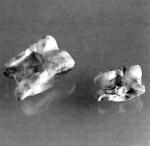
\includegraphics[width=6cm]{../grafici/astragals.jpeg}
\caption{ Astragalo. }
\label{fig:astragalo}
\end{center}
\end{figure}
Per simulare un astragalo su un computer
\begin{Schunk}
\begin{Sinput}
> sample(c(1,3,4,6),4,replace=T,prob=c(0.1,0.4,0.4,0.1))
\end{Sinput}
\begin{Soutput}
[1] 3 3 3 3
\end{Soutput}
\end{Schunk}

Torniamo ora ai classici dadi a 6 facce.
Supponiamo di lanciare 100 volte un dado equo a 6 facce e di registrare in \texttt{x}
le uscite rilevate
\begin{Schunk}
\begin{Sinput}
> set.seed(3)
> dadi100<-sample(1:6,100,replace=T)
> dadi100
\end{Sinput}
\begin{Soutput}
  [1] 2 5 3 2 4 4 1 2 4 4 4 4 4 4 6 5 1 5 6 2 2 1 1 1 2 5 4 6
 [29] 4 5 3 3 2 3 2 3 6 2 4 2 2 5 2 4 3 2 1 1 2 5 2 2 6 6 6 6
 [57] 3 2 1 2 5 1 5 1 5 2 5 4 3 1 5 5 6 6 4 4 1 1 5 5 5 4 3 1
 [85] 6 6 2 3 4 6 1 2 3 5 6 2 2 2 2 5
\end{Soutput}
\end{Schunk}
Volendo invece simulare una combinazione da giocare al SuperEnalotto possiamo scrivere
\begin{Schunk}
\begin{Sinput}
> (x<-sample(1:90,6,replace=T))
\end{Sinput}
\begin{Soutput}
[1] 69 62 19 65 55 31
\end{Soutput}
\end{Schunk}
I numeri usciti sono stati salvati  in una variabile \texttt{x}, per poter effettuare la ricerca di indicatori statistici.
Il comando che consente di ordinare una lista o un vettore \`e \texttt{sort}, esso pu\`o essere usato in associazione al nome di una variabile o di una lista, ossia:
\begin{equation}\texttt{sort}(\varia{variabile/lista})\end{equation}
Volendo ordinare i numeri precedentemente ricavati scriveremo
\begin{Schunk}
\begin{Sinput}
> sort(x)
\end{Sinput}
\begin{Soutput}
[1] 19 31 55 62 65 69
\end{Soutput}
\end{Schunk}



\section{Statistica descrittiva: singola variabile}
\subsection{Indicatori statistici}
\begin{itemize}
\item{}Media.\vskip0pt
La media di una serie di numeri si ottiene con la funzione \texttt{mean} scrivendo:
$\texttt{mean}(\varia{variabile})$.
Ad esempio, lavorando con la lunghezza del sepalo di 150 piante di iris
\begin{Schunk}
\begin{Sinput}
> x=iris[,1]
> mean(x)
\end{Sinput}
\begin{Soutput}
[1] 5.843333
\end{Soutput}
\end{Schunk}
\item{}Varianza campionaria\vskip0pt
Si ottiene con la funzione predefinita di espressione:
\texttt{var}(\varia{variabile}).
Possiamo calcolare la varianza come
\begin{Schunk}
\begin{Sinput}
> var(x)
\end{Sinput}
\begin{Soutput}
[1] 0.6856935
\end{Soutput}
\end{Schunk}
\item{}Deviazione Standard campionaria.\vskip0pt
Non \`e altro che la radice della varianza. Si ottiene con la funzione predefinita di espressione:
$\texttt{sd}(\varia{variabile})$.
Sempre basandosi sull'esempio precedente scriveremo
\begin{Schunk}
\begin{Sinput}
> sd(x)
\end{Sinput}
\begin{Soutput}
[1] 0.8280661
\end{Soutput}
\end{Schunk}

\item{}Quantili. La notazione standard \`e semplicemente: \texttt{quantile}(\varia{variabile}) che determina i quartili e ci fornisce in uscita la statistica dei 5 numeri

\begin{Schunk}
\begin{Sinput}
> quantile(x)
\end{Sinput}
\begin{Soutput}
  0%  25%  50%  75% 100% 
 4.3  5.1  5.8  6.4  7.9 
\end{Soutput}
\end{Schunk}
Volendo ricavare i decili dovremo scrivere:
$$\texttt{quantile}(\varia{variabile},\texttt{seq(0,1,by=0.1)})$$
in quanto vogliamo dividere l'intervallo $[0,1]$ a passo $0.1$

Nell'esempio:
\begin{Schunk}
\begin{Sinput}
> quantile(x,seq(0,1,by=0.1))
\end{Sinput}
\begin{Soutput}
  0%  10%  20%  30%  40%  50%  60%  70%  80%  90% 100% 
4.30 4.80 5.00 5.27 5.60 5.80 6.10 6.30 6.52 6.90 7.90 
\end{Soutput}
\end{Schunk}
Si noti che \texttt{quantile} ammette 9 varianti specificabili con l'opzione $\texttt{type}=n$ dove $n$ va da 1 a 9.
Per esempio
\begin{Schunk}
\begin{Sinput}
> quantile(x,type=2)
\end{Sinput}
\begin{Soutput}
  0%  25%  50%  75% 100% 
 4.3  5.1  5.8  6.4  7.9 
\end{Soutput}
\end{Schunk}
Sui dati in esame le 9 varianti coincidono. La convenzione da noi adottata corrisponde al numero 2
\end{itemize}
Per quanto riguarda gli indicatori statistici nel caso di dati ripetuti basta notare che se la lista $x$ contiene i valori e la lista $f$ le frequenze assolute il comando
$$\varia{rep}(x,f)$$ costruisce un'unica lista dei dati inclusiva delle ripetizioni.
Per esempio

\begin{Schunk}
\begin{Sinput}
> x=1:6
> f=c(9,7,9,7,8,10)
> (dati=rep(x,f))
\end{Sinput}
\begin{Soutput}
 [1] 1 1 1 1 1 1 1 1 1 2 2 2 2 2 2 2 3 3 3 3 3 3 3 3 3 4 4 4 4 4
[31] 4 4 5 5 5 5 5 5 5 5 6 6 6 6 6 6 6 6 6 6
\end{Soutput}
\end{Schunk}
Ovviamente senza bisogno di visualizzare \texttt{dati} possiamo calcolarne tutti gli indicatori statistici.
Il comando
\begin{Schunk}
\begin{Sinput}
> cumsum(f)
\end{Sinput}
\begin{Soutput}
[1]  9 16 25 32 40 50
\end{Soutput}
\end{Schunk}
restituisce le frequenze cumulate, dalle quali si possono ricavare facilmente la mediana
i quantili.

\subsection{Raggruppamenti in classi}
Consideriamo la rilevazione della temperatura media giornaliera di Milano nel mese di Gennaio 2016.
Scegliamo il mese
\begin{Schunk}
\begin{Soutput}
> stringa="Milano/2016/Gennaio?format=csv"
\end{Soutput}
\end{Schunk}
\begin{Schunk}
\begin{Sinput}
> sito="http://www.ilmeteo.it/portale/archivio-meteo/"
> indirizzo=paste(sito,stringa,sep="")
> meteo=read.table(indirizzo,sep=";",header=T)
\end{Sinput}
\end{Schunk}
\begin{Schunk}
\begin{Sinput}
> meteo
\end{Sinput}
\begin{Soutput}
   LOCALITA      DATA TMEDIA..C TMIN..C TMAX..C PUNTORUGIADA..C
1    Milano  1/1/2016         1      -2       4               1
2    Milano  2/1/2016         1       0       2               1
3    Milano  3/1/2016         1       0       3               1
4    Milano  4/1/2016         2       1       3               1
5    Milano  5/1/2016         3       2       5               2
6    Milano  6/1/2016         5       3       8               2
7    Milano  7/1/2016         3      -1       6               2
8    Milano  8/1/2016         2      -1       5               2
9    Milano  9/1/2016         5       3       5               4
10   Milano 10/1/2016         5       4       7               5
11   Milano 11/1/2016         6       4       8               6
12   Milano 12/1/2016         5       0      12               3
13   Milano 13/1/2016         7       1      12               0
14   Milano 14/1/2016         2      -2       5               1
15   Milano 15/1/2016         5       1      11               1
16   Milano 16/1/2016         5      -3      11               0
17   Milano 17/1/2016         6       2       8               0
18   Milano 18/1/2016         0      -5       5               0
19   Milano 19/1/2016        -1      -5       4               0
20   Milano 20/1/2016         0      -4       4               0
21   Milano 21/1/2016         0      -5       5               0
22   Milano 22/1/2016         0      -5       6               0
23   Milano 23/1/2016         2      -3       8               0
24   Milano 24/1/2016         2      -4       8               0
25   Milano 25/1/2016         4      -2      13               2
26   Milano 26/1/2016         7      -1      15               5
27   Milano 27/1/2016         7       1      12               5
28   Milano 28/1/2016         9       7      12               6
29   Milano 29/1/2016        10       6      15               6
30   Milano 30/1/2016         8       7       9               6
31   Milano 31/1/2016         8       4      13               7
   UMIDITA.. VISIBILITA.km VENTOMEDIA.km.h VENTOMAX.km.h
1         97             2               6            11
2         97             2               5             9
3         96             3               7            11
4         93             4               7            11
5         89             5               6            11
6         85             5               8            13
7         88             8               5            11
8         89             7               7            17
9         95             2               6            11
10        95             3               5            11
11        95             3               8            13
12        80             6               7            20
13        46            31              11            19
14        74            10               7            15
15        54             9              11            22
16        43            13              10            24
17        22            18              17            28
18        40            26               4            11
19        55            14               4             9
20        63            10               6            13
21        69             7               6            11
22        75             7               4             7
23        73             6               6            15
24        75             5               6            11
25        77             5               5            13
26        81             5               5            11
27        85             4               4             7
28        84             4               5             9
29        81             5               5            11
30        91             2               4             9
31        92             2               8            17
   RAFFICA.km.h PRESSIONESLM.mb PRESSIONEMEDIA.mb PIOGGIA.mm
1             0            1026                 0          0
2             0            1019                 0          0
3             0            1010                 0          0
4             0            1000                 0          0
5             0            1001                 0          0
6             0            1001                 0          0
7             0            1004                 0          0
8             0            1009                 0          0
9             0            1008                 0          0
10            0            1004                 0          0
11            0             997                 0          0
12            0            1002                 0          0
13            0            1014                 0          0
14            0            1014                 0          0
15           35            1010                 0          0
16            0            1014                 0          0
17           44            1017                 0          0
18            0            1020                 0          0
19            0            1017                 0          0
20            0            1018                 0          0
21            0            1023                 0          0
22            0            1032                 0          0
23            0            1033                 0          0
24            0            1034                 0          0
25            0            1032                 0          0
26            0            1030                 0          0
27            0            1029                 0          0
28            0            1028                 0          0
29            0            1030                 0          0
30            0            1027                 0          0
31            0            1016                 0          0
               FENOMENI
1               nebbia 
2  pioggia neve nebbia 
3          neve nebbia 
4         pioggia neve 
5              pioggia 
6               nebbia 
7               nebbia 
8               nebbia 
9              pioggia 
10      pioggia nebbia 
11      pioggia nebbia 
12              nebbia 
13                     
14                     
15                     
16                     
17                     
18                     
19                     
20                     
21                     
22                     
23                     
24                     
25              nebbia 
26              nebbia 
27              nebbia 
28             pioggia 
29      pioggia nebbia 
30      pioggia nebbia 
31              nebbia 
\end{Soutput}
\end{Schunk}
A questo punto selezioniamo la colonna della temperatura media 
\begin{Schunk}
\begin{Sinput}
> meteo[,3]->Milano;
> Milano
\end{Sinput}
\begin{Soutput}
 [1]  1  1  1  2  3  5  3  2  5  5  6  5  7  2  5  5  6  0 -1  0
[21]  0  0  2  2  4  7  7  9 10  8  8
\end{Soutput}
\begin{Sinput}
> quantile(Milano)
\end{Sinput}
\begin{Soutput}
  0%  25%  50%  75% 100% 
-1.0  1.5  4.0  6.0 10.0 
\end{Soutput}
\end{Schunk}
L'ultimo comando in particolare ci fornisce minimo e massimo dei dati.
Possiamo esaminare la serie temporale dei dati con i comandi
\begin{Schunk}
\begin{Sinput}
> plot(Milano,type="l",xlab=paste(m,anno, "a milano"),ylab="temperatura media")
\end{Sinput}
\end{Schunk}
ottenendo la figura~\ref{fig:datiist}
\begin{figure}[htbp]
\begin{center}
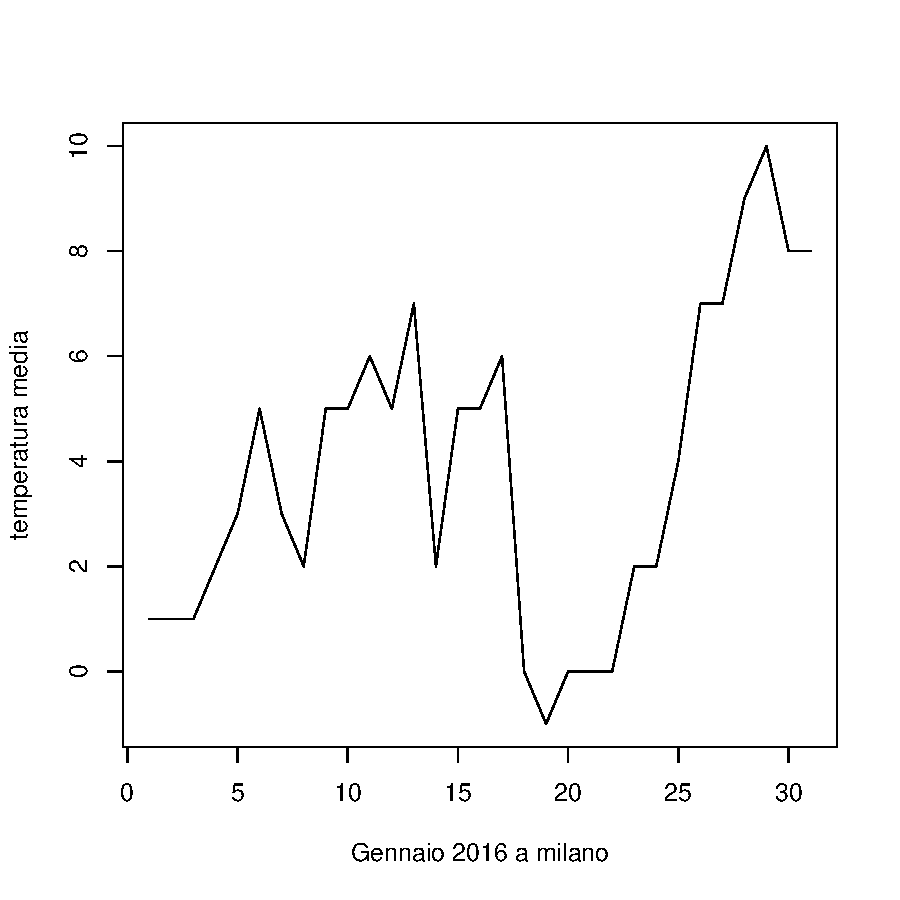
\includegraphics{RbookParte2-111}
\caption{ Andamento della temperatura a Gennaio 2016  a Milano. }
\label{fig:datiist}
\end{center}
\end{figure}

Raggruppiamo ora i dati in classi comprese  tra due estremi che comprendano certamente tutti i dati, per esempio -2 e 10, decidendo di applicare un passo di 2 e vedere come si distribuiscono. Il comando \texttt{cut} associa a ciascun dato la classe di appartenenza selezionata in base ai punti di taglio.

\begin{Schunk}
\begin{Sinput}
> tagli=c(-2,0,2,4,6,10)
> cut(Milano,breaks=tagli)
\end{Sinput}
\begin{Soutput}
 [1] (0,2]  (0,2]  (0,2]  (0,2]  (2,4]  (4,6]  (2,4]  (0,2] 
 [9] (4,6]  (4,6]  (4,6]  (4,6]  (6,10] (0,2]  (4,6]  (4,6] 
[17] (4,6]  (-2,0] (-2,0] (-2,0] (-2,0] (-2,0] (0,2]  (0,2] 
[25] (2,4]  (6,10] (6,10] (6,10] (6,10] (6,10] (6,10]
Levels: (-2,0] (0,2] (2,4] (4,6] (6,10]
\end{Soutput}
\end{Schunk}

Il comando \texttt{table} conta i dati di ciascuna classe

\begin{Schunk}
\begin{Sinput}
> table(cut(Milano,breaks=tagli))
\end{Sinput}
\begin{Soutput}
(-2,0]  (0,2]  (2,4]  (4,6] (6,10] 
     5      8      3      8      7 
\end{Soutput}
\end{Schunk}
Si noti che la suddivisione in classi prevede intervalli aperti a sinistra e chiusi a destra.
Per suddividere in modo che gli intervalli siano chiusi a sinistra e aperti a destra si specifica il parametro \texttt{right=FALSE}.
Possiamo anche usare il comando \texttt{seq} per specificare i tagli.
 \begin{eqnarray*}
\texttt{table(cut}( \varia{variabile},\texttt{breaks=seq}(\varia{estremo inf},\\
\varia{estremo sup},\texttt{by}=\varia{passo}),\texttt{right=TRUE}))
\end{eqnarray*}
o in modo  pi\`u generale
\begin{eqnarray*}
&\texttt{table(cut}(\varia{ variabile},\\
&\texttt{breaks=c}(\varia{estremo\; inferiore}, \ldots,\varia{estremo superiore}))
\end{eqnarray*}
estremamente utile in quanto consente di raggruppare i dati in classi non necessariamente di ugual ampiezza.
\begin{Schunk}
\begin{Sinput}
> table(cut(Milano,breaks=c(-3,1,3,4,5,6,8,10)))
\end{Sinput}
\begin{Soutput}
(-3,1]  (1,3]  (3,4]  (4,5]  (5,6]  (6,8] (8,10] 
     8      7      1      6      2      5      2 
\end{Soutput}
\end{Schunk}
Volendo raggruppare in classi i dati delle precedenti uscite del dado possiamo scrivere
\begin{Schunk}
\begin{Sinput}
> table(cut(dadi100,breaks=0:6))
\end{Sinput}
\begin{Soutput}
(0,1] (1,2] (2,3] (3,4] (4,5] (5,6] 
   15    25    11    17    18    14 
\end{Soutput}
\end{Schunk}
Se scegliamo di chiudere a sinistra gli intervalli dobbiamo però includere il 7 altrimenti 
il valore 6 non risutlerebbe incluso.
\begin{Schunk}
\begin{Sinput}
> table(cut(dadi100,breaks= 1:7,right=FALSE))
\end{Sinput}
\begin{Soutput}
[1,2) [2,3) [3,4) [4,5) [5,6) [6,7) 
   15    25    11    17    18    14 
\end{Soutput}
\end{Schunk}

\subsection{Areogrammi}
Il comando generico per generare un istogramma \`e:
\begin{equation*}
\texttt{hist}(\varia{variabile})
\end{equation*}
che segue per\`o la struttura del comando \texttt{cut}. L'ampiezza di ciascuna classe salvo diversamente indicato \`e costante e decisa da \textsf{R}.
\`E  possibile variare tale condizione definendo una lista con i punti di taglio ({\it cutoff}) delle classi volute:
\begin{equation} \texttt{hist}(\varia{variabile},\texttt{c}(\varia{valore}_1, \varia{valore}_2, \ldots))
\end{equation}
Per esempio se \texttt{dadi100} rappresenta le solite 100 uscite del lancio del dado, il comando
\begin{Schunk}
\begin{Sinput}
> par(mfrow=c(1,2))
> hist(dadi100,breaks=seq(0.5,6.5,1),col="red")
> hist(dadi100,freq=FALSE,breaks=seq(0.5,6.5,1),col="blue")
\end{Sinput}
\end{Schunk}
\begin{figure}[htbp]
\begin{center}
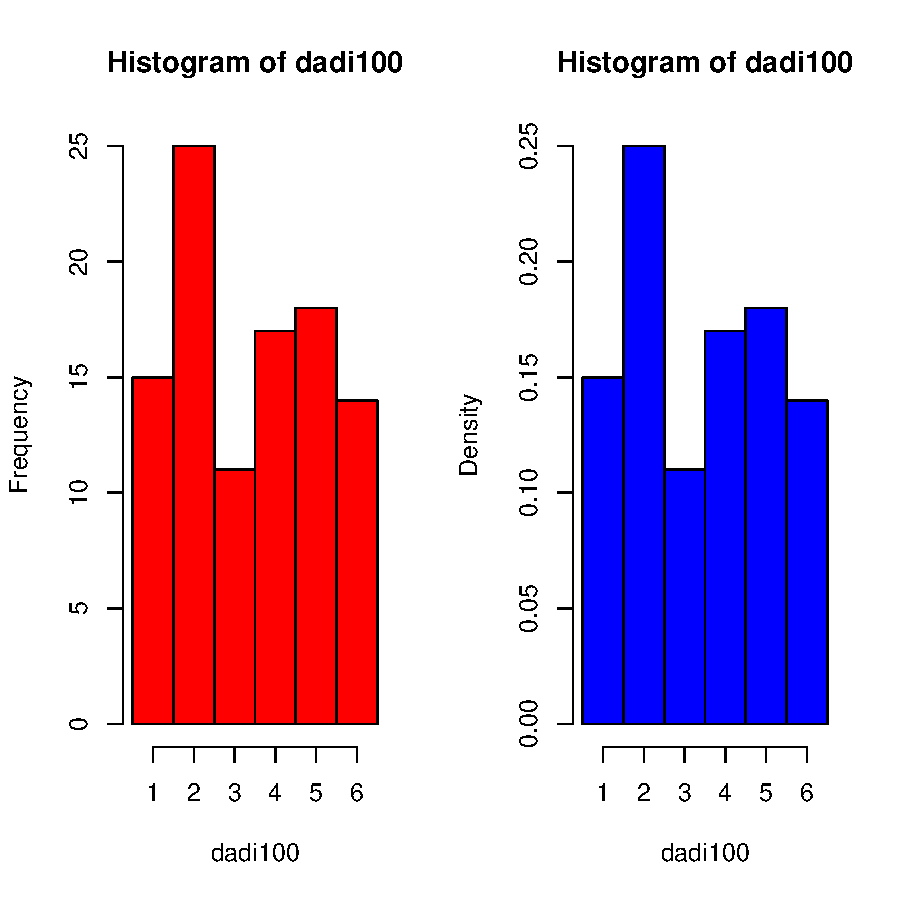
\includegraphics{RbookParte2-118}
\caption{Diagramma a colonne e areogramma per il lancio di un dado.}
\label{fig:datidado}
\end{center}
\end{figure}
genera l'istogramma (in rosso, a sinistra Figura~\ref{fig:datiist}) con le frequenze assolute delle classi in ordinata. La sequenza dei punti di taglio \`e stata scelta in modo che i numeri interi da 1 a 6 siano al centro delle classi corrispondenti. Se invece volessimo creare un areogramma  (ossia avere un tracciato per cui le aree siano pari alle frequenze relative) a partire dalle stesse uscite dovremo imporre il parametro \texttt{freq=FALSE} otterremo il pannello a destra (in blu) della figura~(\ref{fig:datiist}). Avendo scelto classi di ampiezza costante i 2 grafici differiscono semplicemente per un cambio di scala sull'asse $y$.

In modo simile possiamo tracciare un areogramma  dei dati nella variabile \texttt{milano}
\begin{Schunk}
\begin{Sinput}
> par(mfrow=c(1,2))
> hist(Milano, col="green",freq=FALSE,right=FALSE,
+ main="Cutoff automatici")
\end{Sinput}
\end{Schunk}
lasciando \textsf{R} libero di scegliere i punti di taglio (pannelli a sinistra della figura \ref{fig:datiistmilano}) o scegliendoli a nostra volta (pannelli a destra della stessa figura  \ref{fig:datiistmilano})
\begin{Schunk}
\begin{Sinput}
> hist(Milano,col="red",freq=FALSE,
+ breaks=unique(as.vector(quantile(Milano,seq(0,1,by=1/6)))),
+ main="Cutoff personalizzati")
\end{Sinput}
\end{Schunk}
\begin{figure}[htbp]
\begin{center}
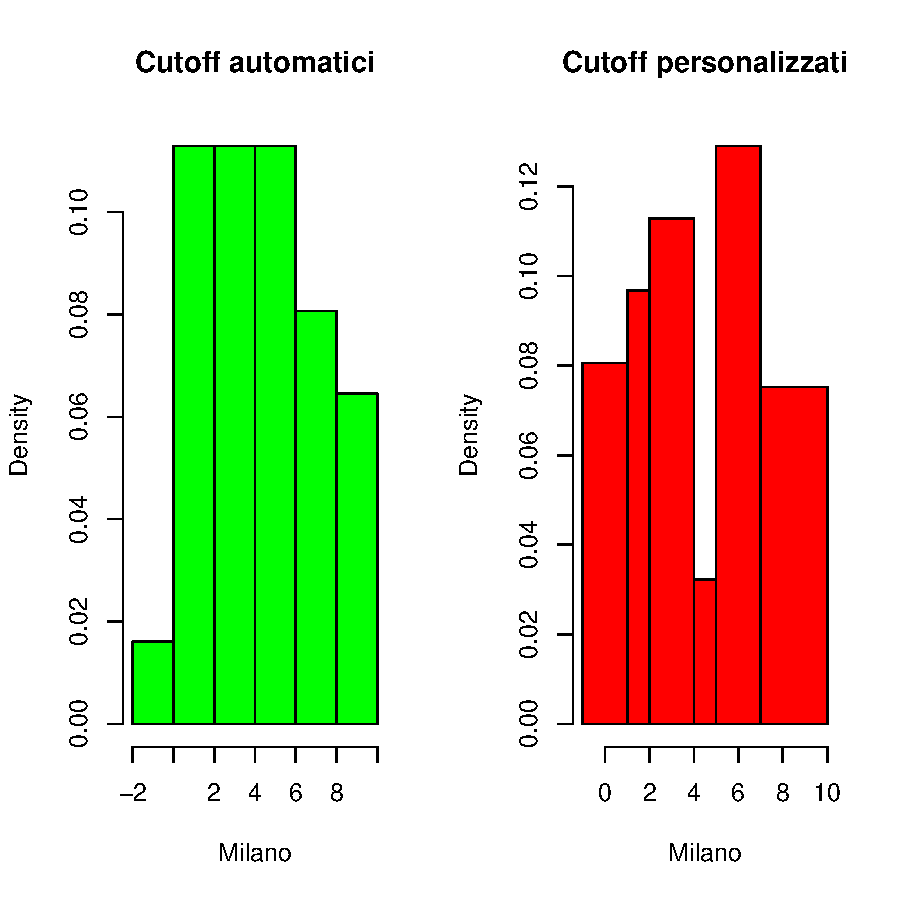
\includegraphics{RbookParte2-122}
\caption{ Areogramma dei dati della temperatura. Scelta automatica dei punti di taglio.}
\label{fig:datiistmilano}
\end{center}
\end{figure}
Si noti la stabilit\`a degli areogrammi rispetto ai cambi nella suddivisione.
\subsection{Generazione di boxplot}

Il \texttt{boxplot}  \`e una rappresentazione grafica immediata della statistica dei 5 numeri e simultaneamente ci  segnala eventuali punti discordanti o anomali, {\it outlier}.
Il comando generico \`e: \begin{equation}\texttt{boxplot}(\varia{variabile})\end{equation}
prendendo il vettore $x$ contenente i risultati di 100 lanci
otteniamo la figura~\ref{fig:boxplotdado}
\begin{figure}[htbp]
\begin{center}
\begin{Schunk}
\begin{Sinput}
> boxplot(dadi100)
\end{Sinput}
\end{Schunk}
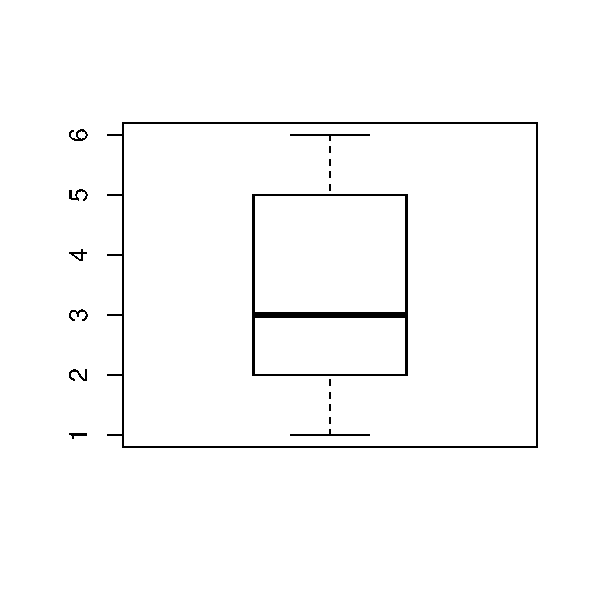
\includegraphics{RbookParte2-123}
\caption{Boxplot dei risultati del lancio di un dado}
\label{fig:boxplotdado}
\end{center}
\end{figure}
da cui si evince che il valore massimo dei dati \`e 6, il minimo \`e 1 e non ci sono punti anomali, per cui non vi sono dati anomali, altrimenti evidenziati da un pallino. Si legge inoltre il valore di mediana (4) primo quartile (2) e terzo quartile (5).

\subsection{Creazione di grafici a torta}

Il comando \texttt{pie} consente, partendo da una tabella, di tracciare il diagramma a torta per una variabile nominale raggruppata in classi. Il comando \`e

\begin{equation*}\texttt{pie(table}(\varia{variabile} ))
\end{equation*}
ad esempio (facendo riferimento ai precedenti dati):
\begin{Schunk}
\begin{Sinput}
> pie(table(dadi100))
\end{Sinput}
\end{Schunk}
fornisce in uscita  la Figura~\ref{fig:pie}
\begin{figure}[htbp]
\begin{center}
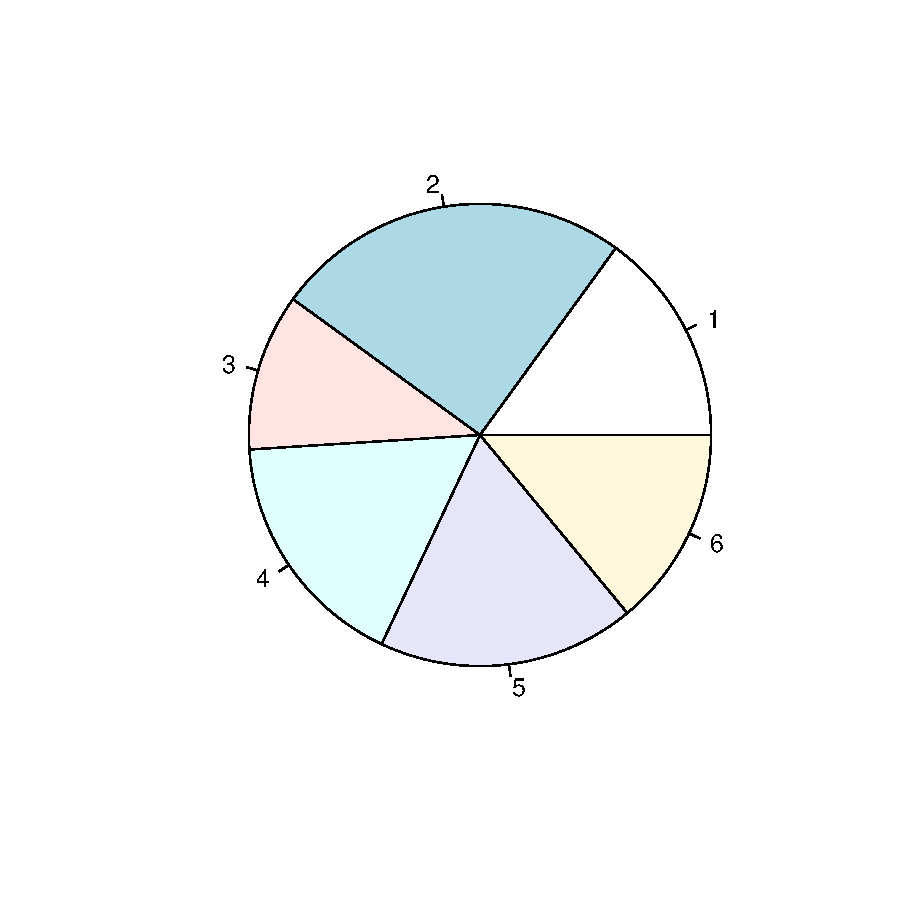
\includegraphics{RbookParte2-125}
\caption{Diagramma a torta per il lancio di un dado equo.}
\label{fig:pie}
\end{center}
\end{figure}
\begin{shaded}{Costruire una matrice contenente le coordinate di 50 punti nel rettangolo $[0,4]\times [0,2]$ in due dimensioni (generate utilizzando il generatore di numeri pseudocasuali). Produrre un grafico con due pannelli, dove il primo pannello \`e uno scatter-plot}
\end{shaded}
\section{Variabili doppie e rette di regressione}
Supponiamo di misurare la concentrazione di acido lattico muscolare durante uno sforzo di 10 minuti,
\begin{Schunk}
\begin{Sinput}
> x<-tempo<-c(1,2,3,4,5,6,7,8,9,10)
> y<-concentrazione<-c(0.3,0.65,0.7,0.8,0.95,1.05,1.3,1.7,1.9,
+ 2.5)
\end{Sinput}
\end{Schunk}
Per analizzare questi dati conviene preliminarmente tracciarne un diagramma a dispersione.
\begin{figure}[htbp]
\begin{center}
\begin{Schunk}
\begin{Sinput}
> plot(x,y)
\end{Sinput}
\end{Schunk}
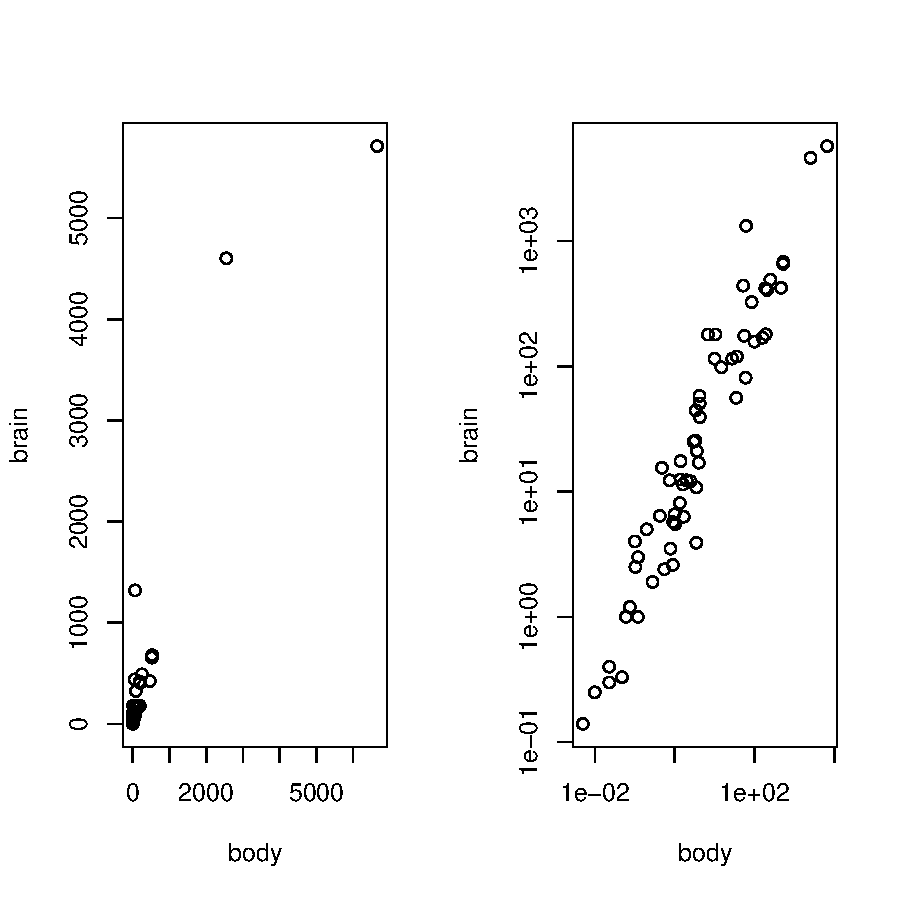
\includegraphics{RbookParte2-127}
\caption{Diagramma a dispersione tempo/concentrazione.}
\label{fig:scatte}
\end{center}
\end{figure}
Possiamo inoltre determinare il coefficiente di correlazione lineare
\begin{Schunk}
\begin{Sinput}
> cor(x,y)
\end{Sinput}
\begin{Soutput}
[1] 0.9620456
\end{Soutput}
\end{Schunk}
Per definire un modello di relazione lineare occorre usare il comando \texttt{lm} (\varia{linear model}).
Nella sua generica forma il comando \`e espresso come\footnote{ Per digitare la tilde  \mytilde\;  su Mac premere ALT 5 su PC invece il tasto Alt Gr (attivazione del codice ASCII) e sul tastierino numerico digitare il numero 126. Lavorando su un portatile il tastierino numerico \`e spesso incorporato nella tastiera con colorazione blu dei tasti.}
$$\texttt{lm}(\varia{y} \sim  \varia{x})$$
Otteniamo i valori di pendenza e intercetta.

Possiamo tracciare la retta di regressione con il comando \texttt{abline}.
\begin{Schunk}
\begin{Sinput}
> plot(x,y,pch=19,col="red")
> abline(lm(y~x),col="blue")
\end{Sinput}
\end{Schunk}
Per determinare  la retta di regressione sulle $y$ dobbiamo invertire $x$ e $y$.
\begin{Schunk}
\begin{Sinput}
> (modellox=lm(x~y))
\end{Sinput}
\begin{Soutput}
Call:
lm(formula = x ~ y)

Coefficients:
(Intercept)            y  
     0.3516       4.3446  
\end{Soutput}
\begin{Sinput}
> coeff=modellox$coefficients
> (a=1/coeff[2])
\end{Sinput}
\begin{Soutput}
        y 
0.2301707 
\end{Soutput}
\begin{Sinput}
> (b=-coeff[1]/coeff[2])
\end{Sinput}
\begin{Soutput}
(Intercept) 
-0.08093883 
\end{Soutput}
\begin{Sinput}
> abline(b,a,col="green")
\end{Sinput}
\end{Schunk}
In tal modo otteniamo il grafico~\ref{fig:duerettex}.
\begin{center}
\begin{figure}[htbp]
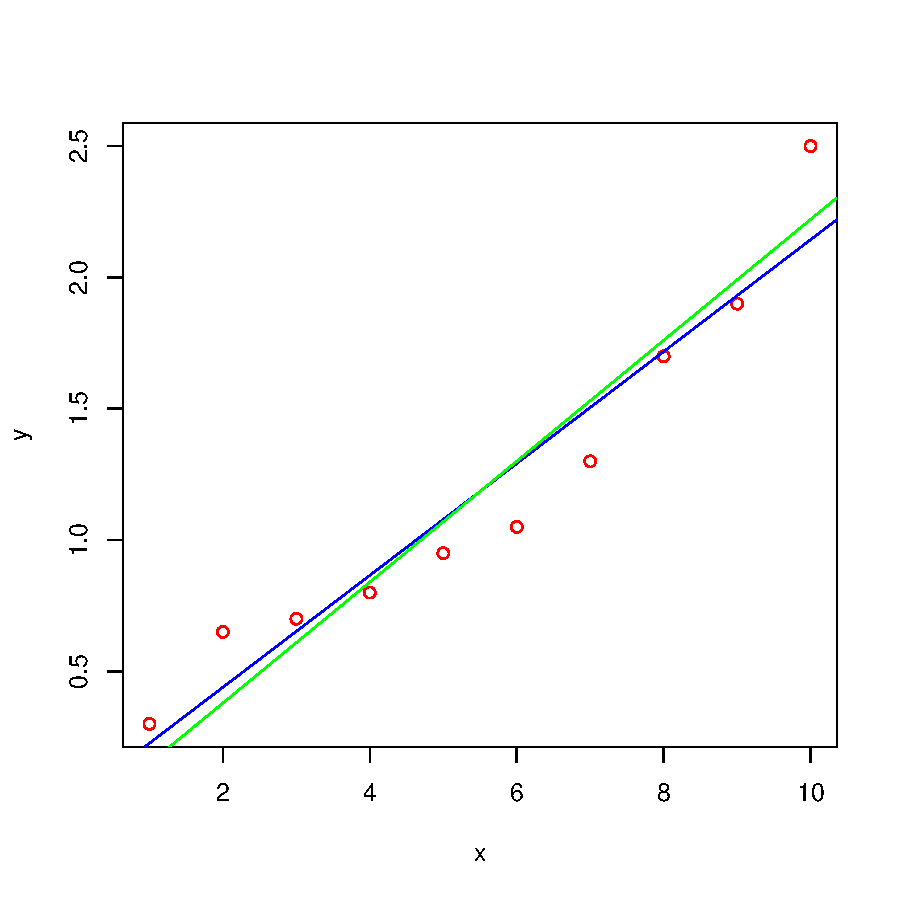
\includegraphics{RbookParte2-131}
\caption{Rette di regressione. In blu $R_x$, in verde $R_y$.}
\label{fig:duerettex}
\end{figure}
\end{center}

\subsubsection{I bambini di Kalama (Egitto). Ancora retta di regressione}
Da DASL \cite{DASL} possiamo scaricare un \emph{dataset} in cui i ricercatori hanno misurato le altezze (cm) dai 18 ai 29 mesi di vita, di 161 bambini di Kalama, un villaggio egiziano. Le altezze sono state mediate tra i bambini per fornire un singolo valore mese per mese.
\begin{Schunk}
\begin{Sinput}
> age=18:29
> height=c(76.1,77,78.1,78.2,78.8,79.7,79.9,81.1,81.2,81.8,82.8,83.5)
\end{Sinput}
\end{Schunk}
Possiamo quindi costruire il \texttt{data.frame}
\begin{Schunk}
\begin{Sinput}
> village=data.frame(age=age,height=height)
\end{Sinput}
\end{Schunk}
Ora diamo una prima occhiata ai dati:
 %code chunk
\begin{figure}[htbp]
\begin{center}
\begin{Schunk}
\begin{Sinput}
> plot(age,height)
\end{Sinput}
\end{Schunk}
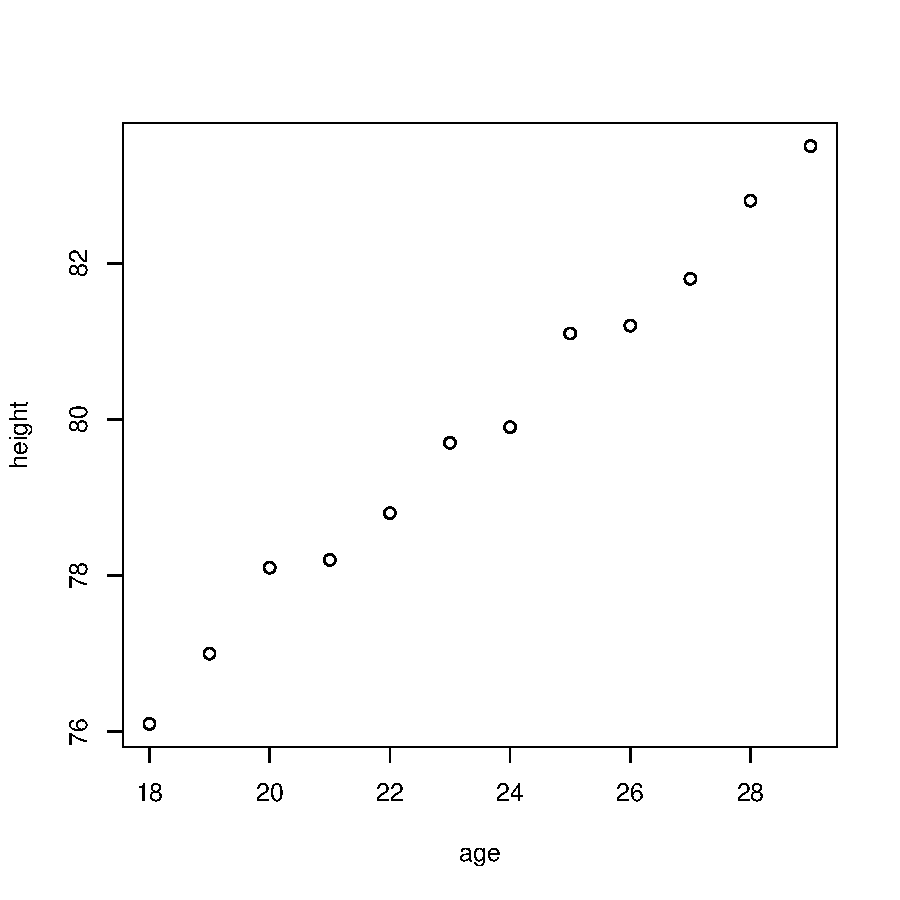
\includegraphics{RbookParte2-134}
\caption{Crescita dei bambini di Kalama}
\label{kalama}
\end{center}
\end{figure}
L'andamento \`e lineare. Determiniamo la retta di regressione
per predire l'altezza media nota l'et\`a in mesi.
%code chunk
\begin{Schunk}
\begin{Sinput}
> (modello=lm(height~age))
\end{Sinput}
\begin{Soutput}
Call:
lm(formula = height ~ age)

Coefficients:
(Intercept)          age  
     64.928        0.635  
\end{Soutput}
\end{Schunk}
La retta di regressione cercata ha formula:
$$h(\texttt{age})=64.93+ 0.63\, \texttt{age}$$

Possiamo ora utilizzare \textsf{R} come semplice calcolatore per predire l'altezza a 27.5 mesi di et\`a:
oppure, \`e pi\`u  efficiente utilizzare direttamente il \emph{dataframe} e la funzione
\texttt{predict}:
%codechunk
\begin{Schunk}
\begin{Sinput}
> predict(modello,data.frame(age=27.5))
\end{Sinput}
\begin{Soutput}
       1 
82.38986 
\end{Soutput}
\end{Schunk}
fornendo in input i parametri della retta ed un preciso valore della variabile indipendente (richiamata col proprio nome).
Molti comandi di \textsf{R} sono in grado di manipolare \emph{dataframe}  lavorando direttamente sulla struttura. Per esempio, il comando plot di un \texttt{dataframe} in due colonne, esegue in automatico il grafico della seconda colonna (variabile dipendente) vs prima colonna (variabile indipendente).
Possiamo ottenere il modello lineare visto nel caso precedente, passando \texttt{village} direttamente al comando:
\begin{Schunk}
\begin{Sinput}
> modello=lm(height~age,data=village)
> modello
\end{Sinput}
\begin{Soutput}
Call:
lm(formula = height ~ age, data = village)

Coefficients:
(Intercept)          age  
     64.928        0.635  
\end{Soutput}
\end{Schunk}
con la formula $lm(y \tilde{} x,data=dataset)$.
Inoltre possiammo considerare il plot di un oggetto \texttt{lm}  che fornisce una serie di rappresentazioni grafiche
\begin{Schunk}
\begin{Soutput}
$mfrow
[1] 1 1
\end{Soutput}
\end{Schunk}
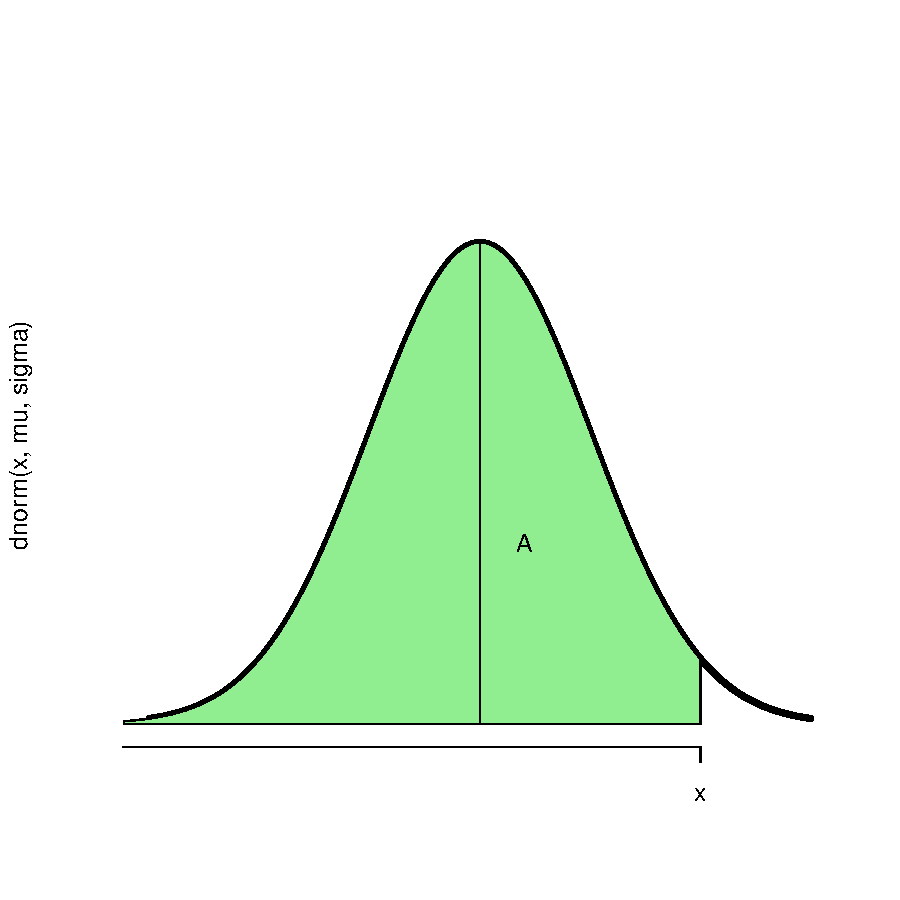
\includegraphics{RbookParte2-138}
\section{Modelli potenza}
Consideriamo ora il seguente \emph{dataset} di mammiferi  in cui le 2 variabili rappresentano  le dimensioni del corpo e del cervello.
\begin{Schunk}
\begin{Sinput}
> library(MASS)
> mammals
\end{Sinput}
\begin{Soutput}
                              body   brain
Arctic fox                   3.385   44.50
Owl monkey                   0.480   15.50
Mountain beaver              1.350    8.10
Cow                        465.000  423.00
Grey wolf                   36.330  119.50
Goat                        27.660  115.00
Roe deer                    14.830   98.20
Guinea pig                   1.040    5.50
Verbet                       4.190   58.00
Chinchilla                   0.425    6.40
Ground squirrel              0.101    4.00
Arctic ground squirrel       0.920    5.70
African giant pouched rat    1.000    6.60
Lesser short-tailed shrew    0.005    0.14
Star-nosed mole              0.060    1.00
Nine-banded armadillo        3.500   10.80
Tree hyrax                   2.000   12.30
N.A. opossum                 1.700    6.30
Asian elephant            2547.000 4603.00
Big brown bat                0.023    0.30
Donkey                     187.100  419.00
Horse                      521.000  655.00
European hedgehog            0.785    3.50
Patas monkey                10.000  115.00
Cat                          3.300   25.60
Galago                       0.200    5.00
Genet                        1.410   17.50
Giraffe                    529.000  680.00
Gorilla                    207.000  406.00
Grey seal                   85.000  325.00
Rock hyrax-a                 0.750   12.30
Human                       62.000 1320.00
African elephant          6654.000 5712.00
Water opossum                3.500    3.90
Rhesus monkey                6.800  179.00
Kangaroo                    35.000   56.00
Yellow-bellied marmot        4.050   17.00
Golden hamster               0.120    1.00
Mouse                        0.023    0.40
Little brown bat             0.010    0.25
Slow loris                   1.400   12.50
Okapi                      250.000  490.00
Rabbit                       2.500   12.10
Sheep                       55.500  175.00
Jaguar                     100.000  157.00
Chimpanzee                  52.160  440.00
Baboon                      10.550  179.50
Desert hedgehog              0.550    2.40
Giant armadillo             60.000   81.00
Rock hyrax-b                 3.600   21.00
Raccoon                      4.288   39.20
Rat                          0.280    1.90
E. American mole             0.075    1.20
Mole rat                     0.122    3.00
Musk shrew                   0.048    0.33
Pig                        192.000  180.00
Echidna                      3.000   25.00
Brazilian tapir            160.000  169.00
Tenrec                       0.900    2.60
Phalanger                    1.620   11.40
Tree shrew                   0.104    2.50
Red fox                      4.235   50.40
\end{Soutput}
\end{Schunk}
Per prima cosa tracciamo il grafico dei punti  in scala non trasformata e, visto la compresenza di dati molto prossimi all'origine e di dati molto distanti in scala logaritmica (sia le $x$ che le $y$ vengono trasformate prendendone i logaritmi)
\begin{Schunk}
\begin{Sinput}
> par(mfrow=c(1,2))
> plot(mammals)
> plot(mammals,log="xy")
\end{Sinput}
\end{Schunk}
come in Figura~\ref{fig:duemammals}.\begin{figure}[htbp]
\begin{center}
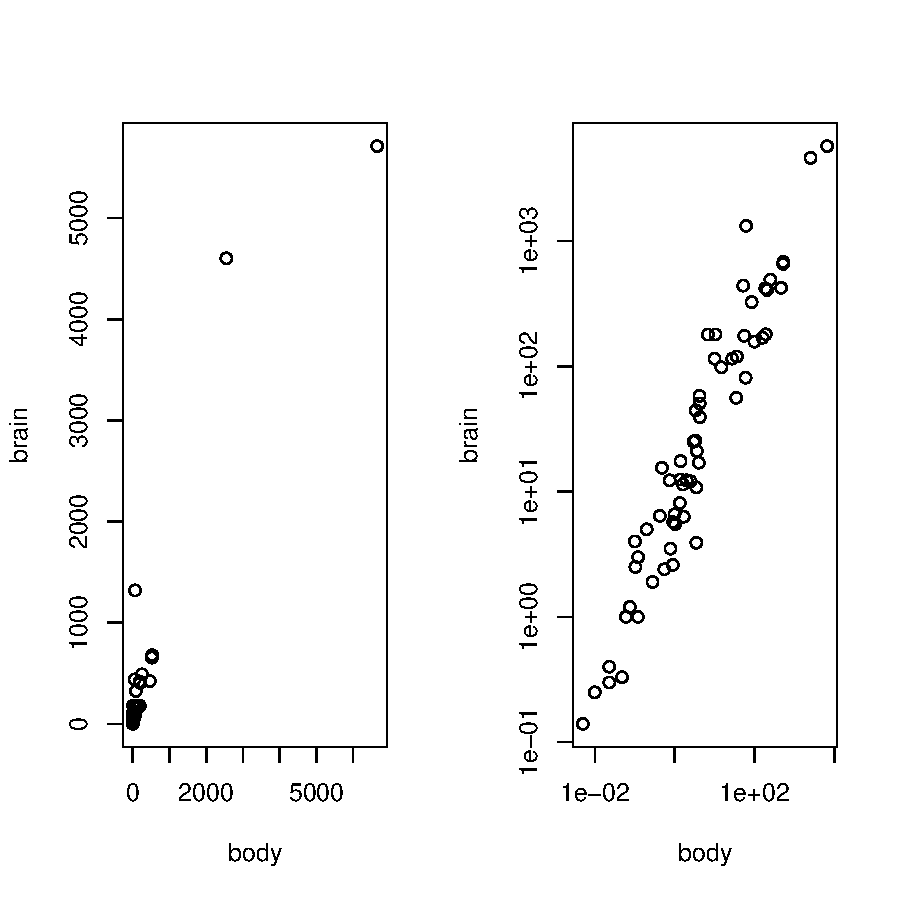
\includegraphics{RbookParte2-141}
\caption{Diagramma a dispersione massa corporea/massa del cervello in scala normale ed in scala logaritmica. }
\label{fig:duemammals}
\end{center}
\end{figure}
Visti i  risultati ottenuti usando la scala logaritmica tracciamo anche la corrispondente retta di regressione
\begin{Schunk}
\begin{Sinput}
> plot(log(mammals$brain)~log(mammals$body),col="BLUE",pch=19,type="p")
> abline(lm(log(mammals$brain)~ log(mammals$body)),col="red",lwd=3);
> uomo=which(rownames(mammals)=="Human")
> text(log(mammals[uomo ,1]),log(mammals[uomo ,2]),rownames(mammals)[uomo])
\end{Sinput}
\end{Schunk}
\begin{figure}[htbp]
\begin{center}
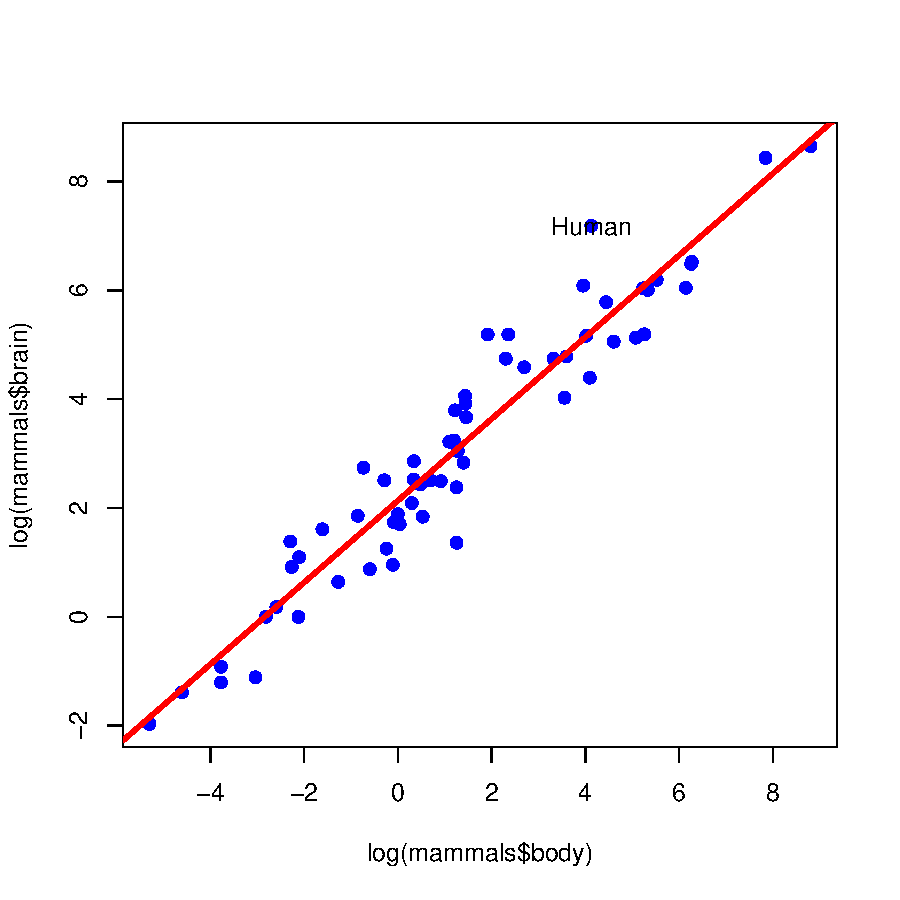
\includegraphics{RbookParte2-143}
\caption{ Retta di regressione. Dimensione del corpo e del cervello. Si noti la posizione dell'uomo.}
\label{duerette}
\end{center}
\end{figure}
Si noti il comando \texttt{text(\varia{x},\varia{y}, \varia{testo})}
dove    $\varia{x}$ e $\varia{y}$  e $\varia{testo}$ sono vettori di arbitraria lunghezza contenenti ascisse, ordinate e testo da inserire.
\section{Distribuzioni in \textsf{R}}
I nomi delle principali distribuzioni in \textsf{R} sono\vskip10pt
\begin{tabular}{|r|c |}
\hline
\texttt{norm}&normale\\
\texttt{t}  &Student\\
\texttt{chisq}& chi quadro\\
\texttt{f}&Fisher\\
\texttt{binom }&binomiale\\
\hline
\end{tabular}\vskip10pt
A questi nomi possiamo aggiungere diversi prefissi\vskip10pt
\begin{tabular}{|r|c |}
\hline
\texttt{d}&densit\`a\\
\texttt{p}  &primitiva\\
\texttt{q}& quantile\\
\texttt{r}&random\\
  \hline
\end{tabular}
\vskip10pt
per caratterizzare diversi aspetti.
\begin{comment}
\begin{itemize}
\begin{question}
  Figure~\ref{fig:scatterplot} shows a scatterplot. Which of the
  following statements are correct?


\begin{figure}[htb!]
\begin{center}
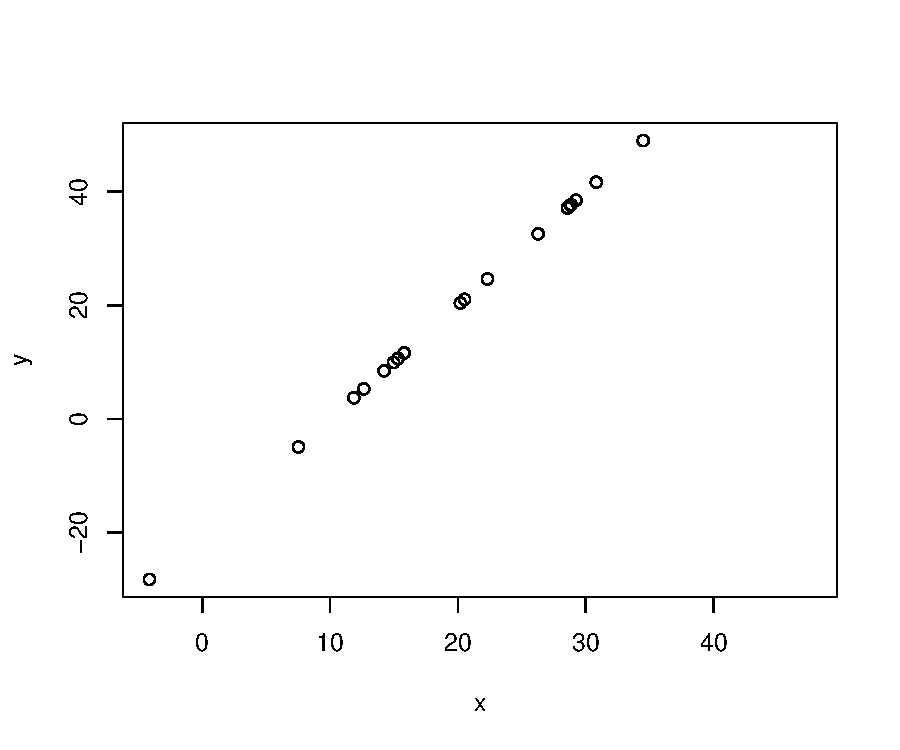
\includegraphics{RbookParte2-145}
\caption{ Scatterplot}\label{fig:scatterplot}
\end{center}
\end{figure}

\begin{answerlist}
  \item The standard deviation of $Y$ is at least $6$.
  \item For $X =  13.6 $, $Y$ can be expected to be about  -44 .
  \item La pendenza della retta di regressione ? circa $1$.
  \item The mean of $X$ is at most $5$.
  \item The absolute value of the correlation coefficient is at most $0.8$.
\end{answerlist}
\end{question}

%% SOLUTIONS
\begin{solution}
\begin{answerlist}
  \item \textbf{True}: The standard deviation of $Y$ is about equal to $ 20 $ and is therefore larger than $6$.
  \item \textbf{False}: The regression line at $X=13.6$ implies a value of about $Y = 7.2$.
  \item \textbf{False}: The slope of the regression line is given by $r \cdot s_y/s_x$ and hence not about equal to $1$.
  \item \textbf{False}: The mean of $X$ is about equal to $ 20 $ and hence is larger than $5$.
  \item \textbf{False}: A strong association between the variables is given in the scatterplot. Hence the absolute value of the correlation coefficient is close to $1$ and therefore larger than $0.8$.
\end{answerlist}
\end{solution}
\end{itemize}
%% META-INFORMATION
%% \extype{mchoice}
%% \exsolution{10000}
%% \exname{Multiple choice}

\end{comment}
\subsection{Distribuzione normale}
\subsubsection{La funzione \texttt{dnorm}}
Come appena visto \textsf{R }indica con il nome \texttt{dnorm}, la densit\`a normale o gaussiana. Essa accetta come parametri sia la media $\mu$ che la deviazione standard $\sigma$ come \`e possibile verificare con il comando \texttt{formals} che ci fornisce gli argomenti di una funzione e gli eventuali valori preassegnati.
\begin{Schunk}
\begin{Sinput}
> formals(dnorm)
\end{Sinput}
\begin{Soutput}
$x


$mean
[1] 0

$sd
[1] 1

$log
[1] FALSE
\end{Soutput}
\end{Schunk}
Se i parametri sono omessi \texttt{dnorm} rappresenta la densit\`a normale standard con $\mu=0$ e $\sigma=1$.
Il grafico~(\ref{fig:normalesta}) della gaussiana
 tra due estremi, ad esempio -2.5 e 2.5 si ottiene con il solito comando
\begin{Schunk}
\begin{Sinput}
> curve(dnorm,-2.5,2.5)
\end{Sinput}
\end{Schunk}

\begin{figure}[htbp]
\begin{center}
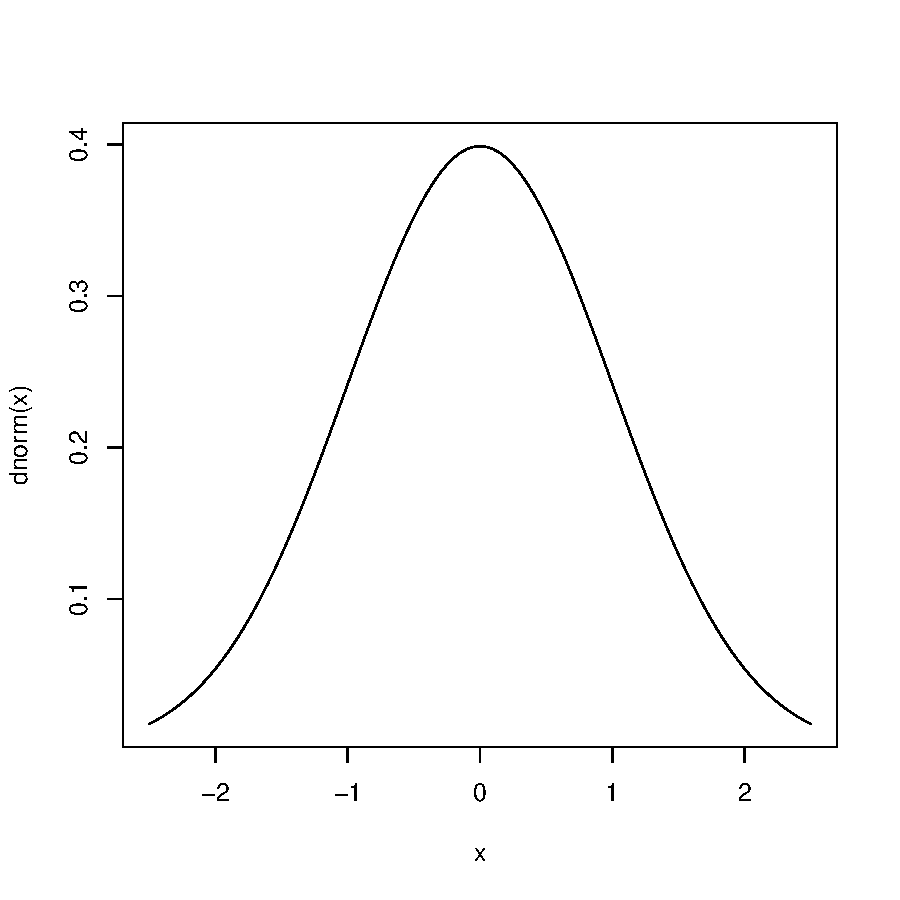
\includegraphics{RbookParte2-148}
\caption{ Grafico della normale standard nell'intervallo $[-2.5,2.5]$. }
\label{fig:normalesta}
\end{center}
\end{figure}
Per  visualizzare una gaussiana non standard, ad esempio una gaussiana con media $\mu=1$ e  deviazione standard $\sigma=1.5$, tra -3 e 3. scriveremo invece
\begin{Schunk}
\begin{Sinput}
> curve(dnorm(x,mean=1,sd=1.5),-3,3)
\end{Sinput}
\end{Schunk}
\subsection{La funzione \texttt{pnorm}}
La funzione \texttt{pnorm}(\varia{x})   \`e la antiderivata di \texttt{dnorm} calcolata come segue
\begin{equation*}\texttt{pnorm}(\varia{x}) =\int_{-\infty}^x  \texttt{dnorm}(s)ds
\end{equation*}
Ovviamente
$$\int_a^b \texttt{dnorm}(x)dx=\texttt{pnorm}(b)-\texttt{pnorm}(a)$$
e per avere l'area sottesa tra $3$ e $5$  basta scrivere:
\begin{Schunk}
\begin{Sinput}
> pnorm(5)-pnorm(3)
\end{Sinput}
\begin{Soutput}
[1] 0.001349611
\end{Soutput}
\end{Schunk}

Per ottenere il valore dell'area tra 0 e $x$ bisogna allora sottrarre \texttt{pnorm}(0)=0.5 all'area fornita dalla funzione.
Per cui possiamo scrivere:
\begin{Schunk}
\begin{Sinput}
> pnorm(1)-0.5
\end{Sinput}
\begin{Soutput}
[1] 0.3413447
\end{Soutput}
\end{Schunk}


\subsection{La funzione \texttt{qnorm} e la tabella della densit\`a di Gauss}

La funzione \texttt{qnorm} rappresenta la funzione inversa di \texttt{pnorm}.
\[\texttt{qnorm}(A)=x\Leftrightarrow A=\int_{-\infty}^x \texttt{dnorm}(s)ds\] 
come illustrato nella figura~\ref{fig:fig2code}.
\begin{center}
\begin{figure}[H]
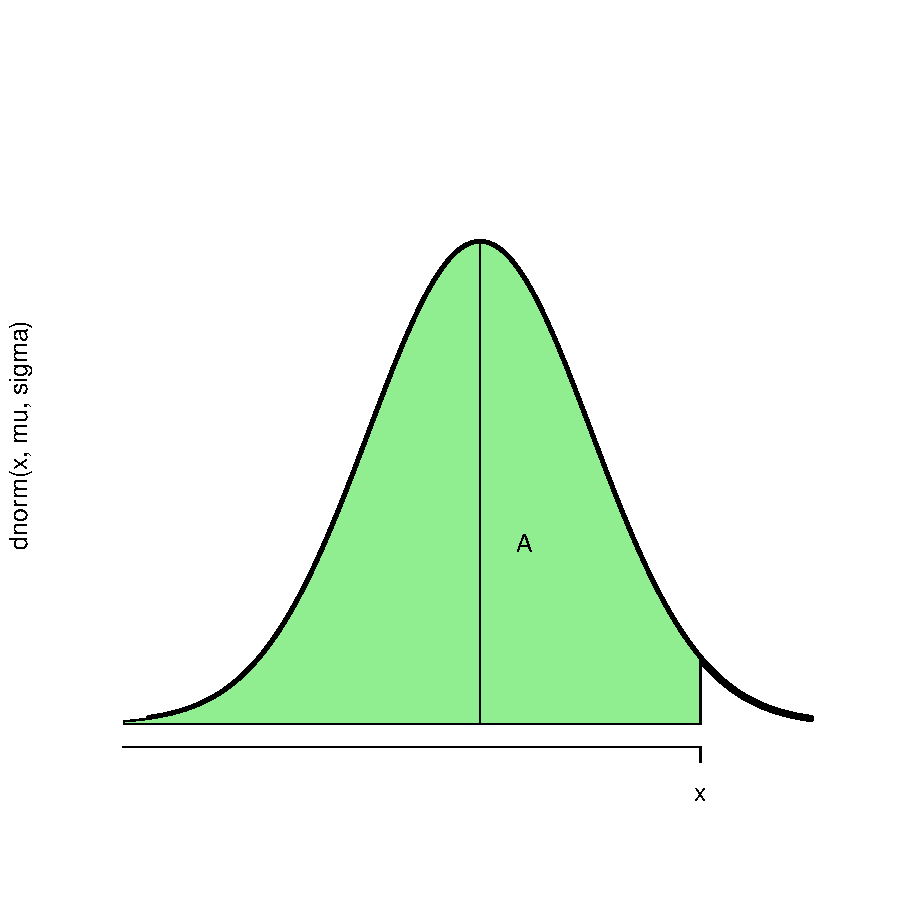
\includegraphics{RbookParte2-153}
\caption{$x=\texttt{qnorm}(A)$}
\label{fig:fig2code}
\end{figure}
\end{center}
Vogliamo costruire una funzione, diciamo $U$ tale che assegnato un valore di area $A$   fornisca l'ascissa $x=U(A)$ come in figura~\ref{fig:fig12code} in modo che l'area tra - $x$ e $x$ sia esattamente pari ad $A$.  

\begin{figure}[H]
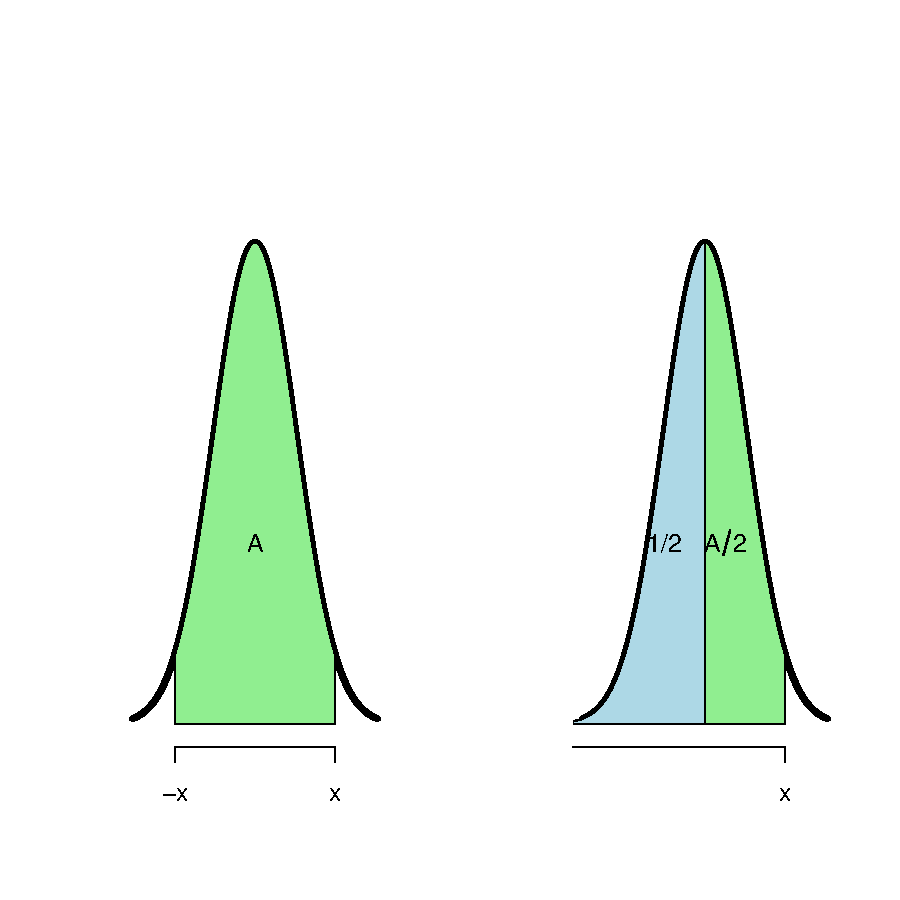
\includegraphics{RbookParte2-154}
\caption{$x=U(A)=\texttt{qnorm}(1/2+A/2)$}
\label{fig:fig12code}
\end{figure}
Dalla stessa figura  si evince che la funzione che riproduce la tabella è
\begin{Schunk}
\begin{Sinput}
> U <-function (A) qnorm (1/2 + A/2)
\end{Sinput}
\end{Schunk}
Questa funzione fornisce fissato il livello di fiducia l'ascissa $x$  tale che l'intervallo simmetrico $[-x,x]$ racchiuda un'area pari al lvello di fiducia. Per esempio
\begin{Schunk}
\begin{Sinput}
> U(0.95)
\end{Sinput}
\begin{Soutput}
[1] 1.959964
\end{Soutput}
\end{Schunk}
\begin{figure}[htbp]
\begin{center}
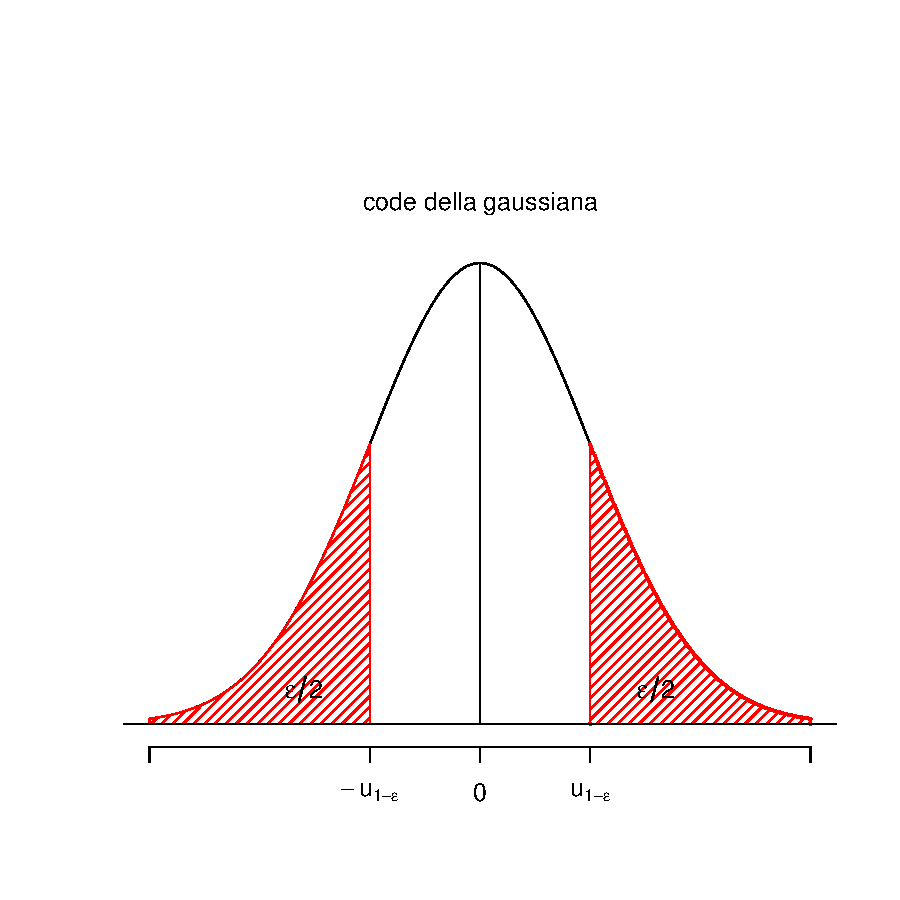
\includegraphics{RbookParte2-158}
\caption{Code della distribuzione normale}
\label{fig:normaletratto}
\end{center}
\end{figure}

 \subsection{La funzione \texttt{rnorm}}
\`E possibile generare dei valori standardizzati casuali (media uguale a 0, deviazione standard pari a 1) che seguono la distribuzione normale standard. Basta semplicemente definire il numero di valori desiderati.
Il comando nella sua espressione generale \`e:
\begin{equation}\texttt{rnorm}(n,\texttt{mean}=\varia{valore}_1,\texttt{sd}=\varia{valore}_2)\end{equation}
Nel caso in cui volessimo una lista di 20 valori di una variabile normale con media assegnata 5 e deviazione standard 1 scriveremo :

\begin{Schunk}
\begin{Sinput}
> rnorm(20,mean=5,sd=1)
\end{Sinput}
\end{Schunk}
\subsection{La distribuzione $t$ di Student}
In \textsf{R} la distribuzione di Student \`e indicata con la lettera  \texttt{t}.  Come per le altre densit\`a  si possono considerare le funzioni\vskip5pt
\begin{tabular}{|r|r |}
\hline
dt  &densit\`a\\
pt  &primitiva\\
qt & quantili\\
rt  &generatore random\\
\hline
\end{tabular}
\vskip10pt
Il grafico della distribuzione di Student ad un certo numero \texttt{df} di gradi di libert\`a  si ottiene con il comando
\begin{equation*}
\texttt{curve(dt(x},\texttt{df}),\varia{a},\varia{b})
\end{equation*}
Tracciamo ad esempio un grafico tra -2 e 2 per una distribuzione a 10 gradi di libert\`a (vedi figura ~(\ref{fig:graficostudent1})):

\begin{figure}[H]
\begin{center}
\begin{Schunk}
\begin{Sinput}
> curve(dt(x,10),-2,2)
\end{Sinput}
\end{Schunk}
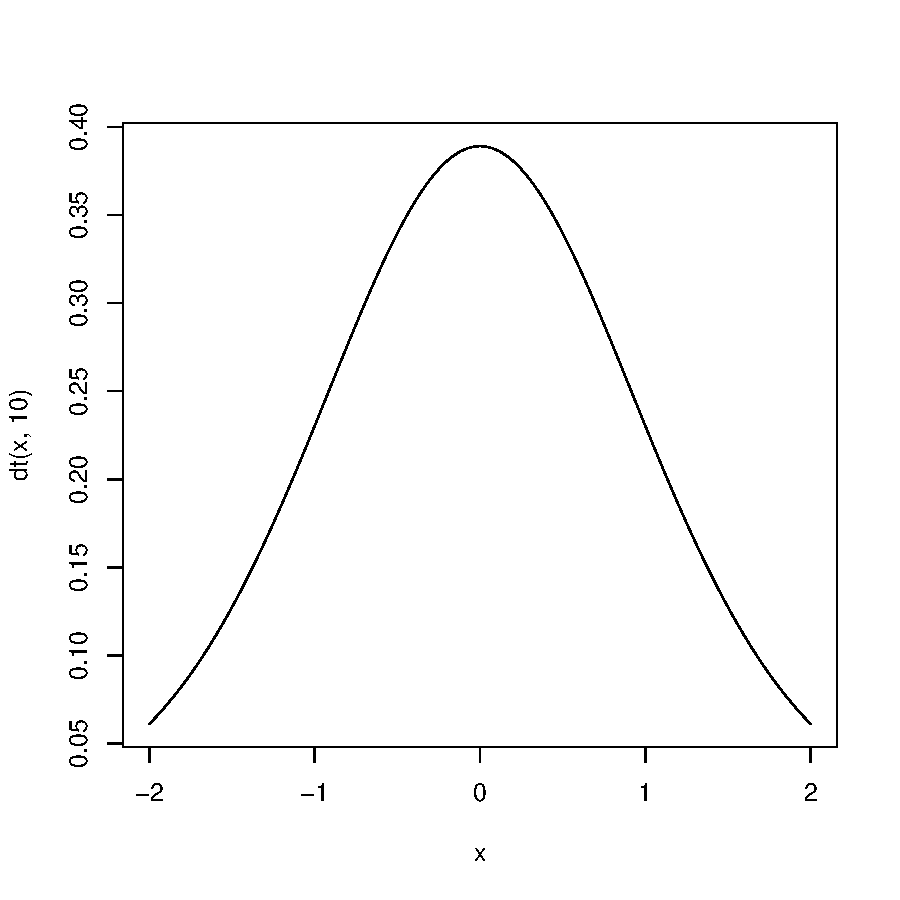
\includegraphics{RbookParte2-160}
\caption{Grafico della distribuzione di Student a 10 gradi di libert\`a. }
\label{fig:graficostudent1}
\end{center}
\end{figure}
Ricordiamo che la distribuzione di Student si usa in  particolare nei casi in cui la deviazione standard della popolazione $\sigma$  non \`e conosciuta e viene rimpiazzata  dalla deviazione standard campionaria  $S$, calcolata con un numero $N$ di dati e quindi con $N-1$ gradi di libert\`a. Quando per\`o il numero di dati si avvicina a 30 la curva di Student \`e praticamente sovrapposta a quella della distribuzione normale, come mostra il grafico~(\ref{fig:graficostudent}):

\begin{figure}[H]
\begin{center}
\begin{Schunk}
\begin{Sinput}
> curve(dnorm(x),-2,2,col=3)
> curve(dt(x,2),-2,2,col=1,add=T)
> curve(dt(x,25),-2,2,col=2,add=T)
> legend("topleft", c("df=2","df=25","normale"),pch=15,col=1:3);
\end{Sinput}
\end{Schunk}
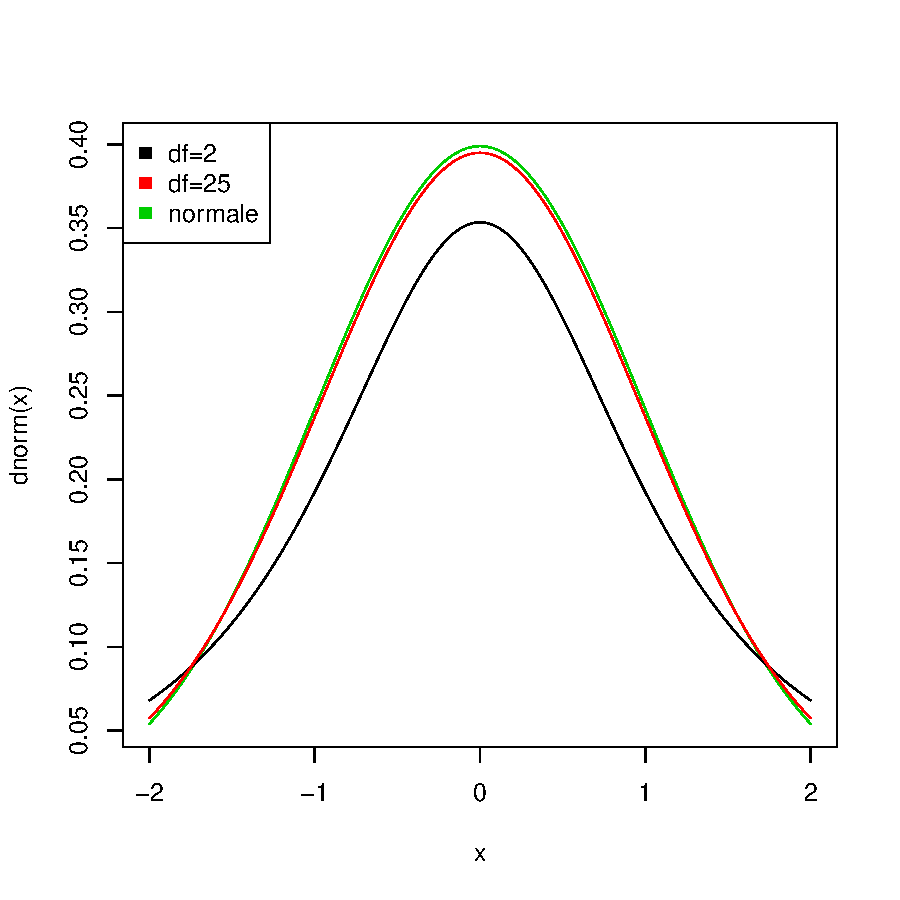
\includegraphics{RbookParte2-161}
\caption{Grafico della distribuzione di Student a 10 gradi di libert\`a. }
\label{fig:graficostudent}
\end{center}
\end{figure}
 \subsection
{Intervalli di confidenza e test di Student (dati non appaiati)}
La funzione di
\textsf{R} che esegue il test di Student nelle sue diverse forme \`e  \texttt{t.test}.   Nella sua forma pi\`u semplice

\begin{Schunk}
\begin{Sinput}
> x=1:20;  t.test(x)
\end{Sinput}
\begin{Soutput}
	One Sample t-test

data:  x
t = 7.9373, df = 19, p-value = 1.884e-07
alternative hypothesis: true mean is not equal to 0
95 percent confidence interval:
  7.731189 13.268811
sample estimates:
mean of x 
     10.5 
\end{Soutput}
\end{Schunk}
In assenza di ipotesi  \textsf{R} calcola il consuntivo $$t=\dfrac{M_N(X)-\mu}{S_X}\sqrt {N}$$
assumendo che sia $\mu=0$.
Possiamo anche eseguire specificare l'ipotesi sul valore di $\mu$:
\begin{Schunk}
\begin{Sinput}
> t.test(x,mu=7)
\end{Sinput}
\begin{Soutput}
	One Sample t-test

data:  x
t = 2.6458, df = 19, p-value = 0.01595
alternative hypothesis: true mean is not equal to 7
95 percent confidence interval:
  7.731189 13.268811
sample estimates:
mean of x 
     10.5 
\end{Soutput}
\end{Schunk}
Possiamo infine specificare l'ipotesi alternativa. Per esempio se l'ipotesi alternativa \`e
\texttt{\virgolette less\virgolette}  il risultato del test cambia completamente.
\begin{Schunk}
\begin{Sinput}
> t.test(x,mu=7, alternative="less")
\end{Sinput}
\begin{Soutput}
	One Sample t-test

data:  x
t = 2.6458, df = 19, p-value = 0.992
alternative hypothesis: true mean is less than 7
95 percent confidence interval:
     -Inf 12.78743
sample estimates:
mean of x 
     10.5 
\end{Soutput}
\end{Schunk}

In pratica ci viene fornito come $p$-value il valore dell'area sottesa dalla distribuzione di Student da $-\infty$ al valore di $t$ se l'ipotesi alternativa \`e  \texttt{\virgolette less\virgolette} e il valore dell'area sottesa dalla distribuzione di Student dal valore di $t$ a $+\infty$ se l'ipotesi alternativa \`e     \texttt{\virgolette greater\virgolette}  \subsection{Test di Student per dati appaiati}
Il test di Student per dati appaiati non \`e altro che un test di Student sulla differenza di 2 liste di dati di ugual lunghezza. Consideriamo ad esempio il confronto di 2 tecniche di misura applicate agli stessi campioni
\begin{Schunk}
\begin{Sinput}
> x<-c(1.46,2.22,2.84,1.97,1.13,2.35)
> y<-c(1.42,2.38,2.67,1.8,1.09,2.25)
\end{Sinput}
\end{Schunk}

Possiamo calcolare la differenza \texttt{x-y} ed applicare il test di Student oppure ottenere lo stesso risultato specificando l'opzione \texttt{paired=TRUE}
\begin{Schunk}
\begin{Sinput}
>  t.test(x,y,paired=TRUE)
\end{Sinput}
\begin{Soutput}
	Paired t-test

data:  x and y
t = 1.2, df = 5, p-value = 0.2839
alternative hypothesis: true difference in means is not equal to 0
95 percent confidence interval:
 -0.06852909  0.18852909
sample estimates:
mean of the differences 
                   0.06 
\end{Soutput}
\end{Schunk}

Il consuntivo   \texttt{t} cade entro la regione di accettazione del test.
\`E  possibile specificare il livello di fiducia da utilizzare per il test di Student come:

$$\texttt{conf.level}=\varia{numero}$$

Il comando completo di tutti i parametri  \`e quindi:
\begin{eqnarray*}
\texttt{t.test}(\varia{dati}_1,\varia{dati}_2,
\\
\texttt{paired=TRUE,conf.level}=\varia{valore})
\end{eqnarray*}
Ad esempio eseguiamo un $t$-test per dati appaiati, tra $x=(1,2,3,4)$ e $y=(3,2,4,5)$ con {\it confidence level} di 0.85. Scriveremo
\begin{Schunk}
\begin{Sinput}
> t.test(1:4,5:2,paired=TRUE,conf.level=0.85)
\end{Sinput}
\end{Schunk}
 Il consuntivo $t$ cade fuori dalla regione di accettazione proposta.

 \section{Test $\chi^2$  di indipendenza}

%code chunk
Consideriamo il seguente \emph{dataframe} che riporta le ambizioni di un gruppo di scolari americani
\begin{Schunk}
\begin{Sinput}
> data(kidinterest)
> str(kidinterest)
\end{Sinput}
\begin{Soutput}
'data.frame':	478 obs. of  11 variables:
 $ Gender     : Factor w/ 2 levels "boy","girl": 1 1 2 2 2 2 2 2 2 2 ...
 $ Grade      : int  5 5 5 5 5 5 5 5 5 5 ...
 $ Age        : int  11 10 11 11 10 11 10 10 10 10 ...
 $ Race       : Factor w/ 2 levels "Other","White": 2 2 2 2 2 2 2 2 2 2 ...
 $ Urban.Rural: Factor w/ 3 levels "Rural","Suburban",..: 1 1 1 1 1 1 1 1 1 1 ...
 $ School     : Factor w/ 9 levels "Brentwood Elementary",..: 4 4 4 4 4 4 4 4 4 4 ...
 $ Goals      : Factor w/ 3 levels "Grades","Popular",..: 3 2 2 2 2 2 2 1 3 3 ...
 $ Grades     : int  1 2 4 2 4 4 3 3 3 4 ...
 $ Sports     : int  2 1 3 3 2 2 4 4 2 3 ...
 $ Looks      : int  4 4 1 4 1 1 1 2 1 2 ...
 $ Money      : int  3 3 2 1 3 3 2 1 4 1 ...
\end{Soutput}
\end{Schunk}

Nella tabella le colonne che ci interessano al momento sono quelle che riguardano il sesso, gli obiettivi (scelti tra successo scolastico, capacit\`a sportiva e popolarit\`a) e la provenienza (colonne 1, 5  e 7). Nelle colonne dalla 8 alla 11 sono messi in ordine di importanza per il conseguimento della popolarit\`a  voti, sport, aspetto esteriore e denaro.
%codechunk
 
\begin{Schunk}
\begin{Sinput}
> interessi=kidinterest[,c(1,5,7)]
> head(interessi)
\end{Sinput}
\begin{Soutput}
  Gender Urban.Rural   Goals
1    boy       Rural  Sports
2    boy       Rural Popular
3   girl       Rural Popular
4   girl       Rural Popular
5   girl       Rural Popular
6   girl       Rural Popular
\end{Soutput}
\begin{Sinput}
> table(interessi)
\end{Sinput}
\begin{Soutput}
, , Goals = Grades

      Urban.Rural
Gender Rural Suburban Urban
  boy     21       51    45
  girl    36       36    58

, , Goals = Popular

      Urban.Rural
Gender Rural Suburban Urban
  boy     19       20    11
  girl    31       22    38

, , Goals = Sports

      Urban.Rural
Gender Rural Suburban Urban
  boy     26       18    16
  girl    16        4    10
\end{Soutput}
\end{Schunk}
Consideriamo per esempio le variabili provenienza e traguardi
\begin{Schunk}
\begin{Sinput}
> interessi2=kidinterest[,c(5,7)]
> tabella=table(interessi2)
> tabella
\end{Sinput}
\begin{Soutput}
           Goals
Urban.Rural Grades Popular Sports
   Rural        57      50     42
   Suburban     87      42     22
   Urban       103      49     26
\end{Soutput}
\end{Schunk}
 
Il test $\chi^2$  di indipendenza consente di  verificare se  due variabili sono indipendenti.
Se consideriamo le due variabili precedenti sesso e interessi.
\textsf{R}  dispone del comando \texttt{chisq.test},\index{\texttt{chisq.tst},test $\chi^2$}
dalla sintassi generale:$$\texttt{chisq.test}(\varia{tabella})$$

Nell'esempio
%code chunk
\begin{Schunk}
\begin{Sinput}
> data(studenti)
> str(studenti)
\end{Sinput}
\begin{Soutput}
'data.frame':	96 obs. of  9 variables:
 $ X   : int  1 2 3 4 5 6 7 8 9 10 ...
 $ Sex : Factor w/ 2 levels "F","M": 2 2 2 1 2 1 2 2 1 1 ...
 $ W   : num  86 53 64 61 64 51 78 55 59 52 ...
 $ H   : num  1.9 1.76 1.74 1.64 1.8 1.68 1.78 1.68 1.68 1.67 ...
 $ Eyes: Factor w/ 3 levels "azzurri","castani",..: 2 1 3 2 3 2 2 2 2 2 ...
 $ Hair: Factor w/ 3 levels "biondi","castani",..: 3 2 2 2 2 2 2 3 2 2 ...
 $ Sh  : int  48 42 41 39 42 38 42 40 38 39 ...
 $ hM  : num  1.58 1.7 1.63 1.65 1.56 1.6 1.65 1.56 1.58 1.65 ...
 $ hF  : num  1.82 1.6 1.8 1.78 1.75 1.75 1.75 1.7 1.83 1.7 ...
\end{Soutput}
\begin{Sinput}
> tabellaEH=table(studenti$Eyes,studenti$Hair)
> chisq.test(tabellaEH)
\end{Sinput}
\begin{Soutput}
	Pearson's Chi-squared test

data:  tabellaEH
X-squared = 5.9614, df = 4, p-value = 0.202
\end{Soutput}
\end{Schunk}
L'intervallo di accettazione dell'ipotesi (che ricordiamo \`e l'indipendenza) al 95\% di fiducia e 1 gradi di libert\`a \`e  $[0, 3.841]$, il consuntivo cade dentro, per cui l'ipotesi \`e accettata.
Per eliminare la correzione di Pearson si utilizza il parametro  \texttt{correct=FALSE}.
Ad esempio scriveremo:
%code chunk
\begin{Schunk}
\begin{Sinput}
> chisq.test(tabellaEH,correct=FALSE)
\end{Sinput}
\end{Schunk}

\subsection{Test $\chi^2$  di adeguamento}
Consideriamo una variabile aleatoria discreta con frequenza assoluta delle uscite racchiuse in una lista \texttt{data}. Ci si pone il problema di stabilire se tali frequenze sono compatibili con le probabilit\`a (riportate nella lista $p$).
\begin{Schunk}
\begin{Sinput}
> data<-c(2,3,4,5,6,7,8,9,10,11)
> prob<-c(5,20,5,10,5,15,5,10,10,15)
> sum(prob)
> chisq.test(data,p=prob,rescale.p=TRUE)
\end{Sinput}
\end{Schunk}
Si \`e usata qui la scelta \texttt{rescale.p=TRUE} in quanto la somma delle  probabilit\`a non era 1.
L'uscita del test riporta il valore del consuntivo $\chi^2$ i gradi di libert\`a ed il valore $p$.

\section{Distribuzione Binomiale}
Il coefficiente binomiale \`e definito come
\begin{equation*} \texttt{choose}(\varia{n},\varia{m})={n \choose m}=\dfrac{n!}{m!\times (n-m)!}\end{equation*}
Ad esempio
\begin{Schunk}
\begin{Sinput}
> choose(6,3)
\end{Sinput}
\begin{Soutput}
[1] 20
\end{Soutput}
\end{Schunk}
La distribuzione binomiale in \textsf{R} ha la sintassi $$\texttt{dbinom}(\varia{successi},\varia{prove},
\varia{probabilit\`a successo})$$ e fornisce la  probabilit\`a di ottenere nel corso di un certo numero di prove  il numero di successi indicato.\index{\texttt{dbinom}}
Ad esempio, nel lancio di un dado 10 volte, vogliamo determinare la  probabilit\`a che esca  \emph{esattamente} due volte il numero 4:
%codechunk
\begin{Schunk}
\begin{Sinput}
> dbinom(2,10,1/6)
\end{Sinput}
\begin{Soutput}
[1] 0.29071
\end{Soutput}
\end{Schunk}

La  probabilit\`a \`e circa del 29\%.


\begin{shaded}
\begin{description}
 \item{}conta i caratteri del tuo nome
\item{} vettore che contenga il quadrato dei primi 8 numeri pari
\item{}vettore che contenga la radice cubica dei primi 10 numeri naturali.
\item{}inserire in una matrice le coordinate 2D dei punti di un pentagono. Plot dei punti, come punti, come linee e come linee tratteggiate. Pi\`u arduo: riempimento della superficie
\item{}derivata di $x^3+x^2+2x+1$, plot della funzione e plot della derivata come due pannelli distinti in un grafico unico. hint: par(mfrow)
\end{description}
\end{shaded}
\begin{comment}

\section{Operatori condizionali e cicli}
with(rainforest, table(complete.cases(root), species))

Gli operatori condizionali valutano una condizione e in base alle risultanze assegnano valore ad una espressione

\begin{Schunk}
\begin{Sinput}
> b=1
> if (b==1) {print ("b vale 1");b=b+1}  else print(b);
\end{Sinput}
\begin{Soutput}
[1] "b vale 1"
\end{Soutput}
\end{Schunk}

Abbiamo poi i cicli \texttt{for} con la struttura
\begin{equation*}
\texttt{for} (i \texttt{it} \varia{sequenza}) \varia{esegui} B
\end{equation*}

\begin{Schunk}
\begin{Sinput}
> for (i in 1:10) print(i)#Somma di interi
> somma<-0
> for (i in  1:10) somma<-somma+i;somma
> #o anche come funzione
> somma<-function(n)
+ {somma<-0
+ for (i in  1:n) somma<-somma+i;somma
+ return(somma)}
\end{Sinput}
\end{Schunk}


\section{Funzioni di pi\`u variabili}
Finora abbiamo considerato funzioni di singola variabile. Una generalizzazione estremamente naturale consiste nel considerare funzioni di due o pi\`u variabili. Diamo alcuni esempi
\begin{enumerate}
\item{}
Calcolare la lunghezza del segmento che congiunge  due punti nel piano (distanza euclidea). Possiamo procedere con  una funzione di 4 numeri (le 2 coordinate dei 2 punti)
\begin{Schunk}
\begin{Sinput}
> dist<-function(x1,y1,x2,y2)
+ {dx<-(x2-x1)^2;dy<-(y2-y1)^2;return (sqrt(dx+dy))}
> dist(0,0,3,4)
\end{Sinput}
\begin{Soutput}
[1] 5
\end{Soutput}
\end{Schunk}
oppure possiamo generalizzare con una funzione che dipenda dai 2 vettori (e non direttamente dalle loro coordinate)
\begin{Schunk}
\begin{Sinput}
> dist<-function(x,y)
+ {return (sqrt(sum((x-y)^2)))}
\end{Sinput}
\end{Schunk}
\item{}: il massimo di due numeri
\begin{Schunk}
\begin{Sinput}
> massimo<-function(a,b)
+ if (a>b) return(a) else return(b)
\end{Sinput}
\end{Schunk}
Si noti che la condizione viene messa tra parentesi tonde.
\item{}: Il valore assoluto
\begin{Schunk}
\begin{Sinput}
> valoreassoluto<-function(a) if (a>0) return(a)  else return(-a)
\end{Sinput}
\end{Schunk}


\item{} Somma sino a $n$

\begin{Schunk}
\begin{Sinput}
> n=0;while (somma(n)<10000)
> n=n+1
> sommasinoa<-function(b) {i<-1;somma<-i;while (somma<=b)
+ {i=i+1;somma=somma+i}; return(i)}
\end{Sinput}
\end{Schunk}
\end{enumerate}


Generazione ricorsiva di successioni (successione di Fibonacci)
%code chunk
\begin{Schunk}
\begin{Sinput}
> fibonacci<-function(n)
+ {f=0;f[1]<-1;f[2]<-1;for (i in 3:n) {f[i]<-f[i-1]+f[i-2]};return(f[n])}
\end{Sinput}
\end{Schunk}

\section{R  Output su file}

\begin{Schunk}
\begin{Sinput}
> cat("TITLE extra line", "2 4 5 7", "11 13 17", file="ex.data", sep="\n",append=T)
> cat("TITLE extra line", "2 4 5 7", "11 13 17", sep="\n")
\end{Sinput}
\end{Schunk}
\begin{Schunk}
\begin{Sinput}
> print()
> read.delim
>  aggregate
> 
\end{Sinput}
\end{Schunk}

\chapter{Statistica II parte}
%\section{Simulazioni e statistica Bayesiana}
Uno degli usi rilevanti a fini statistici dei computer  \`e la possibilit\`a di stimare attraverso simulazioni probabilit\`a difficili da calcolare teoricamente.
\begin{shaded}\begin{description}
\item{\bf Estrazioni da un'urna. }Supponiamo 2 palle siano estratte da un'urna contenente 6 palle rosse e 2 verdi.
Simuliamo due estrazioni e consideriamo gli eventi:
\begin{itemize}
\item{}$A$ = {la prima palla  \`e rossa}
\item{}$B$ = {la seconda palla \`e rossa}
\end{itemize}
Determinare le probabilit\`a
$P(A)$, $P(B)$,
$P(A\wedge B)$, $P(A \mid B)$,
$P(B \mid A)$.
Eseguire poi la simulazione 1000 volte e verificare che le stime frequentiste si avvicinano ai valori teorici. Si usi la funzione \texttt{replicates}.\index{\texttt{replicates}}
Gli ultimi due punti richiedono opportuni accorgimenti.
\item{\bf Simulazione del problema di  Monthy Hall.}
Il problema di Monthy Hall ricalca una trasmissione televisiva americana. Immaginate di avere tre porte chiuse dietro alle quali si nascondono 2 capre e un premio, una Ferrari per esempio. L'ospite deve scegliere una porta; effettuata tale scelta il presentatore (che conosce cosa si nasconde dietro alle 3 porte) apre una porta mostrando una capra e d\`a all'ospite la scelta se attenersi alla scelta originale o cambiare porta. Cosa fareste se foste voi l'ospite?
\end{description}
\end{shaded}
Come si pu\`o simulare il problema di Monthy Hall?
Iniziamo a disporre gli oggetti e a fare la nostra scelta
%code chunk
\begin{Schunk}
\begin{Sinput}
> set.seed(12)
> (sample(c("capra","capra","ferrari"))->posizione)
\end{Sinput}
\begin{Soutput}
[1] "capra"   "capra"   "ferrari"
\end{Soutput}
\begin{Sinput}
> (scelta<-sample(1:3,1))
\end{Sinput}
\begin{Soutput}
[1] 1
\end{Soutput}
\end{Schunk}
A questo punto  il presentatore deve aprire una porta,
\begin{Schunk}
\begin{Sinput}
> (ammessa<-(1:3)[-unique(c(scelta,which(posizione=="ferrari")))])
\end{Sinput}
\begin{Soutput}
[1] 2
\end{Soutput}
\begin{Sinput}
> if(length(ammessa)==1)
+ presentatore<-ammessa else presentatore=sample(ammessa,1)
\end{Sinput}
\end{Schunk}
Ripetiamolo ora 1000 volte
\begin{Schunk}
\begin{Sinput}
> replicate(1000,{
+ sample(c("capra","capra","ferrari"))->dietro;
+ scelta=sample(1:3,1);
+ ammessi=(1:3)[-unique(c(scelta,which(
+ dietro=="ferrari")))];
+ if(length(ammessi)==1) {presentatore=ammessi} else {presentatore=sample(ammessi,1)};
+ c(dietro[scelta],dietro[-c(scelta,presentatore)])})->risultato
> table(risultato[1,]);table(risultato[2,]);
\end{Sinput}
\end{Schunk}

\section{Analisi della Varianza (ANOVA)}
L'analisi della varianza diviene estremamente semplice da eseguire con \textsf{R}  a patto di \emph{preparare} i dati in modo opportuno.
Consideriamo il seguente esempio tratto dal libro di Snedecor \cite{snedecor} in cui si considera l'assorbimento di grasso durante la cottura di 24 \emph{donuts}. Si esaminano 4 tipi di grasso di cottura 4 e la cottura di 6 \emph{donuts} per ciascun tipo. Inseriamo nella lista  $x$ il gruppo di appartenenza e nella lista $y$ le quantit\`a di grasso assorbito.
\begin{Schunk}
\begin{Sinput}
> x<-rep(1:4,each=6)
> factor(x)->x
> x<-gl(4,6);x
\end{Sinput}
\begin{Soutput}
 [1] 1 1 1 1 1 1 2 2 2 2 2 2 3 3 3 3 3 3 4 4 4 4 4 4
Levels: 1 2 3 4
\end{Soutput}
\begin{Sinput}
> y<-c(15,20,22,23,25,26,80,90,76,56,5,
+ 43,23,45,67,89,87,65,43,23,45,10,11,23)
> tabelladati=data.frame(y,x)
> tabelladati
\end{Sinput}
\begin{Soutput}
    y x
1  15 1
2  20 1
3  22 1
4  23 1
5  25 1
6  26 1
7  80 2
8  90 2
9  76 2
10 56 2
11  5 2
12 43 2
13 23 3
14 45 3
15 67 3
16 89 3
17 87 3
18 65 3
19 43 4
20 23 4
21 45 4
22 10 4
23 11 4
24 23 4
\end{Soutput}
\end{Schunk}
Il comando  \texttt{tapply} consente di applicare una funzione (in questo caso la media) alla lista  $y$ in base alla ripartizione indicata da $x$.
$$\texttt{tapply}(y,x,\texttt{mean})$$
In questo caso
\begin{Schunk}
\begin{Sinput}
> tapply(y,x,mean)
\end{Sinput}
\begin{Soutput}
       1        2        3        4 
21.83333 58.33333 62.66667 25.83333 
\end{Soutput}
\end{Schunk}
In modo simile all'uso del simbolo $\sim$ visto nei comandi per la regressione lineare il comando
$$\texttt{boxplot}(y\sim x,data=tabella)$$
consente il tracciamento di un \emph{boxplot} comparativo.
\begin{Schunk}
\begin{Sinput}
> boxplot(y~x,data=tabelladati)
\end{Sinput}
\end{Schunk}
\begin{figure}[htbp]
\begin{center}
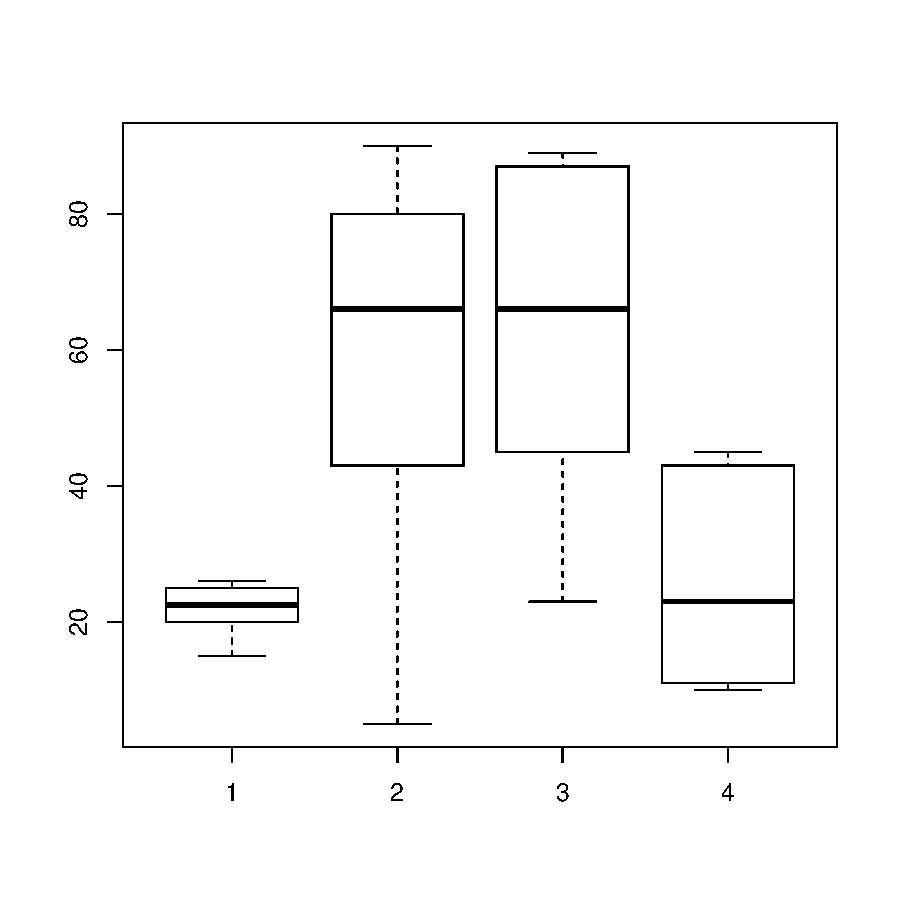
\includegraphics{RbookParte2-192}
\caption{Boxplot comparativo di 4 tipi di grasso di cottura.}
\label{datiist}
\end{center}
\end{figure}
In modo analogo
 <<echo=TRUE>>=
anova(lm(y~x))

fornisce il risultato dell'analisi della varianza.



\section{Test $\chi^2$  di indipendenza}

%code chunk
\begin{Schunk}
\begin{Sinput}
> read.table("../filedati/PopularKids.html",skip=39,header=T,nrow=478,sep="\t")->kidinterest
\end{Sinput}
\end{Schunk}
Il test $\chi^2$  di indipendenza consente di  verificare se  due variabili sono indipendenti.
Se consideriamo le due variabili precedenti sesso e interessi.
\textsf{R}  dispone del comando \texttt{chisq.test},\index{\texttt{chisq.tst},test $\chi^2$} dalla sintassi generale:$$\texttt{chisq.test}(\varia{tabella})$$

Nell'esempio
%code chunk
\begin{Schunk}
\begin{Sinput}
> tabellaEH=table(studenti$Eyes,studenti$Hair)
> chisq.test(tabellaEH)
\end{Sinput}
\begin{Soutput}
	Pearson's Chi-squared test

data:  tabellaEH
X-squared = 5.9614, df = 4, p-value = 0.202
\end{Soutput}
\end{Schunk}
L'intervallo di accettazione dell'ipotesi (che ricordiamo \`e l'indipendenza) al 95\% di fiducia e 1 gradi di libert\`a \`e  $[0, 3.841]$, il consuntivo cade dentro, per cui l'ipotesi \`e accettata.
Per eliminare la correzione di Pearson si utilizza il parametro  \texttt{correct=FALSE}.
Ad esempio scriveremo:
%code chunk
\begin{Schunk}
\begin{Sinput}
> chisq.test(tabellaEH,correct=FALSE)
\end{Sinput}
\end{Schunk}

\subsection{Test $\chi^2$  di adeguamento}
Consideriamo una variabile aleatoria discreta con frequenza assoluta delle uscite racchiuse in una lista \texttt{data}. Ci si pone il problema di stabilire se tali frequenze sono compatibili con le probabilit\`a (riportate nella lista $p$).
\begin{Schunk}
\begin{Sinput}
> data<-c(2,3,4,5,6,7,8,9,10,11)
> prob<-c(5,20,5,10,5,15,5,10,10,15)
> sum(prob)
> chisq.test(data,p=prob,rescale.p=TRUE)
\end{Sinput}
\end{Schunk}
Si \`e usata qui la scelta \texttt{rescale.p=TRUE} in quanto la somma delle  probabilit\`a non era 1.
L'uscita del test riporta il valore del consuntivo $\chi^2$ i gradi di libert\`a ed il valore $p$.

\section{Distribuzione Binomiale}
Il coefficiente binomiale \`e definito come
\begin{equation*} \texttt{choose}(\varia{n},\varia{m})={n \choose m}=\dfrac{n!}{m!\times (n-m)!}\end{equation*}
Ad esempio
\begin{Schunk}
\begin{Sinput}
> choose(6,3)
\end{Sinput}
\begin{Soutput}
[1] 20
\end{Soutput}
\end{Schunk}
La distribuzione binomiale in \textsf{R} ha la sintassi $$\texttt{dbinom}(\varia{successi},\varia{prove},
\varia{probabilit\`a successo})$$ e fornisce la  probabilit\`a di ottenere nel corso di un certo numero di prove  il numero di successi indicato.\index{\texttt{dbinom}}
Ad esempio, nel lancio di un dado 10 volte, vogliamo determinare la  probabilit\`a che esca  \emph{esattamente} due volte il numero 4:
%codechunk
\begin{Schunk}
\begin{Sinput}
> dbinom(2,10,1/6)
\end{Sinput}
\begin{Soutput}
[1] 0.29071
\end{Soutput}
\end{Schunk}

La  probabilit\`a \`e circa del 29\%.


\section{Distribuzione di Fisher}

La distribuzione di Fisher \`e indicata in \textsf{R} con la lettera \texttt{f}. Per tracciare il grafico della densit\`a con gradi di libert\`a $\nu_1$ e $\nu_2$ basta scrivere
\begin{Schunk}
\begin{Sinput}
> curve(df(x,3,10),0,5)
\end{Sinput}
\end{Schunk}
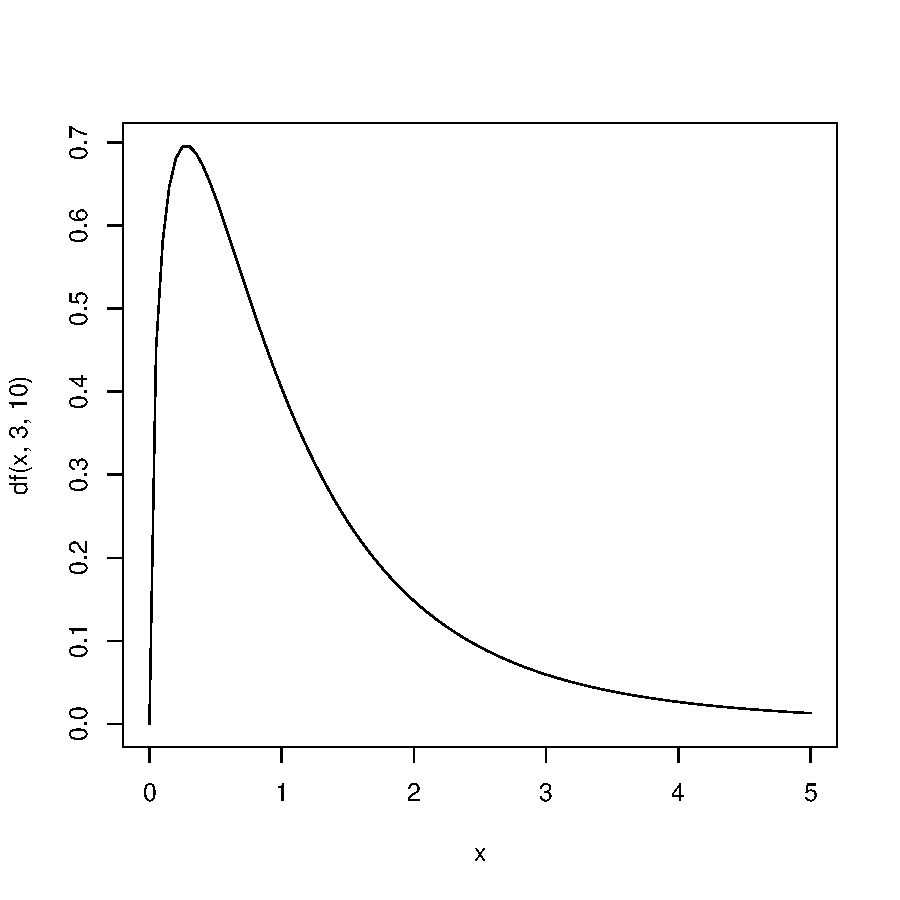
\includegraphics{RbookParte2-199}
ottenendo il grafico
\begin{figure}[htbp]
\begin{center}
\begin{Schunk}
\begin{Sinput}
> curve(df(x,3,10),0,5)
\end{Sinput}
\end{Schunk}
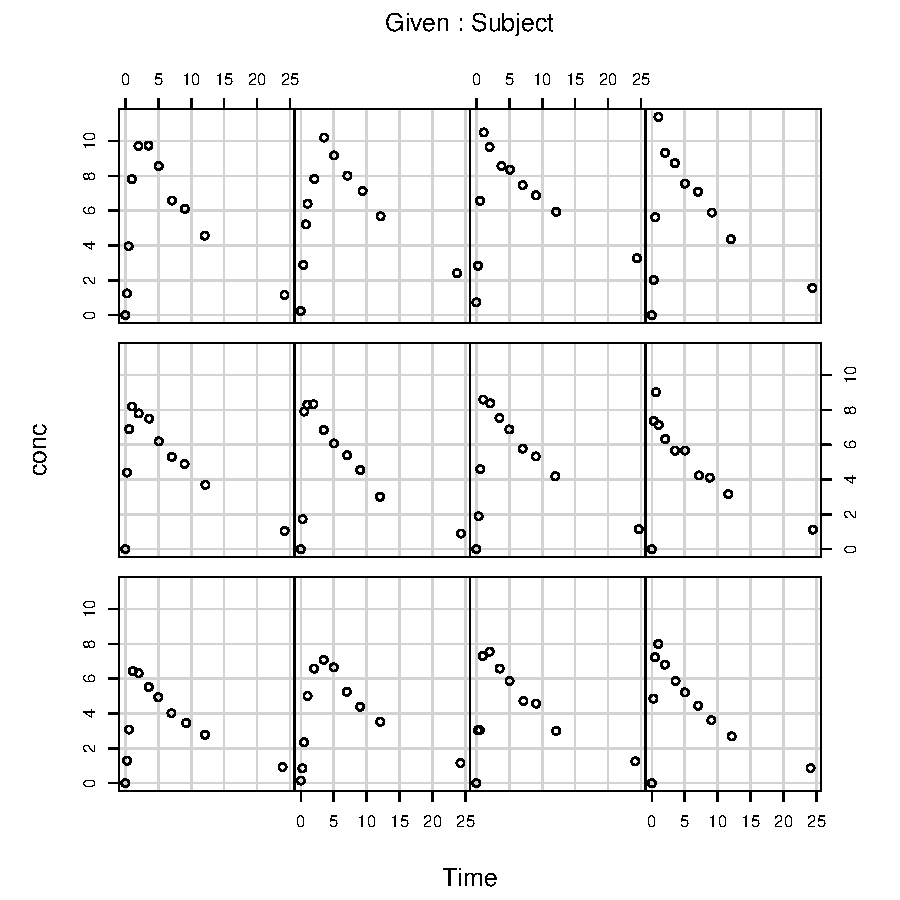
\includegraphics{RbookParte2-200}
\caption{Distribuzione di Fisher.}
\label{fig:fisher}
\end{center}
\end{figure}.

Dobbiamo solo definire $x$, $df1$ e $df2$, gradi di libert\`a per poi applicare \texttt{df},\texttt{qf}, \texttt{rf} come visto per le distribuzioni precedenti.
Per esempio per ottenere il valore della funzione inversa  per $x=0.9$ e $df1=3$ e $df2=4$ scriveremo:
\begin{Schunk}
\begin{Sinput}
> qf(0.9,3,4)
\end{Sinput}
\begin{Soutput}
[1] 4.19086
\end{Soutput}
\end{Schunk}


\section{Tabelle di contingenza}
Il comando
$\texttt{table}$ applicato ad un lista contenente valori di una singola variabile nominale conta le frequenze di ciascuna livello, se applicato ad un \emph{dataframe} di $n$  variabili conta le occorrenze di  ciascuna combinazione di livelli possibile ($2^n$ se le variabili sono dicotomiche). Per esempio se consideriamo il \emph{dataframe}  \texttt{studenti}  possiamo creare una tabella dei colori degli occhi e dei capelli
%code chunk
\begin{Schunk}
\begin{Sinput}
> tabellaEH=table(studenti$Eyes,studenti$Hair)
\end{Sinput}
\end{Schunk}






\section{Farmacocinetica e modelli non lineari}

Dopo la somministrazione, un farmaco viene distribuito alle regioni del corpo accessibili.
Se consideriamo questo evento istantaneo, il corpo pu\`o qui essere considerato un contenitore omogeneo del farmaco, e la cinetica di diffusione pu\`o essere modellata con un modello a singolo compartimento aperto.
Quest'ultimo termine significa che il contenuto del compartimento non \`e confinato nel compartimento.
Se invece la diffusione non \`e istantanea e il contenuto arriva al siero secondo un modello di decrescita malthusiana,  il sistema  pu\`o essere modellato come un sistema a due compartimenti aperti.

Il dataset \texttt{Theoph} contiene 11 misure di concentrazione (a diversa tempistica) per ciascuno dei 12 soggetti sottoposti a somministrazione orale di teofillina.
\begin{Schunk}
\begin{Sinput}
> head(Theoph)
\end{Sinput}
\begin{Soutput}
  Subject   Wt Dose Time  conc
1       1 79.6 4.02 0.00  0.74
2       1 79.6 4.02 0.25  2.84
3       1 79.6 4.02 0.57  6.57
4       1 79.6 4.02 1.12 10.50
5       1 79.6 4.02 2.02  9.66
6       1 79.6 4.02 3.82  8.58
\end{Soutput}
\end{Schunk}
Diamo una prima occhiata ai dati con il comando \texttt{coplot}, ovvero {\it conditioning plot}.  Il comando richiede un modello/formula, del tipo $(x y|a)$, che significa $x$ versus $y$ dato $a$ (ecco perch? conditioning). Se le variabili rispetto alle quali riportare il grafico sono pi\`u di una, basta aggiungere tra esse un segno $+$.
\begin{Schunk}
\begin{Sinput}
> require(graphics)
> coplot(conc ~ Time | Subject, data = Theoph, show.given = FALSE)
\end{Sinput}
\end{Schunk}
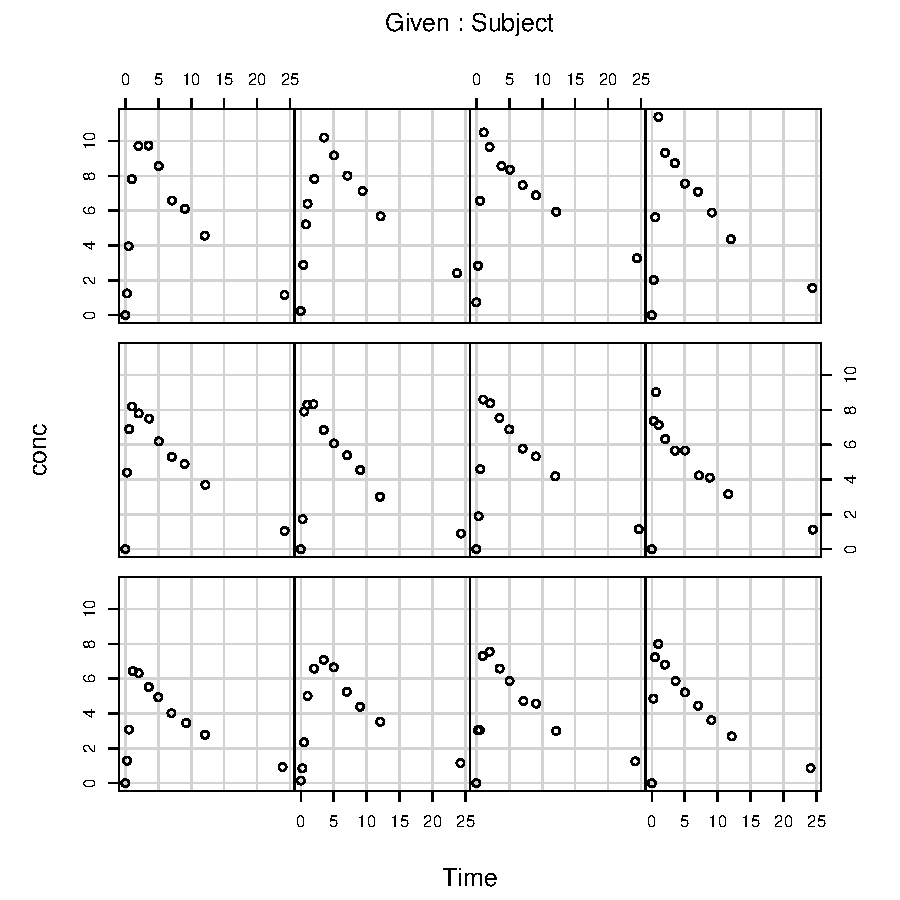
\includegraphics{RbookParte2-205}

Selezioniamo ora il paziente 4, lo possiamo fare note le righe che esso occupa nel dataframe oppure selezionando per un preciso valore della variabile Subject.

\begin{Schunk}
\begin{Sinput}
> Theoph.4 <- subset(Theoph, Subject == 4)
\end{Sinput}
\end{Schunk}
\subsection{Regressione non lineare}
In statistica, una regressione non lineare \`e una forma di regressione in cui i dati osservati sono modellati da una funzione che non \`e una combinazione lineare dei parametri e che dipende da una o pi\`u  variabili indipendenti.

Il comando \texttt{nls} determina le stime dei parametri di un modello non lineare con il metodo dei minimi quadrati (ponderati).
Se consideriamo un modello a 2 compartimenti aperti del primo ordine descritto da sistema di equazioni differenziali
\begin{equation}\begin{cases}
x'(t)&= -k_a x(t)\\
y'(t)&= k_a x(t)-k_e y(t)
\end{cases}
\end{equation}
troviamo la soluzione
\begin{equation}
\begin{cases}
x(t)=&x_0 e^{-k_a t}\\
y(t) =&x_0 k_a  \frac{e^{-k_e t} - e^{-k_a t}}{k_a-k_e}
\end{cases}
 \end{equation}
In particolare la funzione \texttt{SSfol} in \textsf{R} consente di descrivere una cinetica del primo ordine per il modello a proposto. Essa infatti restituisce i logaritmi dei parametri di eliminazione, assorbimento e  \emph{clearance} (\texttt{lKe, lKa, lCl}).
L'uso \`e il seguente
\begin{equation*}\texttt{SSfol(Dose, input, lKe, lKa, lCl})
\end{equation*}
dove \texttt{Dose}  rappresenta la dose iniziale,  \texttt{input} \`e un vettore numerico con il quale valutiamo il modello. \texttt{lKe} \`e un parametro numerico che rappresenta il logaritmo naturale della costante velocit\`a di eliminazione. \texttt{lKa} \`e un parametro numerico che rappresenta il logaritmo naturale della costante velocit\`a di assorbimento mentre  \texttt{lCl} \`e un parametro numerico che rappresenta il logaritmo naturale  della \emph{clearance}.
Proviamo ad utilizzare il comando \texttt{SSfol}, e inseriamo il risultato della regressione nella variabile \texttt{fm1} (modello 1).
%code chunk
\begin{Schunk}
\begin{Sinput}
> fm1 <- nls(conc ~ SSfol(Dose, Time, lKe, lKa, lCl), data = Theoph.4)
\end{Sinput}
\end{Schunk}
Osserviamo \texttt{fm1},  con il comando \texttt{summary}
\begin{Schunk}
\begin{Sinput}
> summary(fm1)
\end{Sinput}
\begin{Soutput}
Formula: conc ~ SSfol(Dose, Time, lKe, lKa, lCl)

Parameters:
    Estimate Std. Error t value Pr(>|t|)    
lKe  -2.4365     0.2257 -10.797 4.77e-06 ***
lKa   0.1583     0.2297   0.689     0.51    
lCl  -3.2861     0.1448 -22.695 1.51e-08 ***
---
Signif. codes:  
0 ‘***’ 0.001 ‘**’ 0.01 ‘*’ 0.05 ‘.’ 0.1 ‘ ’ 1

Residual standard error: 0.8465 on 8 degrees of freedom

Number of iterations to convergence: 7 
Achieved convergence tolerance: 2.969e-06
\end{Soutput}
\end{Schunk}

Ora riportiamo il grafico delle osservazioni per il soggetto 4 su un grafico singolo:

\begin{Schunk}
\begin{Sinput}
> options(width=40)
> plot(conc ~ Time, data = Theoph.4,
+ xlab = "tempo dalla somministazione (ore)",
+  ylab = "Concentrazione di Teofillina(mg/L)",
+ main = "Concentrazioni osservate e modello", sub = "Soggetto 4",
+ las = 1, col = 4)
\end{Sinput}
\end{Schunk}
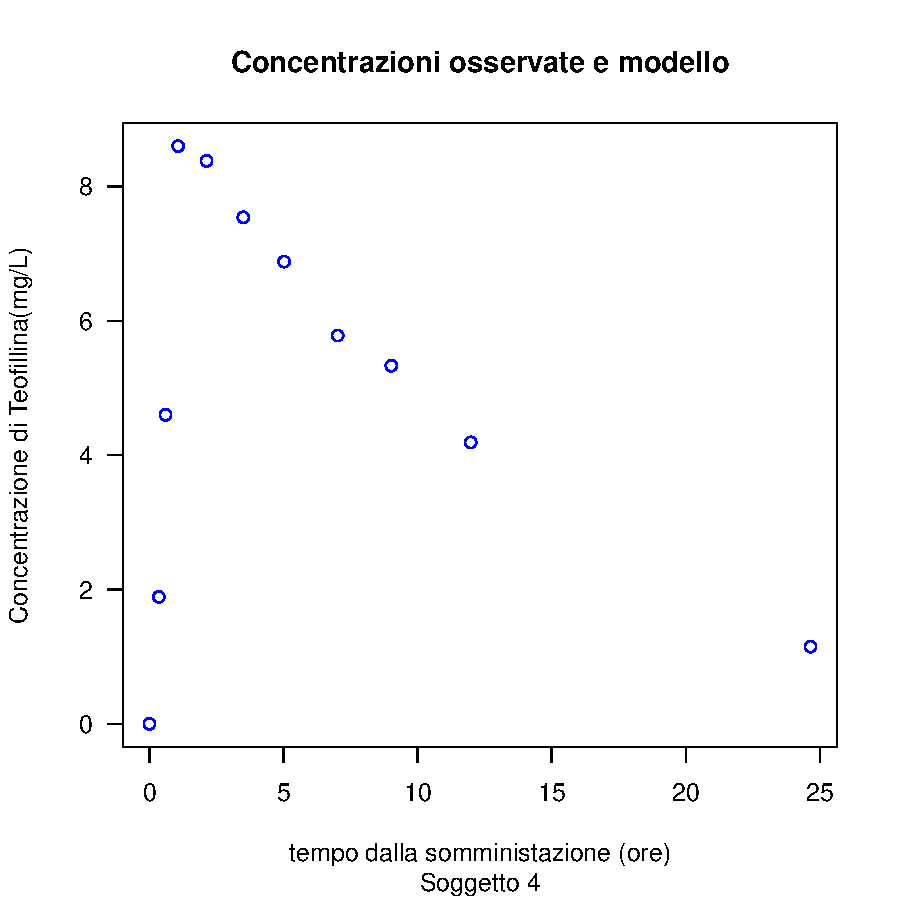
\includegraphics{RbookParte2-209}

Si pu\`o ora sovrapporre la curva ottenuta con il modello al grafico attuale.
Per prima cosa definiamo i possibili valori di $x$.

\begin{Schunk}
\begin{Sinput}
> xvals <- seq(0, par("usr")[2], length.out = 55)
\end{Sinput}
\end{Schunk}

dove \texttt{par(usr)}  \`e un ottimo modo per conoscere l'estensione di una delle dimensioni della finestra grafica. A tali valori di $x$ vengono associati i corrispettivi valori $y$ della curva, ottenuti con il comando \texttt{predict}, che utilizza diversi metodi predittivi noti i valori delle costanti del modello ed i valori di $x$. In questo caso il tempo (la nostra $x$)  \`e  uguale ai valori \texttt{xvars} appena calcolati.

\begin{Schunk}
\begin{Sinput}
> plot(conc ~ Time, data = Theoph.4,
+ xlab = "tempo dalla somministazione (ore)",
+ ylab = "Concentrazione di Teofillina(mg/L)",
+ main = "Concentrazioni osservate e modello", sub = "Soggetto 4",
+ las = 1, col = 4)
> lines(xvals, predict(fm1, newdata = list(Time = xvals)), col = 4)
\end{Sinput}
\end{Schunk}
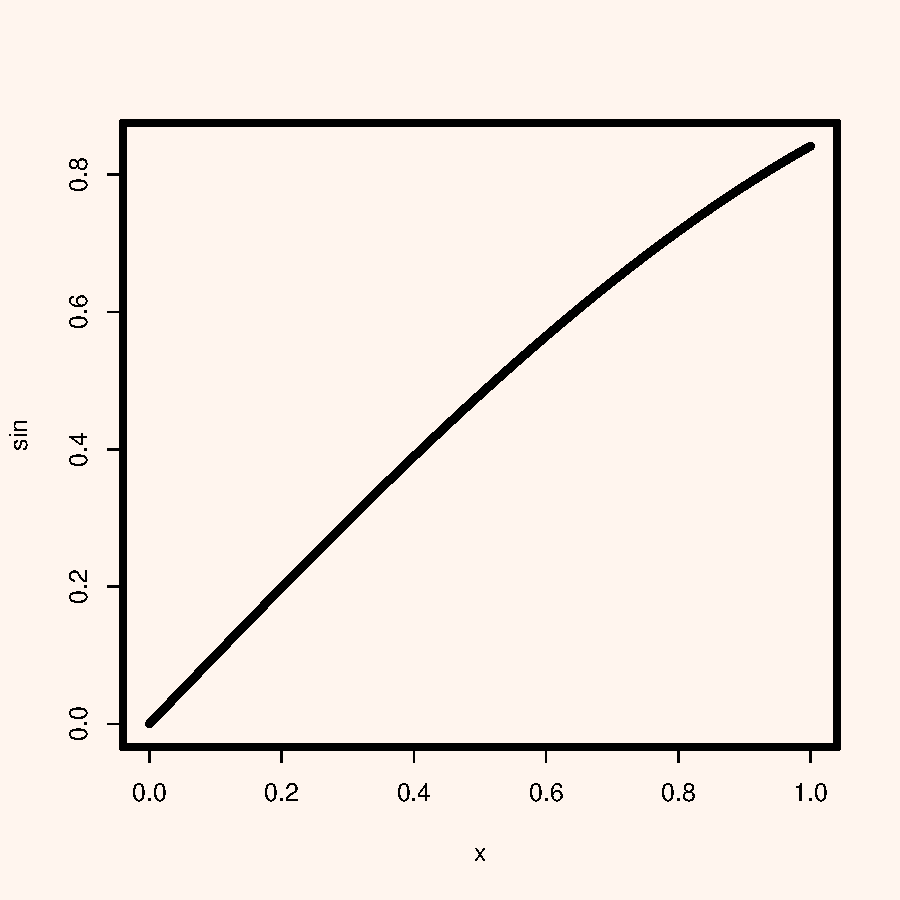
\includegraphics{RbookParte2-211}


\section{QQPlot
normality test}
\chapter{Grafica}
Il sistema grafico di \textsf{R} si compone di 3 parti: grafica di alto livello che produce grafici completi (per esempio \texttt{plot}, \texttt{curve}), grafica di basso livello che aggiunge elementi a grafici preesistenti (\texttt{text}, \texttt{abline}) e funzioni che lavorano interattivamente con grafici (ad esempio \texttt{locator()} e \texttt{identify()}).
\cite{murrell}.
A fianco della grafica tradizionale (gestita dal pacchetto \texttt{graphics}) esistono sistemi non tradizionali cui si pu\`o accedere attraverso il pacchetto \texttt{grid}. \index{\texttt{grid}}
In questo capitolo ci dedicheremo essenzialmente ad inquadrare la grafica tradizionale e daremo alcuni cenni sulla grafica non tradizionale.
\section{Le \emph{device} grafiche}
Le \emph{device} grafiche consentono di realizzare grafici di \textsf{R} su file di diversi formati (per esempio \texttt{.pdf}, \texttt{.ps}, \texttt{.bmp},\texttt{ .jpeg}, \texttt{.tiff}).
Il grafico anzich\'e essere  visualizzato a schermo, pu\`o quindi essere salvato direttamente in diversi formati. Per esempio il comando
\begin{Schunk}
\begin{Sinput}
> pdf(file = "miografico.pdf")
> plot(1:10)
> dev.off()
\end{Sinput}
\end{Schunk}
genera un file \texttt{.pdf} di nome \texttt{miografico} nella \emph{working directory}.
Se omettiamo il nome avremo il nome di defaults \texttt{Rplots}.
Per particolari \emph{device}  (per esempio \text{pdf}) la stampa su \emph{file} pu\`o occupare diverse pagine e quindi si possono inserire in un unico file diversi grafici.
Occorre ricordarsi di chiudere la \emph{device} al termine della produzione grafica con il comando \texttt{dev.off()}.
Il grafico sar\`a direttamente prodotto nel file indicato, dunque non si vedranno finestre grafiche e  apparir\`a  a schermo solo  un messaggio di avvenuta realizzazione del file una volta che la
\emph{device} viene chiusa.
La sintassi generica richiede dunque
\begin{enumerate}
\item{}Apertura della \emph{device} (definendone il nome, la dimensione
ed altri parametri non obbligatori, come la risoluzione)
\item{} Comandi grafici.
\item{} Chiusura della \emph{device}.
\end{enumerate}
Nota: le \emph{device} possono presentare piccole variazioni nei parametri, in particolare nei loro nomi. Un esempio: il nome del file in \texttt{png} \`e  definito dal parametro \texttt{filename=}, mentre nella device pdf \`e definito dal parametro \texttt{file=}. Consultare l'\emph{help} prima di utilizzarle non \`e  una cattiva idea. Tutti i parametri grafici visti valgono allo stesso modo per le \emph{device}.

\section{Lo stato grafico}
Ogni \emph{device} grafica mantiene uno stato grafico che viene consultato da \textsf{R} ogni volta che la \emph{device} viene usata. Lo stato grafico consiste in una serie di parametri specificabili con il comando \texttt{par}, nella forma
\begin{equation*}\texttt{par}(\varia{parametro}_1=\texttt{val}_1,\ldots)
\end{equation*}
Tecnicamente \texttt{par()} \`e una funzione  che restituisce una lista.
I parametri grafici specificabili con \texttt{par} sono ottenibili con il comando
\begin{Schunk}
\begin{Sinput}
> options(width=55)
> class(par())
\end{Sinput}
\begin{Soutput}
[1] "list"
\end{Soutput}
\begin{Sinput}
> names(par())
\end{Sinput}
\begin{Soutput}
 [1] "xlog"      "ylog"      "adj"       "ann"      
 [5] "ask"       "bg"        "bty"       "cex"      
 [9] "cex.axis"  "cex.lab"   "cex.main"  "cex.sub"  
[13] "cin"       "col"       "col.axis"  "col.lab"  
[17] "col.main"  "col.sub"   "cra"       "crt"      
[21] "csi"       "cxy"       "din"       "err"      
[25] "family"    "fg"        "fig"       "fin"      
[29] "font"      "font.axis" "font.lab"  "font.main"
[33] "font.sub"  "lab"       "las"       "lend"     
[37] "lheight"   "ljoin"     "lmitre"    "lty"      
[41] "lwd"       "mai"       "mar"       "mex"      
[45] "mfcol"     "mfg"       "mfrow"     "mgp"      
[49] "mkh"       "new"       "oma"       "omd"      
[53] "omi"       "page"      "pch"       "pin"      
[57] "plt"       "ps"        "pty"       "smo"      
[61] "srt"       "tck"       "tcl"       "usr"      
[65] "xaxp"      "xaxs"      "xaxt"      "xpd"      
[69] "yaxp"      "yaxs"      "yaxt"      "ylbias"   
\end{Soutput}
\end{Schunk}
Per verificare lo stato grafico corrente basta scrivere \texttt{par()}. Per conoscere lo stato grafico di un particolare parametro basta scrivere $\texttt{par("\varia{nome parametro})"}$.
Ad esempio il parametro \texttt{bg} si riferisce al colore dello sfondo del grafico di default trasparente, mentre il parametro \texttt{lwd} si riferisce allo spessore delle linee.
Per cambiare i default dei due parametri
\begin{Schunk}
\begin{Sinput}
> oldpar<-par(bg="seashell1","lwd"=5)
> plot(sin)
\end{Sinput}
\end{Schunk}
Qui contestualmente alla ridefinizione abbiamo salvato (con il nome \texttt{oldpar}) la versione corrente dei parametri per poterli eventualmente ripristinare in seguito.
\begin{figure}\begin{center}
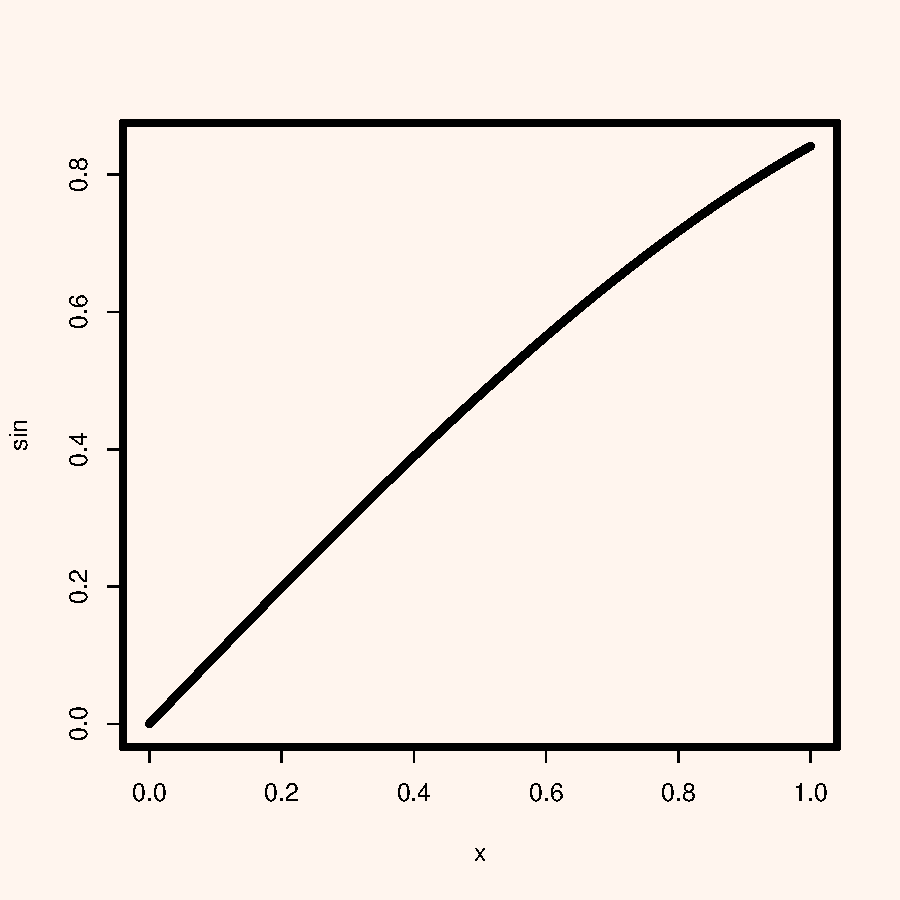
\includegraphics{RbookParte2-215}
\caption{esempio di utilizzo di \texttt{par()}
}
\label{parbg}
\end{center}
\end{figure}
ottenendo la figura~\ref{parbg}.
Si noti che si possono riesumare i valori precedenti
\begin{Schunk}
\begin{Sinput}
> par("bg")
\end{Sinput}
\begin{Soutput}
[1] "seashell"
\end{Soutput}
\begin{Sinput}
> par(oldpar)
> par("bg")
\end{Sinput}
\begin{Soutput}
[1] "transparent"
\end{Soutput}
\end{Schunk}
\section{Elementi grafici di base}
\subsection{Costruzione di grafici multipli}
In questo capitolo disegneremo diversi grafici;  consideriamo preliminarmente la possibilit\`a di affiancarli in riga e in colonna, sia per ragioni di spazio che di chiarezza.
Per costruire tabelle di grafici in una finestra unica si usa il comando
\begin{equation*}
\texttt{par(mfrow=c}(\varia{nrighe},\varia{ncolonne}))
\end{equation*}
Per esempio  con una riga e due colonne
\begin{Schunk}
\begin{Sinput}
> par(mfrow=c(1,2))
> plot(iris[,1],iris[,2])
> plot(iris[,3],iris[,4])
\end{Sinput}
\end{Schunk}
otteniamo i grafici affiancati della figura \ref{graficiaffiancati}.
\begin{figure}
\begin{center}
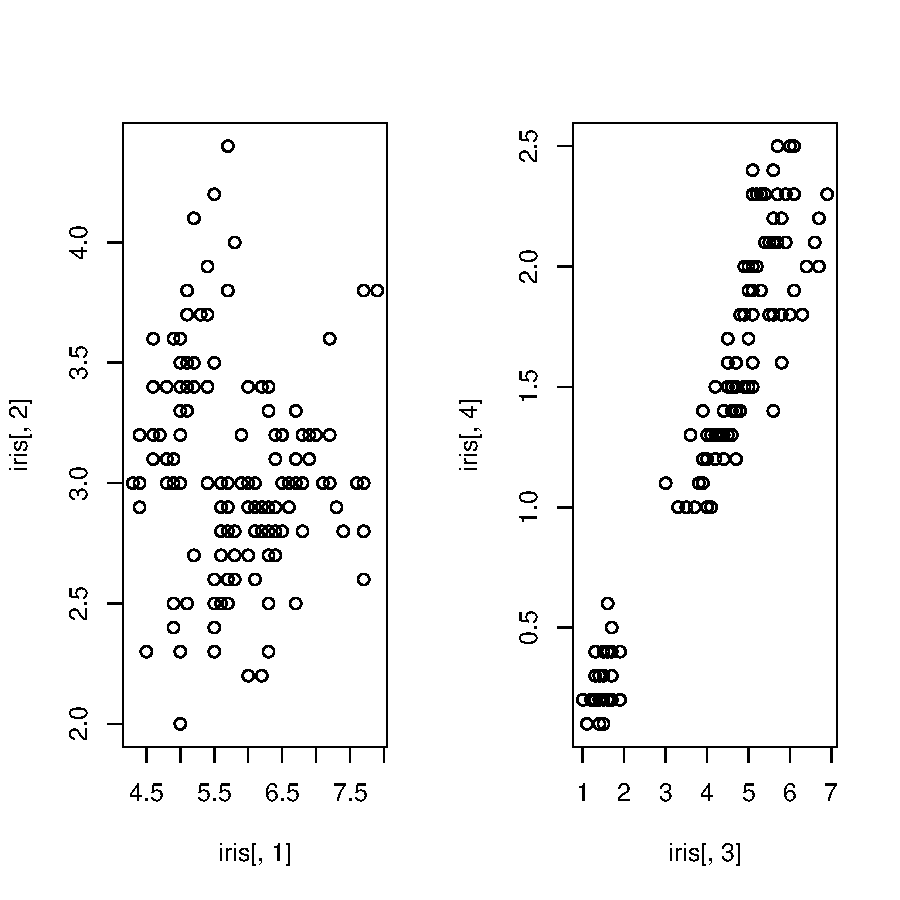
\includegraphics{RbookParte2-218}
\caption{Grafici affiancati con \texttt{mfrow=c(1,2)}}
\label{fig:graficiaffiancati}
\end{center}
\end{figure}

\subsection{Diagrammi a dispersione}
La sintassi di riferimento della funzione \texttt{plot} \index{\texttt{plot}} \`e
\begin{equation*}
\texttt{plot}(\varia{dati},\varia{opzione}_1=val_1, \varia{opzione}_2=val_2,\ldots,\varia{opzione}_n=val_n)\end{equation*}
Scarichiamo da \cite{dasl} il \emph{dataset} che chiameremo \texttt{Gompertz} in cui si studia la mortalit\`a di una popolazione di moscerini al variare dell'et\`a
%code chunk
\begin{Schunk}
\begin{Sinput}
> url="http://lib.stat.cmu.edu/DASL/Datafiles/Medflies.html"
> gompertz<-read.table(url,skip=25,nrow=173,header=T)
\end{Sinput}
\end{Schunk}
\begin{Schunk}
\begin{Sinput}
> class(gompertz)
\end{Sinput}
\begin{Soutput}
[1] "data.frame"
\end{Soutput}
\begin{Sinput}
> head(gompertz)
\end{Sinput}
\begin{Soutput}
  day  living mort.rate
1   0 1203646         0
2   1 1203646    0.0014
3   2 1201913    0.0040
4   3 1197098    0.0051
5   4 1191020    0.0064
6   5 1183419    0.0075
\end{Soutput}
\begin{Sinput}
> par(mfrow=c(1,2))
> plot(gompertz[,1],gompertz[,2])
> plot(gompertz[,1],gompertz[,3])
\end{Sinput}
\end{Schunk}

\begin{figure}\begin{center}
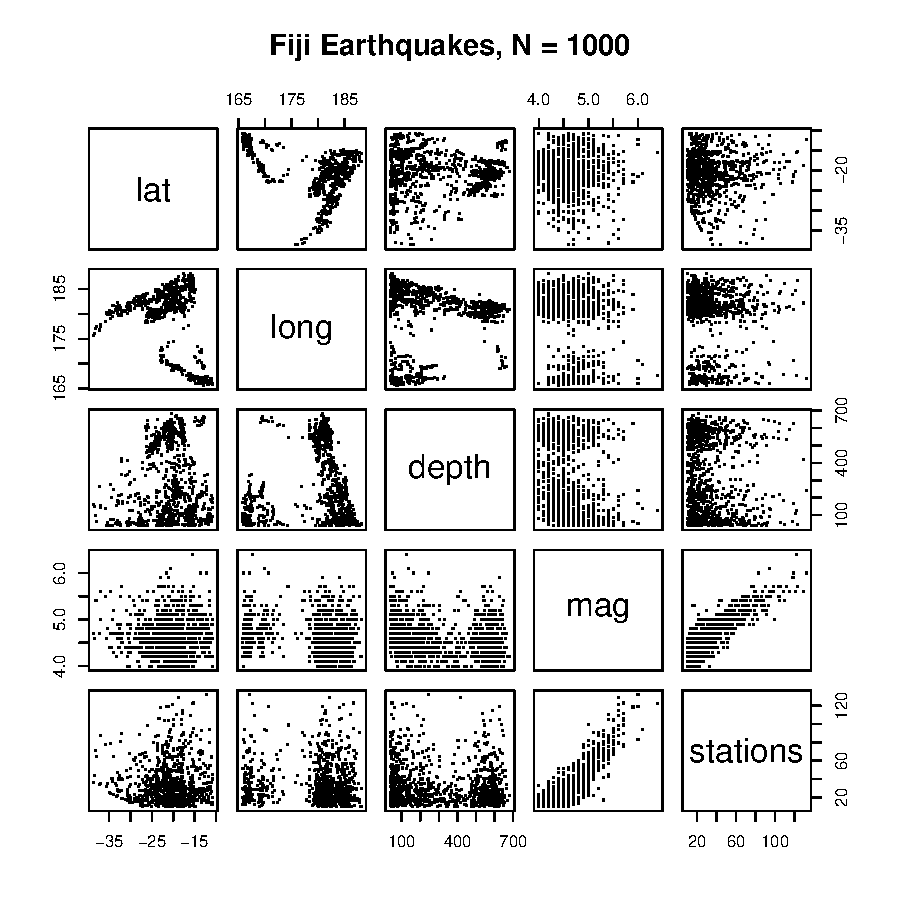
\includegraphics{RbookParte2-222}
\caption{Mortalit\`a dei moscerini. A sinistra la decrescita della popolazione, a destra la mortalit\`a.}
\label{moscerini}
\end{center}
\end{figure}
Il tasso di mortalit\`a (\texttt{mort.rate}) all'istante $t_1$ \`e definito  come rapporto tra numero di individui deceduti nell'intervallo di tempo  $(t_1,t_1+1)$ e  numero di individui all'istante $t_1$. Il comando \texttt{diff} \index{\texttt{diff}} applicato ad una lista ne calcola le differenze termine a termine.
Per esempio
\begin{Schunk}
\begin{Sinput}
> diff(2^(1:10))
\end{Sinput}
\begin{Soutput}
[1]   2   4   8  16  32  64 128 256 512
\end{Soutput}
\end{Schunk}
Il comando che segue consente quindi di verificare la terza colonna di Gompertz
\begin{Schunk}
\begin{Sinput}
> head(-diff(gompertz[,2])/gompertz[-1,2])
\end{Sinput}
\begin{Soutput}
[1] 0.000000000 0.001441868 0.004022227 0.005103189
[5] 0.006422915 0.007592154
\end{Soutput}
\end{Schunk}

Alcune opzioni che possono perfezionare un grafico sono
\begin{itemize}
\item{}\texttt{main}=: assegna il titolo al grafico;
\item{}\texttt{xlab}=: assegna l'etichetta all'asse delle $x$;
\item{}\texttt{ylab}=: assegna l'etichetta all'asse delle $y$;
\item{}\texttt{type}=:
\begin{itemize}
\item{} \texttt{p} Disegna solo i punti.
\item{} \texttt{l} Disegna linee.
\item{} \texttt{b} Disegna entrambi ma senza
sovrapporre le linee ai punti.
\item{} \texttt{o} Disegna linee e punti ma sovrapposti.
\item{} \texttt{n} Non disegna n\'e linee n\'e punti. Serve talora a impostare la finestra grafica.
\end{itemize}
\item{} \texttt{col}=: assegna il colore il cui elenco si ottiene con il comando: \texttt{colors()};
\item{} \texttt{cex}=: un valore numerico, da 0 (sopprime i punti) a valori numerici consigliati minori di 2, definisce la dimensione dei punti;
\item{}\texttt{lty}=: definisce il tipo di linea ({\it line type}), se 1 linea continua, se 2 tratteggiata, se 3 tratteggiata con tratto ridotto, se 4 tratto e punto;
\item{}\texttt{lwd}=: definisce lo spessore della linea ({\it line width}), valori suggeriti tra 0.5 e 2;
\item{} \texttt{pch}=: definisce il \emph{marker} dei punti
\end{itemize}
\footnote{Si noti che tali opzioni coincidono in alcuni casi con opzioni specificabili con \texttt{par}.  In questo caso sono per\`o solo locali. }

Per esempio
\begin{Schunk}
\begin{Sinput}
> par(mfrow=c(2,2))
> gompertz[,c(1,3)]->dati
> plot(dati,main="La mortalit\uE5 dei moscerini", xlab="t (giorni)",
+ ylab="Tasso di mortalit\uE5")
> plot(dati,main="La mortalit\uE5 dei moscerini", xlab="t (giorni)",
+ ylab="Tasso di mortalit\uE5",type="l")
> plot(dati,main="La mortalit\uE5 dei moscerini", xlab="t (giorni)",
+ ylab="Tasso di mortalit\uE5", col="dark green",cex=0.5)
> plot(dati,main="La mortalit\uE5 dei moscerini", xlab="t (giorni)",
+ ylab="Tasso di mortalit\uE5", col="dark green",cex=0.5,
+ lty=4,lwd=2)
\end{Sinput}
\end{Schunk}
Il risultato \`e riportato nella figura~\ref{4moscerini}
\begin{figure}\begin{center}
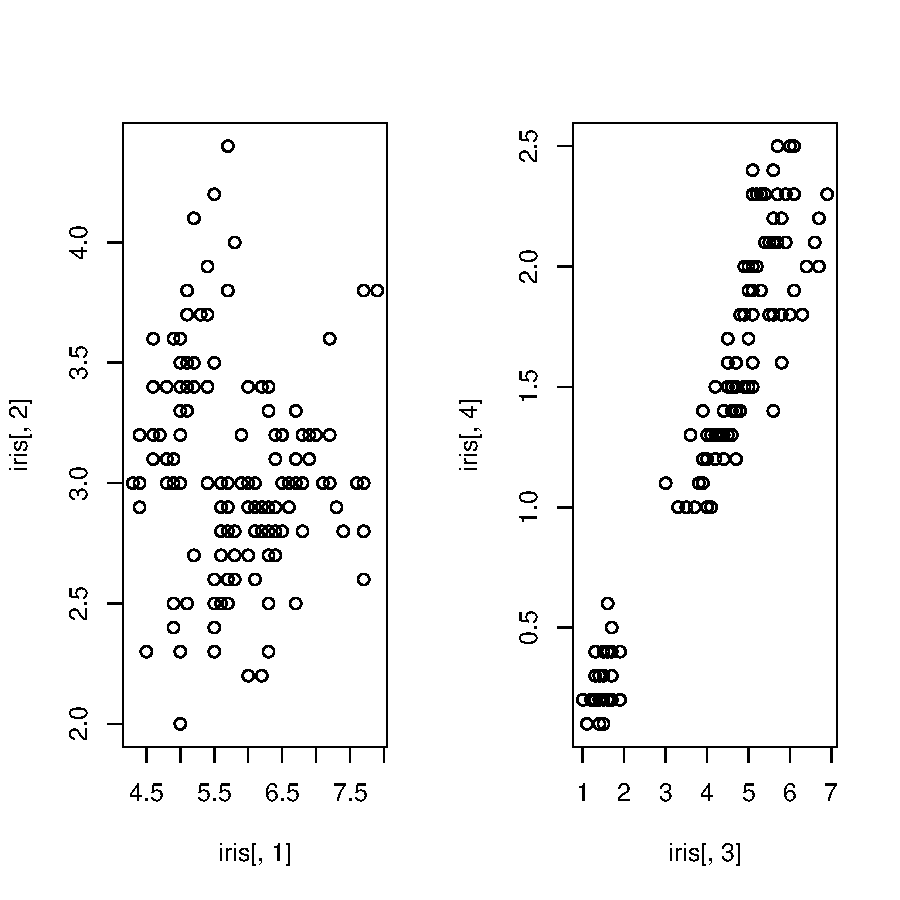
\includegraphics{RbookParte2-226}
\caption{Utilizzo di diversi parametri grafici}
\label{4moscerini}
\end{center}
\end{figure}





\subsection{Grafici multipli e/o sovrapposti}

Analizziamo il {\it dataframe} \texttt{quakes} che riporta numerosi dati sui terremoti che colpiscono la zona delle isole Fiji.
Carichiamo i dati e utilizziamo la funzione \texttt{pairs}\index{pairs} per costruire grafici multipli in un'unica finestra:
\begin{Schunk}
\begin{Sinput}
> quakes
> pairs(quakes, main = "Fiji Earthquakes, N = 1000", cex.main=1.2, pch=".")
\end{Sinput}
\end{Schunk}

\begin{center}
\begin{figure}
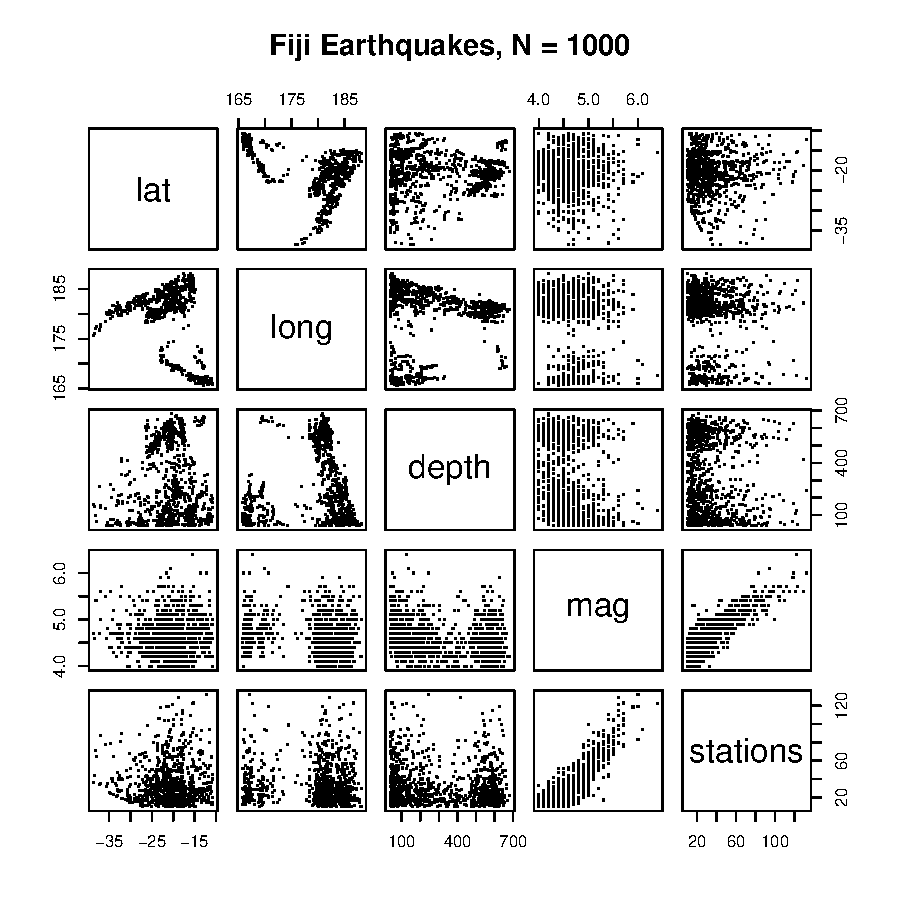
\includegraphics{RbookParte2-228}
\caption{Plot per variabili multiple}
\label{pairplot}
\end{figure}
\end{center}
In effetti il comando \texttt{plot} funziona anche su \emph{dataframe} come \`e verificabile con
\begin{Schunk}
\begin{Sinput}
> methods(plot)
\end{Sinput}
\begin{Soutput}
 [1] plot,ANY-method      plot,Funzione-method
 [3] plot.acf*            plot.correspondence*
 [5] plot.data.frame*     plot.decomposed.ts* 
 [7] plot.default         plot.dendrogram*    
 [9] plot.density*        plot.ecdf           
[11] plot.factor*         plot.formula*       
[13] plot.function        plot.hclust*        
[15] plot.histogram*      plot.HoltWinters*   
[17] plot.isoreg*         plot.lda*           
[19] plot.lm*             plot.mca*           
[21] plot.medpolish*      plot.mlm*           
[23] plot.ppr*            plot.prcomp*        
[25] plot.princomp*       plot.profile*       
[27] plot.profile.nls*    plot.raster*        
[29] plot.ridgelm*        plot.spec*          
[31] plot.stepfun         plot.stl*           
[33] plot.table*          plot.ts             
[35] plot.tskernel*       plot.TukeyHSD*      
see '?methods' for accessing help and source code
\end{Soutput}
\end{Schunk}
e produce lo stesso risultato.
Il grafico risulta complesso da comprendere anche per via delle ridotte dimensioni. Selezioniamo solo i dati relativi alla longitudine ed alla latitudine (prime 2 colonne):
\begin{Schunk}
\begin{Sinput}
>  plot(quakes[,c(1,2)], main = "Fiji Earthquakes, N = 1000", cex.main=1.2, pch=".")
\end{Sinput}
\end{Schunk}
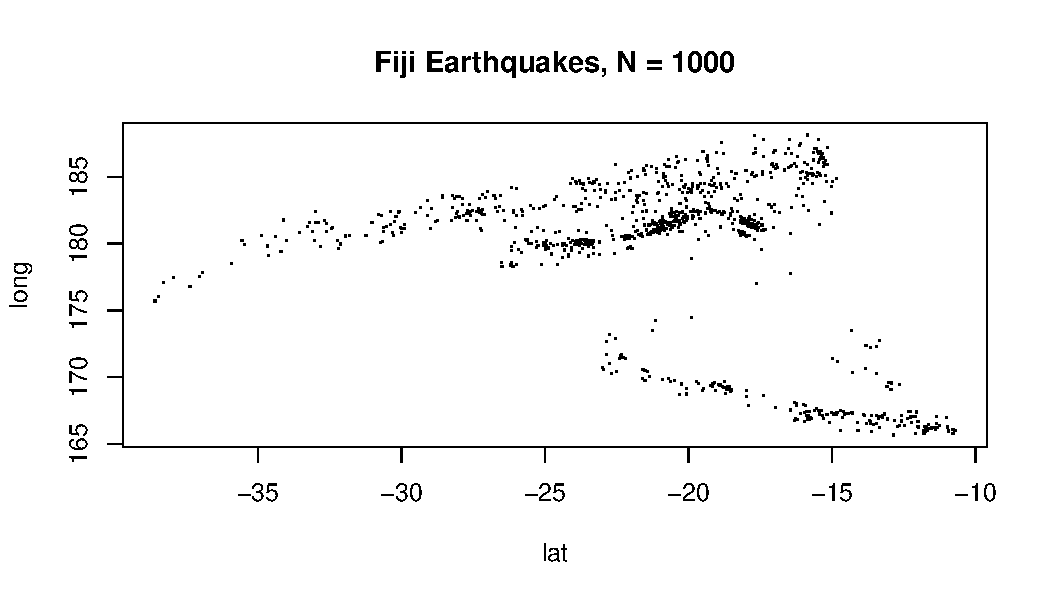
\includegraphics{RbookParte2-230}
\ese{Migliorare questi grafici secondo il gusto personale inserendo, titoli, colorazioni, sfondo, tipo di rappresentazione, tipo di punti, etc.}
\subsection{Aggiungere testo al grafico}
Si pu\`o aggiungere testo in qualunque posizione del grafico, in particolare possiamo posizionare commenti, annotazioni, formule, ecc. Si devono solo specificare coordinate e testo, oltre ad altri parametri visualizzabili con \texttt{?text}.
Nell'esempio seguente generiamo i vertici di un poligono regolare con numero di lati uguali al numero di lettere dell'alfabeto.
\begin{Schunk}
\begin{Sinput}
> set.seed(20)#inizializza il generatore
> nl=length(letters)#numero di lettere
> coord.poli=matrix(c(cos(2* pi *(1:nl)/nl), sin (2*pi*(1:nl)/nl)),
+ nc=2,nrow=nl);#vertici del poligono
> coord.random<-matrix(runif(2*nl),nc=2,nrow=nl)#perturbazione
> coord=coord.random+3*coord.poli;#coordinate perturbate
> #plot(coord,col="blue",lwd=4,lty=1,type="l")
> #text(coord,letters,col="red",cex=1.6,adj=2)#inserimento del testo
> plot(coord,col="blue",lwd=4,lty=1,type="n")
> polygon(coord,col="yellow",density=10,angle=30)
> text(coord,letters,col="red")
\end{Sinput}
\end{Schunk}
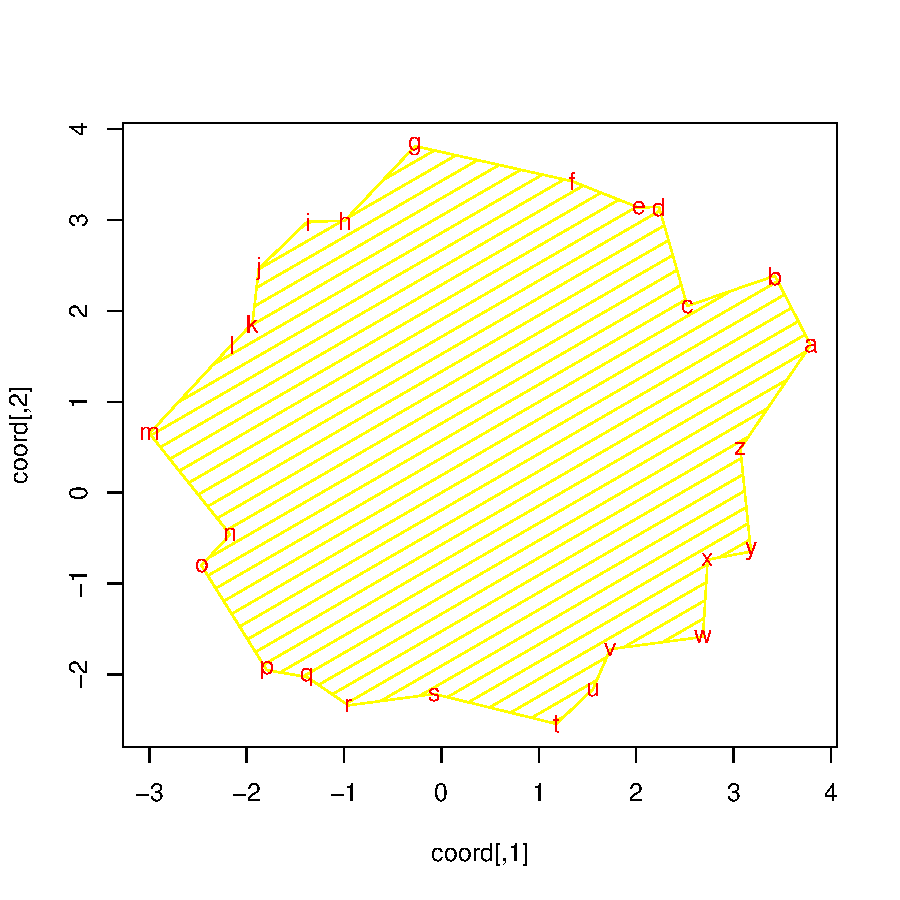
\includegraphics{RbookParte2-231}

Il parametro  \texttt{adj} sposta il testo rispetto alle coordinate
\subsection{Immagini di un vulcano}
Vediamo alcune rappresentazioni grafiche 3D.
\begin{Schunk}
\begin{Sinput}
> #require(grDevices);
> #require(graphics)
> filled.contour(volcano, color.palette = terrain.colors, asp = 1)
> title(main = "volcano data: filled contour map")
\end{Sinput}
\end{Schunk}
\begin{figure}[htbp]
\begin{center}

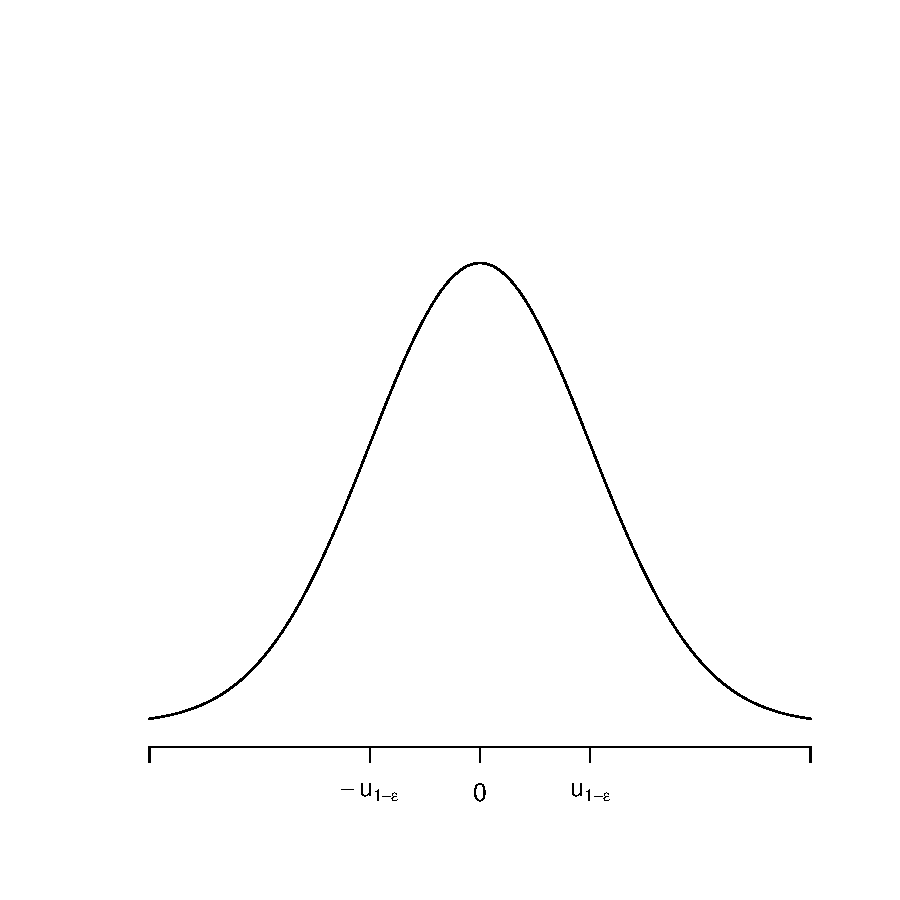
\includegraphics{RbookParte2-233}
\caption{Linee di livello}
\label{vulcano1}
\end{center}
\end{figure}


\begin{Schunk}
\begin{Sinput}
> x<- c(0.00, 0.40, 0.86, 0.85, 0.69, 0.48, 0.54, 1.09, 1.11, 1.73, 2.05, 2.02)
> par(bg="lightgray")
> plot(x, type="n", axes=FALSE, ann=FALSE)
> usr <- par("usr")
> rect(usr[1], usr[3], usr[2], usr[4], col="cornsilk", border="black")
> lines(x, col="blue")
> points(x, pch=21, bg="lightcyan", cex=1.25)
> axis(2, col.axis="blue", las=1)
> axis(1, at=1:12, lab=month.abb, col.axis="blue")
> box()
> title(main="Interesse per R", font.main=4, col.main="red")
> title(xlab="1996", col.lab="red")
\end{Sinput}
\end{Schunk}
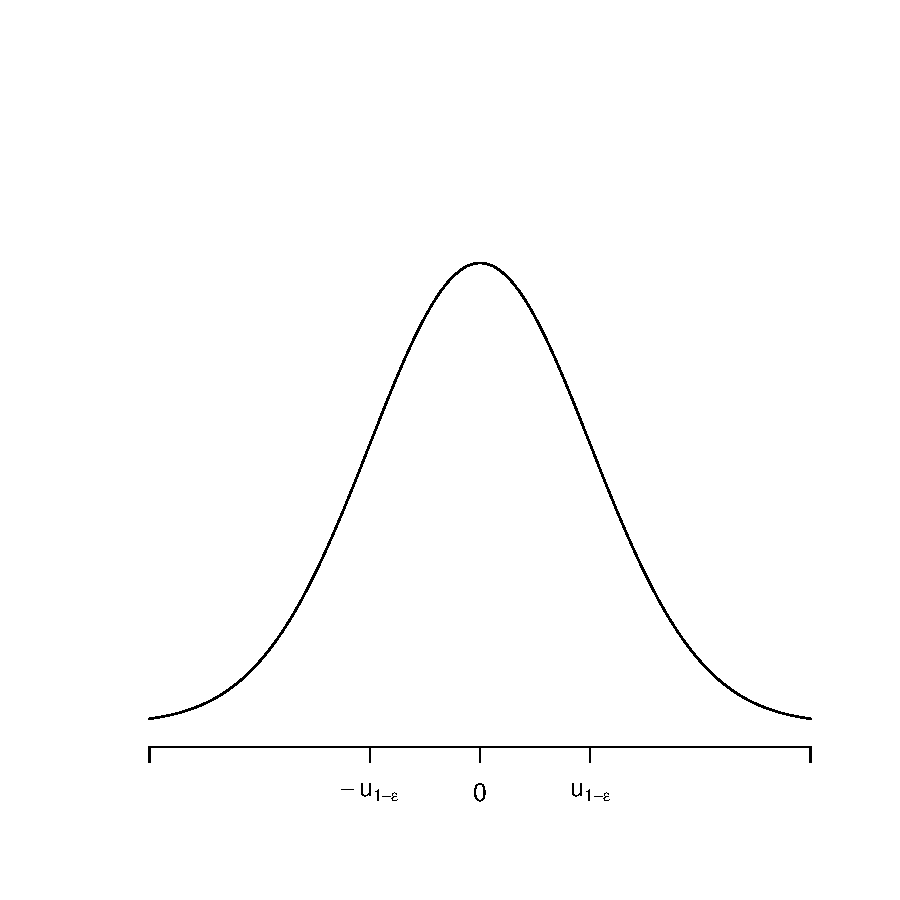
\includegraphics{RbookParte2-234}

Un esempio:
\begin{Schunk}
\begin{Sinput}
> boxplot(len~dose, data = ToothGrowth,
+ boxwex = 0.25, at = 1:3 - 0.2,
+ subset = supp == "VC", col = "yellow",
+ main = "Guinea Pigs' Tooth Growth",
+ xlab = "Vitamin C dose mg",
+ ylab = "tooth length")
\end{Sinput}
\end{Schunk}
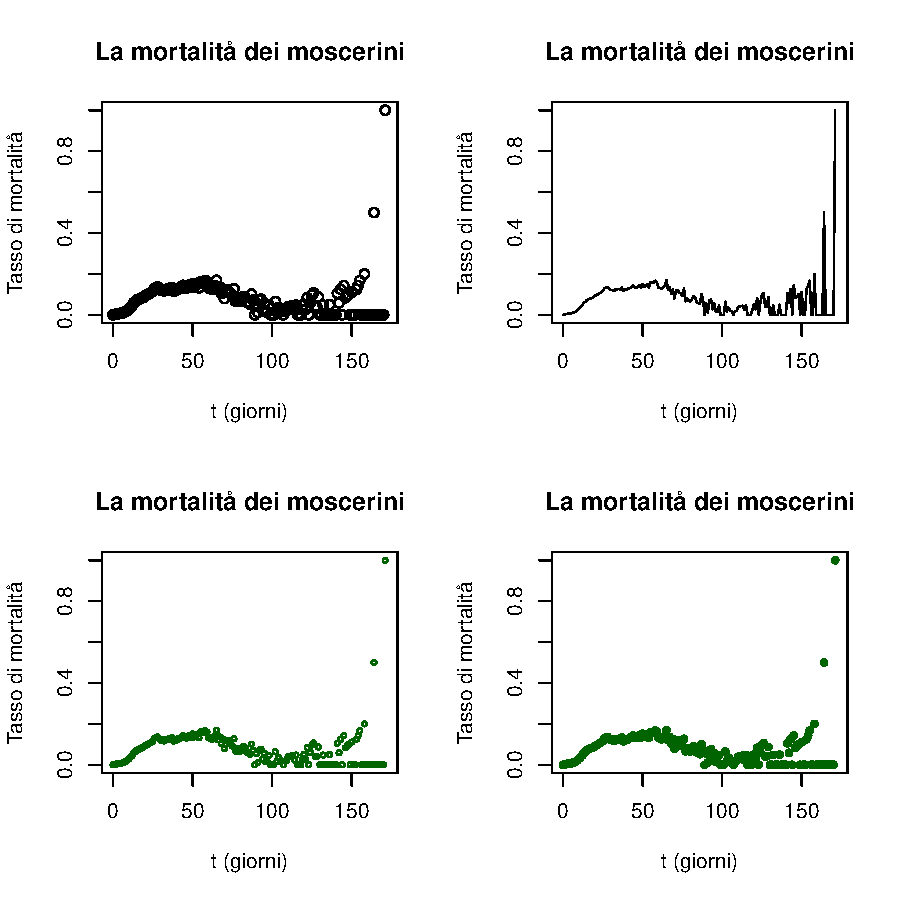
\includegraphics{RbookParte2-236}

\subsection{I rettangoli }
\textsf{R} consente di disegnare forme (dette primitive) come rettangoli o poligoni. I rettangoli in particolare sono molto utili e versatili, consentendo di realizzare riquadri, evidenziare regioni grafiche, ecc.
%code chunk
\begin{Schunk}
\begin{Sinput}
> plot(c(100, 200), c(300, 450), type= "n", xlab="", ylab="")
> rect(100, 300, 125, 350) # transparent
> rect(100, 400, 125, 450, col="green", border="blue") # coloured
> rect(115, 375, 150, 425, col=par("bg"), border="transparent")
> rect(150, 300, 175, 350, density=10, border="red")
> rect(150, 400, 175, 450, density=30, col="blue", angle=-30, border="transparent")
> legend(180, 450, legend=1:4, fill=c(NA, "green", par("fg"), "blue"),
+ density=c(NA, NA, 10, 30), angle=c(NA, NA, 30, -30))
\end{Sinput}
\end{Schunk}
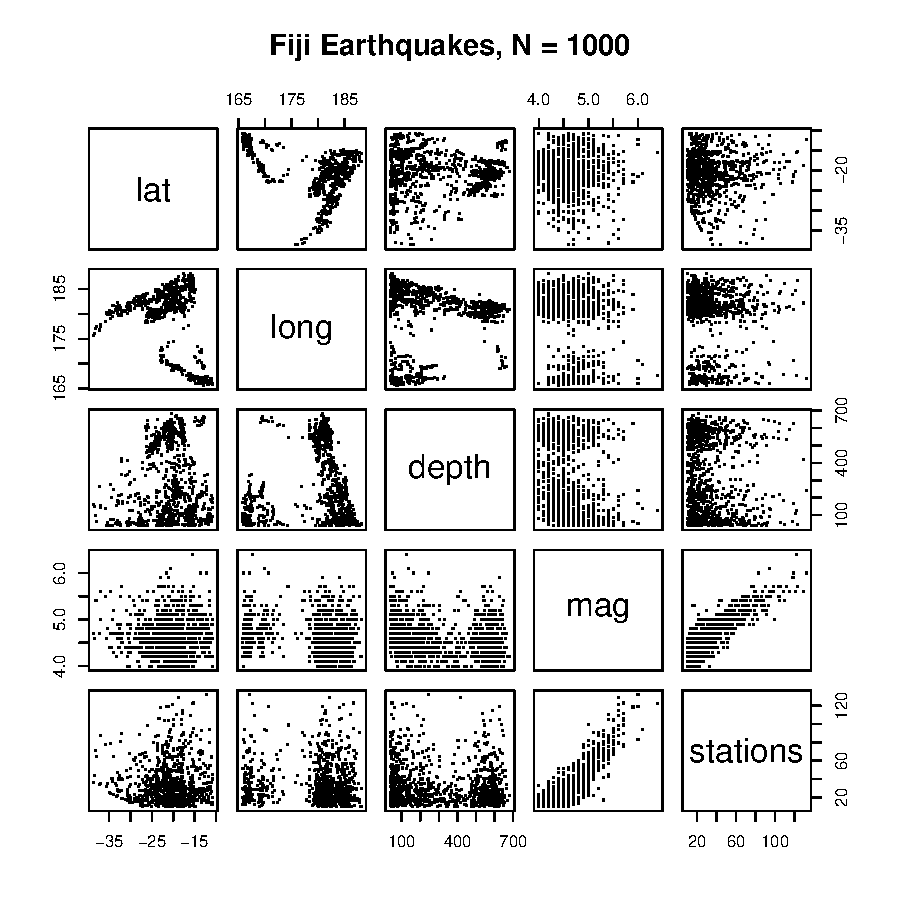
\includegraphics{RbookParte2-237}

\section{Grafici professionali: legenda, annotazioni e formule}
Ricordiamo che una volta che sia  assegnato il livello di fiducia $1-\epsilon$, il numero $u_{1-\epsilon}$ che leggiamo nelle tabelle  distribuzione normale \`e il valore dell'ascissa tale che nell'intervallo $[-u_{1-\epsilon},u_{1-\epsilon}]$  cada un'area pari al livello di fiducia; in altre parole le 2 code della distribuzione vengono rimosse.
Vogliamo ora creare un grafico illustrativo di questa definizione.

Tracceremo inizialmente un grafico della normale tra $[-3,3]$ scegliendo come valore dell'ascissa
$u_{1-\epsilon}$  il numero  1.  Vogliamo quindi scrivere l'espressione $u_{1-\epsilon}$ nel punto di ascissa  1 e il suo opposto nel punto di ascissa -1 dell'asse $x$.
Per disegnare delle tacche sugli assi e assegnare valori alfanumerici alle stesse
si pu\`o utilizzare Il comando\selectlanguage{english}
\begin{eqnarray*}
\texttt{axis}(\varia{num},\texttt{c}(\varia{tacca}_1,\varia{tacca}_2,\ldots,\varia{tacca}_\varia{n}),\\
\texttt{c("}\varia{nome}_1, \texttt{"}\varia{nome}_2 \texttt{"},\ldots,\texttt{"}\varia{nome}_\varia{n}\texttt{"}))
\end{eqnarray*}
\selectlanguage{italian}
Qui $\varia{tacca}$ rappresenta il valore della coordinata mentre $\varia{num}$ \`e un indice che rappresenta  l'asse in esame  come segue 1=sotto, 2=sinistra, 3=sopra and 4=destra.

Possiamo  procedere con
\begin{Schunk}
\begin{Sinput}
> curve(dnorm(x),-3,3,axes=FALSE,ylab="",xlab="",ylim=c(0,0.5))
> axis(1,c(-3,-1,0,1,3),c("",expression(-u[1-epsilon]),0,expression(u[1-epsilon]),""))
\end{Sinput}
\end{Schunk}

\begin{figure}\begin{center}
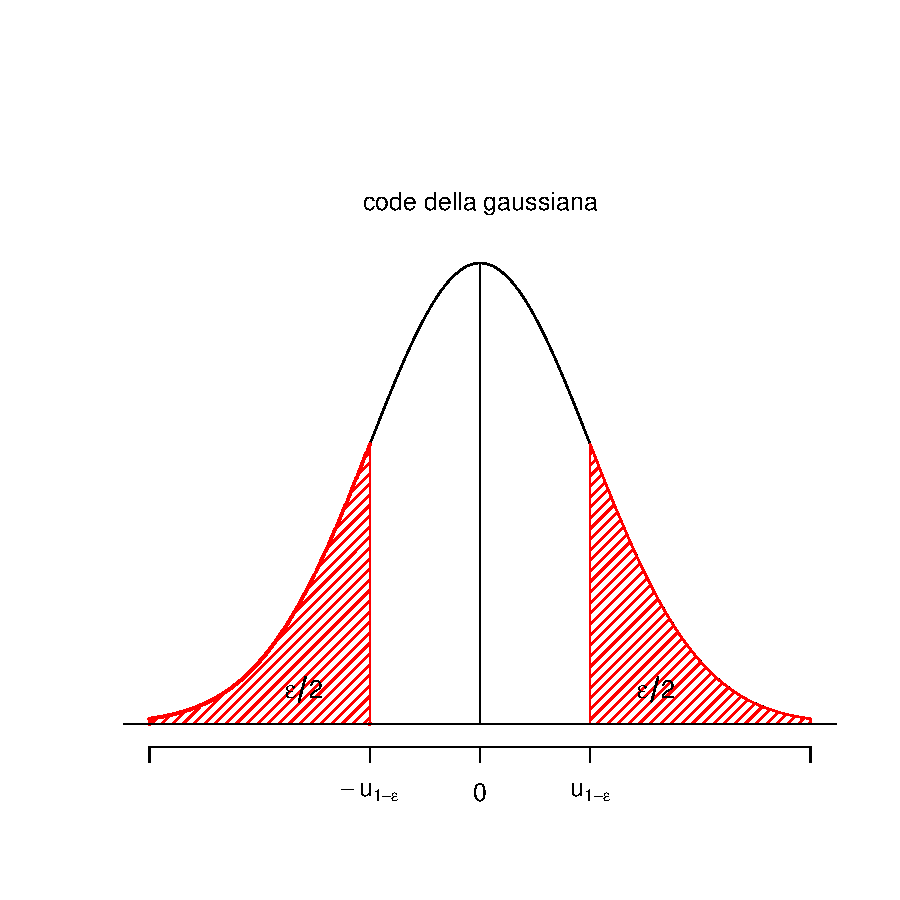
\includegraphics{RbookParte2-239}
\caption{Selezione delle etichette sull'asse $x$. }
\label{normale13}
\end{center}
\end{figure}

Il comando \texttt{expression} consente di scrivere simboli e anche lettere greche.
Come uscita di questo primo comando troviamo il grafico~(\ref{normale13})
Per evidenziare le 2 code tratteggiamo l'area sottesa dalla normale tra 1 e 3  (e in seguito da  -3 a -1). Per operare questo tratteggio si approssima
la regione da tratteggiare con un poligono con un numero molto elevato (200) di vertici definiti come segue
%code chunk
\begin{Schunk}
\begin{Sinput}
> xmin<-1;xmax<-3;
> npunti<-200
> f=dnorm#selezione degli  estremi
> #e del numero di punti base del poligono
> vals<-seq(xmin,xmax,length=npunti)
> x<-c(xmin,vals,xmax,xmin)
> y<-c(0,f(vals),0,0);
\end{Sinput}
\end{Schunk}

La sintassi di \texttt{polygon}?\`e
\begin{eqnarray*}
\texttt{polygon}(\varia{x,y},\texttt{density}=\varia{val1},
\texttt{angle}=\varia{val2},
\\
\texttt{col=\virgolette col\virgolette
})
\end{eqnarray*}

Il comando
\begin{Schunk}
\begin{Sinput}
> curve(dnorm(x),-3,3,axes=FALSE,ylab="",xlab="",ylim=c(0,0.5))
> axis(1,c(-3,-1,0,1,3),c("",expression(-u[1-epsilon]),0,expression(u[1-epsilon]),""))
> points(x,y,pch=20,col="red",cex=0.2)
\end{Sinput}
\end{Schunk}
consente la visualizzazione dei punti ottenuti (come in figura~(\ref{normale200punti})).

\begin{figure}\begin{center}
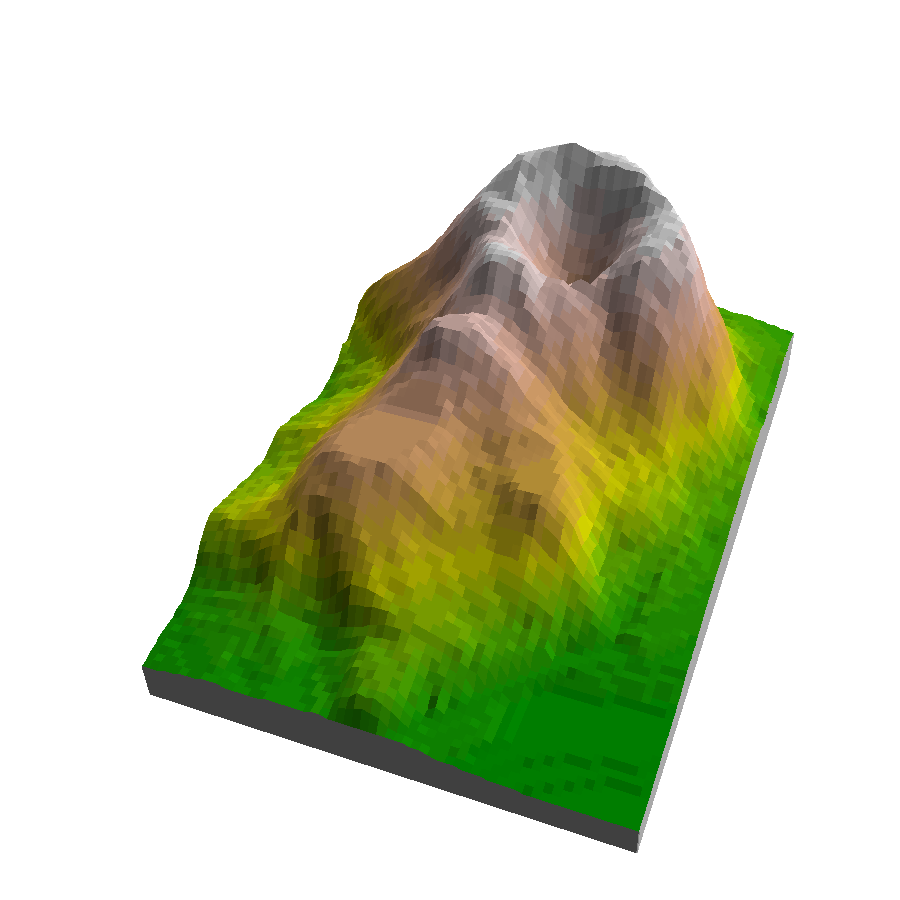
\includegraphics{RbookParte2-242}
\caption{ Selezione dei punti per l'ombreggiamento di una regione poligonale}
\label{normale200punti}
\end{center}
\end{figure}

Questi punti  possono poi essere uniti con una curva poligonale
\begin{Schunk}
\begin{Sinput}
> curve(dnorm(x),-3,3,axes=FALSE,ylab="",xlab="",ylim=c(0,0.5))
> axis(1,c(-3,-1,0,1,3),c("",expression(-u[1-epsilon]),0,expression(u[1-epsilon]),""))
> points(x,y,pch=20,col="red",cex=0.2)
> polygon(x,y,density=20,angle=45,col="RED")
> x<--x
> y<-c(0,dnorm(-vals),0,0)
> polygon(x,y,density=20,angle=45,col="RED")
\end{Sinput}
\end{Schunk}

Infine possiamo riportare i valori delle aree delle 2 code, evidenziare l'asse di simmetria  e dare un titolo al grafico


\begin{Schunk}
\begin{Sinput}
> curve(dnorm(x),-3,3,axes=FALSE,ylab="",xlab="",ylim=c(0,0.5))
> axis(1,c(-3,-1,0,1,3),c("",expression(-u[1-epsilon]),0,expression(u[1-epsilon]),""))
> points(x,y,pch=20,col="red",cex=0.2)
> polygon(x,y,density=20,angle=45,col="RED")
> x<--x
> y<-c(0,dnorm(-vals),0,0)
> polygon(x,y,density=20,angle=45,col="RED")
> polygon(x,y,density=20,angle=45,col="RED")
> abline(h=min(y))
> text(0,0.45,expression("code della gaussiana"))
> text(-1.6,0.03,expression(epsilon/2))
> text(1.6,0.03,expression(epsilon/2))
> lines(c(0,0),c(0,dnorm(0)))
\end{Sinput}
\end{Schunk}
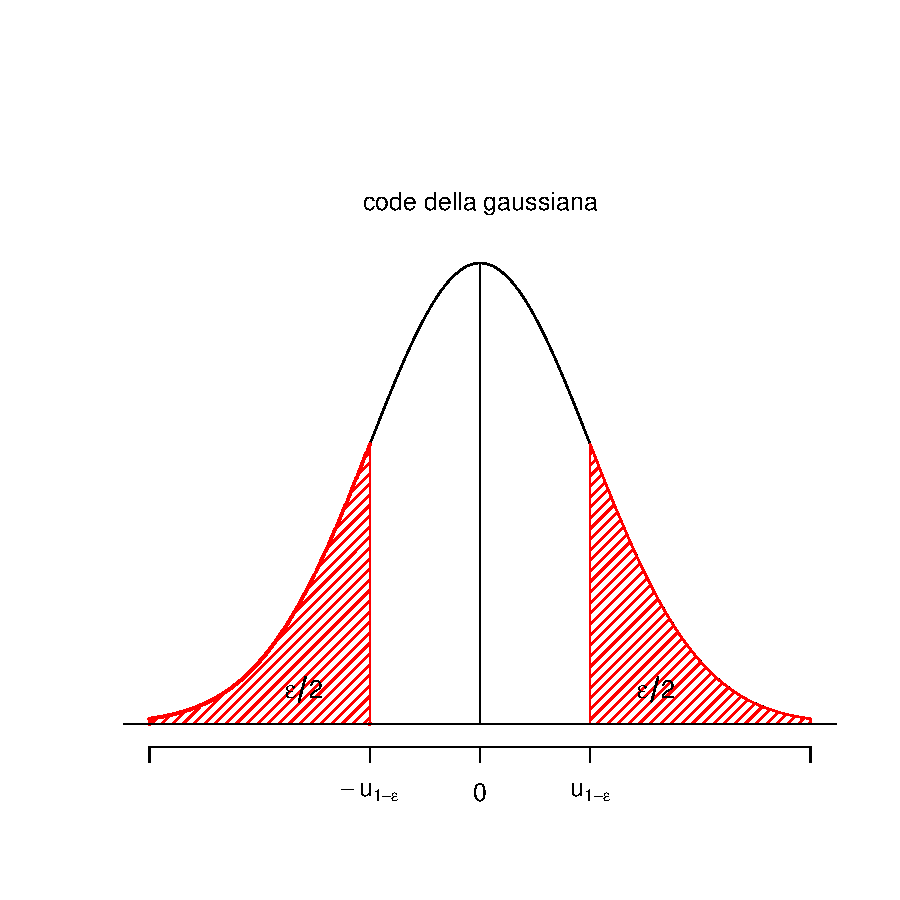
\includegraphics{RbookParte2-244}

\begin{figure}\begin{center}
\begin{Schunk}
\begin{Sinput}
> curve(dnorm(x),-3,3,axes=FALSE,ylab="",xlab="",ylim=c(0,0.5))
> polygon(x,y,density=20,angle=45,col="RED")
> abline(h=min(y))
> text(0,0.45,expression("code della gaussiana"))
> text(-1.6,0.03,expression(epsilon/2))
> text(1.6,0.03,expression(epsilon/2))
> lines(c(0,0),c(0,dnorm(0)))
\end{Sinput}
\end{Schunk}
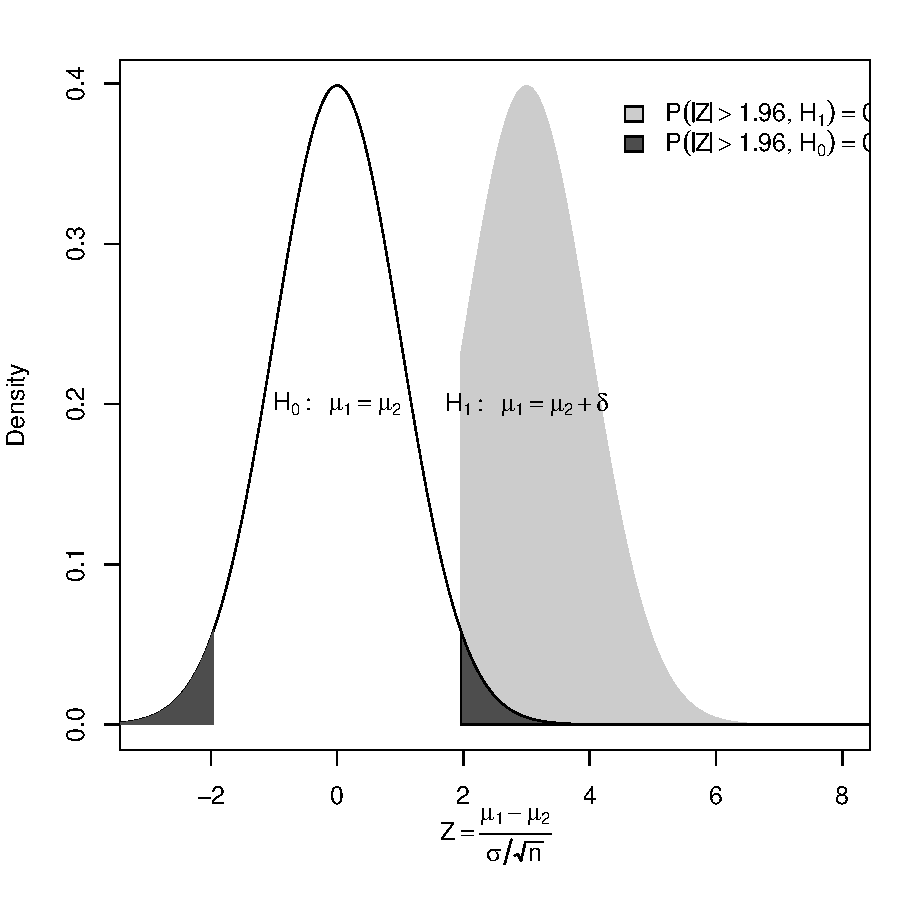
\includegraphics{RbookParte2-245}
\caption{ Area delle code della distribuzione normale. Il valore di $u_{1-\epsilon}$ \`e quello riportato nella  tabella della distribuzione normale. }
\label{normaletratto}
\end{center}
\end{figure}

\section{Pittura virtuale}
Iniziamo a disegnare dei rettangoli, di coordinate casuali ma entro un dato range, di colore casuale, con spessore del bordo casuale.
\begin{Schunk}
\begin{Sinput}
> par(bg="skyblue");
> plot(0,xlim=c(0.3,1),ylim=c(0.3,1),axes=F, xlab="",ylab="")
> for(i in 1:100)
+ { Sys.sleep(0.01);
+ runif(1)->sotto;
+ runif(1)->sinistra;
+ runif(1)+sotto->sopra;
+ runif(1)+sinistra->destra;
+ bordi<-0;for(i in 1:100) bordi[i]<-floor(runif(1,1,10))
+ spess<-0;for(i in 1:100) spess[i]<-floor(runif(1,1,10))
+ rect(sinistra,sotto,destra,sopra,col=rgb(runif(1),runif(1),runif(1)),border=bordi[i],lwd=spess)}
\end{Sinput}
\end{Schunk}
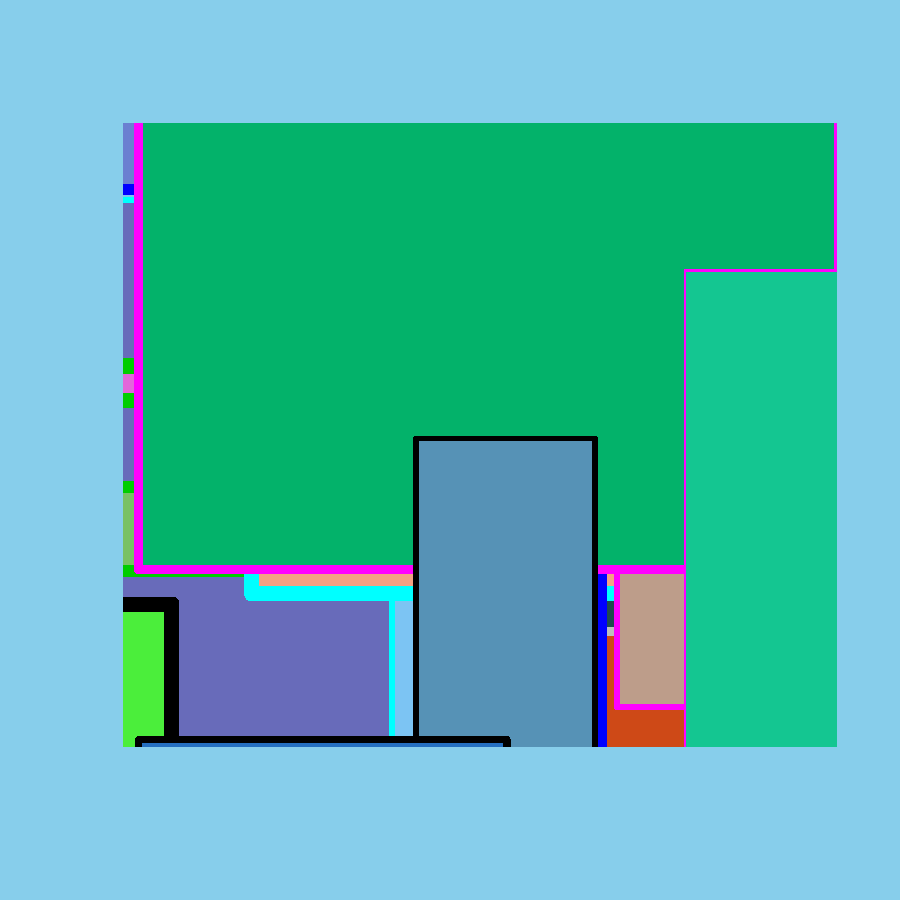
\includegraphics{RbookParte2-246}
\section{Grafica 3D, il vulcano Maunga Whau}
Con il codice che segue

\begin{Schunk}
\begin{Sinput}
> z<- 2 * volcano
> x<- 10 * (1:nrow(z))
> y<- 10 * (1:ncol(z))
> z0<- min(z) - 20
> z<- rbind(z0, cbind(z0, z, z0), z0)
> x<- c(min(x) - 1e-10, x, max(x) + 1e-10)
> y<- c(min(y) - 1e-10, y, max(y) + 1e-10)
> fill <- matrix("green3", nr = nrow(z)-1, nc = ncol(z)-1)
> fill[ , i2 <- c(1,ncol(fill))] <- "gray"
> fill[i1 <- c(1,nrow(fill)) , ] <- "gray"
> fcol <- fill
> zi <- volcano[ -1,-1] + volcano[ -1,-61] +
+ volcano[-87,-1] + volcano[-87,-61] ## / 4
> fcol[-i1,-i2] <- terrain.colors(20)[cut(zi, quantile(zi, seq(0,1, len = 21)),
+ include.lowest = TRUE)]
> par(mar=rep(.5,4))
> persp(x, y, 2*z, theta = 110, phi = 40, col = fcol, scale = FALSE,
+ ltheta = -120, shade = 0.4, border = NA, box = FALSE)
\end{Sinput}
\end{Schunk}
otteniamo la figura~\ref{vulcano3D}. Il comando di base \`e \texttt{persp} che richiede una griglia di valori di $(x,y)$ e il corrispondente valore di quota.
\begin{figure}[htbp]
\begin{center}
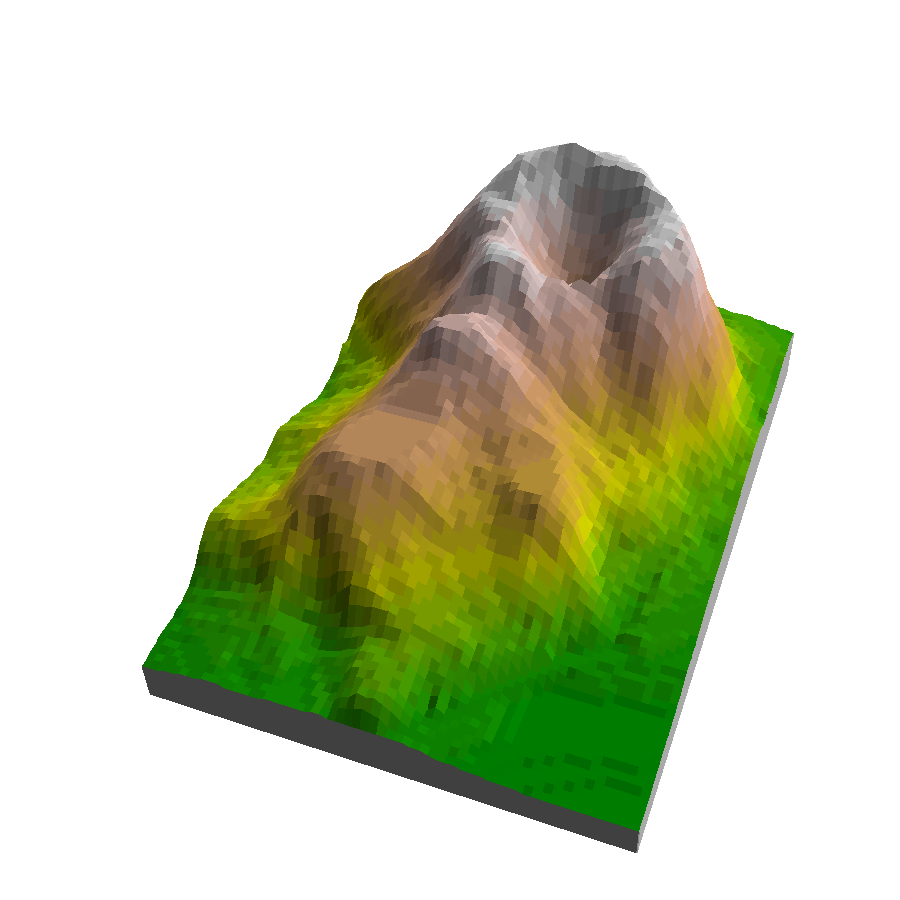
\includegraphics{RbookParte2-248}

\caption{Grafica 3 dimensionale, ottenuta con il comando \texttt{persp}}
\label{vulcano3D}
\end{center}
\end{figure}

 Costruiamo due curve che rappresentano due distribuzioni normali, in particolare al posto della funzione \texttt{dnorm} andremo a calcolare i singoli valori di $y$ associati ad un set di valori di
$x$, essendo poi liberi di utilizzare la funzione \texttt{plot}


\begin{Schunk}
\begin{Sinput}
> options(width=60)
> x<-seq(-10,10,length=400)
> y1<-dnorm(x)
> y2<-dnorm(x,m=3)
> par(mar=c(5,4,2,1))
> plot(x, y2, xlim=c(-3,8), type="n", xlab=quote(Z==frac(mu[1]-mu[2],
+ sigma/sqrt(n))), ylab="Density")
> polygon(c(1.96,1.96,x[240:400],10), c(0,dnorm(1.96,m=3),y2[240:400],0),
+ col="grey80", lty=0)
> lines(x, y1)
> polygon(c(-1.96,-1.96,x[161:1],-10), c(0,dnorm(-1.96,m=0), y1[161:1],0),
+ col="grey30", lty=0)
> polygon(c(1.96, 1.96, x[240:400], 10), c(0,dnorm(1.96,m=0),
+ y1[240:400],0), col="grey30")
> legend(4.2, .4, fill=c("grey80","grey30"),
+ legend=expression(P(abs(Z)>1.96, H[1])==0.85,
+ P(abs(Z)>1.96,H[0])==0.05), bty="n")
> text(0, .2, quote(H[0]:~~mu[1]==mu[2]))
> text(3, .2, quote(H[1]:~~mu[1]==mu[2]+delta))
\end{Sinput}
\end{Schunk}
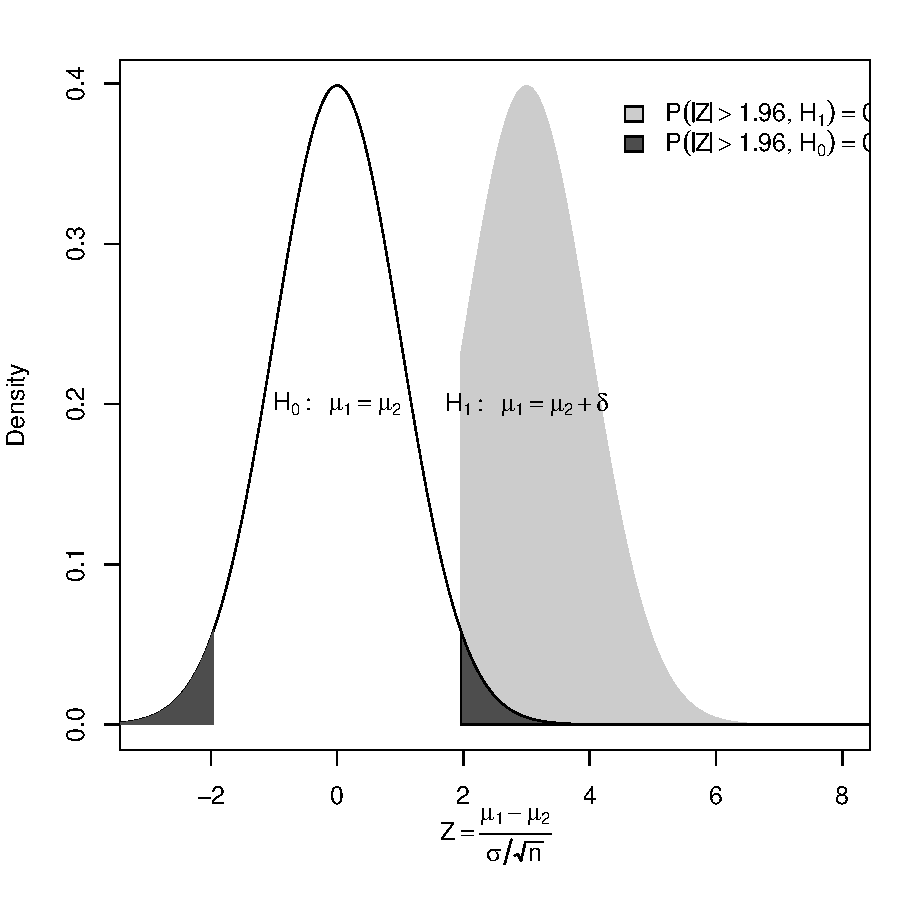
\includegraphics{RbookParte2-249}


\section{Web}
In questa sezione vedremo come collegarsi al \emph{web}, come leggere il contenuto di file \texttt{.html}, come aprire indirizzi web nel browser.
La funzione \texttt{readLines} consente di leggere il codice sorgente \texttt{(.html)} di un determinato sito web. Il numero che segue l'indirizzo definisce il numero di righe che si vogliono leggere.
Se invece vogliamo aprire una pagina web direttamente nel browser utilizziamo \texttt{browseURL},\index{browseURL}
definendo il browser (il default \`e dipendente dalle preferenze dell'utente e soprattutto dal sistema operativo).

\begin{Schunk}
\begin{Sinput}
> readLines("http://www.r-project.org/",4)
\end{Sinput}
\end{Schunk}
%http://www.youtube.com/watch?v=ZwYQPtU2Pa0
\begin{Schunk}
\begin{Sinput}
> channel="http://www.youtube.com/watch?v=W2GZFeYGU3s&feature=related"
\end{Sinput}
\end{Schunk}
\begin{Schunk}
\begin{Sinput}
> browseURL(channel,browser=getOption("browser"))
\end{Sinput}
\end{Schunk}

\subsection{Colori}

\subsection{Costruire una funzione per realizzare grafica su {\it device}}
Lo scopo di questa procedura \`e quello di  realizzare una funzione, che chiameremo \texttt{mondrian}, che ci consentir\`a di contenere ed eseguire il codice necessario per disegnare la riproduzione  del quadro che alcuni di voi hanno manualmente digitato la scorsa lezione. Gli step necessari
per realizzare ci\`o sono i seguenti:
\begin{itemize}
\item{1.} Copiare in locale il codice per realizzare la figura su \emph{device};
\item{2.} Inserire questo codice nella funzione mondrian, che realizziamo con il comando fix(mondrian);
\item{3.} Richiamare la funzione con il comando: mondrian()
\item{4.} Verificare che sia stato prodotto il file mondrian.png e sua apertura. Se non specifichiamo l'indirizzo del file esso si trover\`a nella cartella di lavoro di \textsf{R}, ottenibile con il comando getwd().
\end{itemize}
\section{Grafica 3D, grafico di una funzione di due variabili}
La funzione di base in \textsf{R} per realizzare grafica 3D statica \`e \texttt{persp}.
Gli input richiesti sono due vettori (coordinate sulle $x$ e sulle $y$) ed una matrice (di ingressi ingressi $x$ e $y$, contenente
all'incrocio $z$).


\begin{Schunk}
\begin{Sinput}
> f<-function(x,y)  y^2+ x^2
> xset<-seq(-1,1,length=101)
> yset<-seq(-1,1,length=101)
> zmatr<-matrix(0,length(xset),length(yset))
> for(i in 1:length(xset)) for(j in 1:length(yset)) zmatr[i,j]<-f(xset[i],xset[j]);
> persp(xset,yset,zmatr)##persp possiede parametri di rotazione, colorazione, ombreggiatura, ecc.
> persp(xset,yset,zmatr,theta = 30, phi = 60, r = 10, d = 10)
\end{Sinput}
\end{Schunk}


\subsection{Il pacchetto \texttt{rgl}}

Il pacchetto \texttt{rgl} si compone di funzioni per la grafica 3D dinamica e consente di realizzare grafici ruotabili, eventualmente animati e sicuramente di grande impatto e potenzialit\`a.
Il comando base per aprire una \emph{device} grafica di \texttt{rgl} \`e \texttt{open3d()}.
Cominciamo con il disegnare un solido, in particolare un cubo, mediante il comando \texttt{shade3d},
Prestiamo attenzione alla  generazione della lista dei   colori (\texttt  {rep} \`e un comando molto potente):

\begin{Schunk}
\begin{Sinput}
> library(rgl)
> rgl.postscript(file="cubo.eps")
> shade3d(cube3d(color=rep(rainbow(6),rep(4,6))))
\end{Sinput}
\end{Schunk}
\begin{figure}[htbp]
\begin{center}
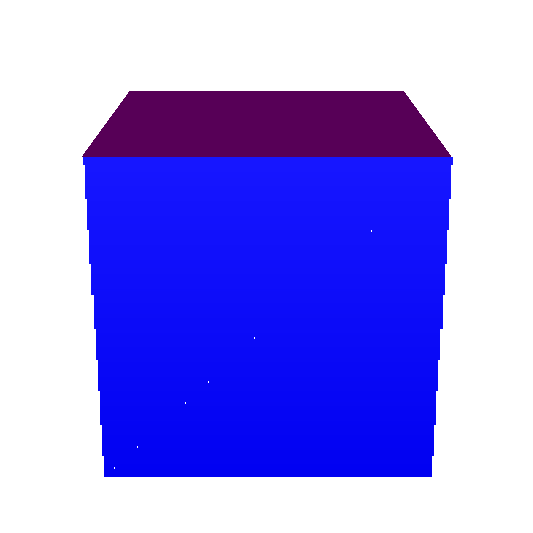
\includegraphics[height=2.in]{../grafici/cubo.pdf}
\caption{{\bf default}}
\label{default}
\end{center}
\end{figure}

II comando \texttt{plot3d} \`e  il pi\`u semplice ed immediato comando per realizzare un grafico tridimensionale. Esso richiede come input le coordinate $(x,y,z)$ dei punti da rappresentare.
Nell'esempio generiamo 1000 punti, notate la colorazione ed il grafico rotabile (mentre con il tasto destro del mouse si esegue lo zoom).
%code chunk
\begin{Schunk}
\begin{Sinput}
> rgl.postscript(file="1000punti.eps")
> open3d()
> x <- sort(rnorm(1000))
> y <- rnorm(1000)
> z <- rnorm(1000)
> plot3d(x, y, z, col=rainbow(1000), size=2)
> dev.off()
\end{Sinput}
\end{Schunk}
otteniamo cos? la figura
\begin{figure}[htbp]
\begin{center}
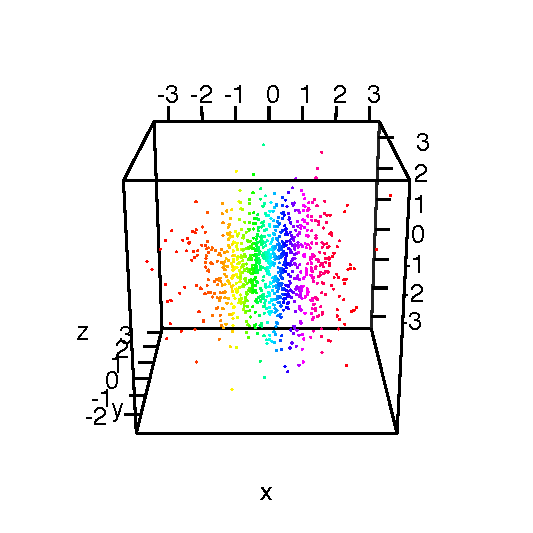
\includegraphics[scale=0.8]{../grafici/1000punti.pdf}
\caption{Risultato \texttt{plot3D}}
\label{defaue}
\end{center}
\end{figure}

Ora riprendiamo le coordinate del Maunga Whau e rappresentiamolo con il comando \index{\texttt{surface3d}}, il quale possiede numerosi parametri di ombreggiatura, tonalit\`a e sfumature di colorazioni, tutte ottenibili dal comando \texttt{par3d}\index{\texttt{par3D}}. Il vulcano:
\begin{Schunk}
\begin{Sinput}
> library(rgl)
> rgl.postscript(file="../grafici/vulcano.eps")
> data(volcano)
> z <- 2 * volcano
> x <- 10 * (1:nrow(z))
> y <- 10 * (1:ncol(z))
> zlim <- range(y)
> zlen <- zlim[2] - zlim[1] + 1
> colorlut <- terrain.colors(zlen)
> col <- colorlut[ z-zlim[1]+1 ]
> open3d()
> surface3d(x, y, z, color=col, back="lines")
\end{Sinput}
\end{Schunk}

\begin{figure}[htbp]
\begin{center}
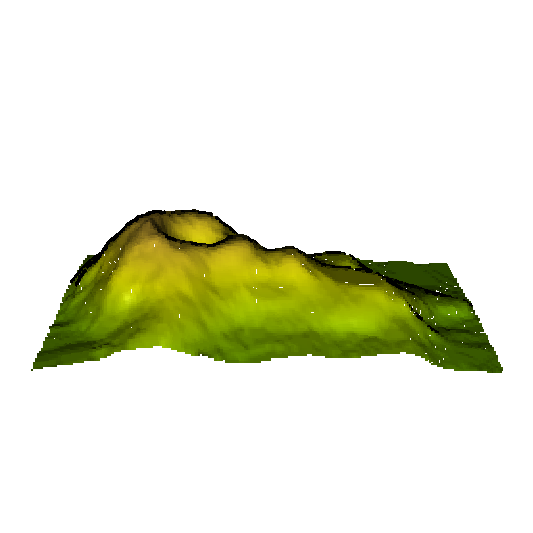
\includegraphics[scale=0.8]{../grafici/vulcano.pdf}
\caption{Il vulcano realizzato con \texttt{surface3D}}
\label{default}
\end{center}
\end{figure}


Il grafico realizzato con il comando precedente in modo automatico, usando il comando \texttt{rgl.viewpoint}:

\begin{Schunk}
\begin{Sinput}
> example(rgl.surface)
> for(i in 1:360) {rgl.viewpoint(i, i*(60/360), interactive=F)}
\end{Sinput}
\end{Schunk}
 \subsubsection{Creare piccole animazione grafiche: \texttt{play3d}}

\begin{Schunk}
\begin{Sinput}
> open3d()
> plot3d( cube3d(col="green") )
> M <-  par3d("userMatrix")
> play3d( par3dinterp( userMatrix=list(M,rotate3d(M, pi/2, 1, 0, 0),
+ rotate3d(M, pi/2, 0, 1, 0) ) ), duration=1 )
\end{Sinput}
\end{Schunk}

\subsection{Personalizzare la regione di plot}
Il comando \texttt{plot.new()} crea una finestra che contiene la regione di plot vera e propria, fiancheggiata dalle regioni di margine che sono predisposte per contenere le annotazioni. La finestra complessiva di default  \`e  mostrata in figura

A volte \`e necessario personalizzare i margini, ad esempio se le annotazioni dei due assi sono molto ingombranti oppure nel caso di plot multipli in un'unica finestra (in tal caso, i grafici diventano molto piccoli ed \`e possibile guadagnare spazio eliminando i margini inutilizzati).

\begin{Schunk}
\begin{Sinput}
> plot.new()
> rect(par("usr")[1],par("usr")[3],par("usr")[2],par("usr")[4],col=gray(0.9))
> rect(0.1,0.1,0.9,0.9,col=gray(0.8))
> rect(0.25,0.25,0.8,0.7,col="red")
> text(0,0,"margini")
\end{Sinput}
\end{Schunk}
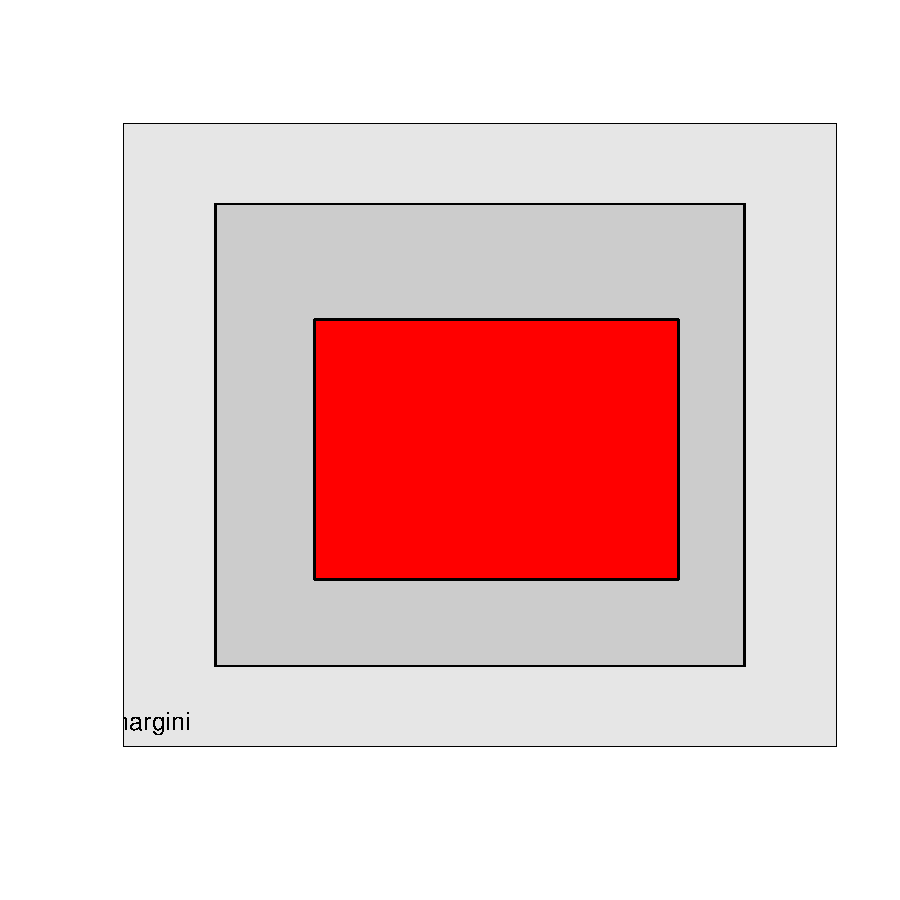
\includegraphics{RbookParte2-259}

Tale modifica si opera con il comando \texttt{mar}.
\begin{equation}\texttt{par}(\texttt{mar=c}(l_1, l_2, l_3, l_4))
\end{equation}
dove $l_1$,$ l_2$, $l_3$,$ l_4$ sono le linee di testo da lasciare libere per annotazioni su ciascun lato come in figura.
Un comando analogo \`e \texttt{mai}, che consente di definire gli spazi in {\it inch} (pollici):
\begin{equation}\texttt{par}(\texttt{mai=c}(i_1, i_2, i_3, i_4))\end{equation}
Infine, \`e possibile definire direttamente la regione di plot utilizzando \texttt{pin}, di sintassi:
\begin{equation*}
\texttt{par(pin=c}(w,h))\end{equation*}
dove $w$ \`e la larghezza e $h$ l'altezza della regione di plot.
Proviamo i comandi:


\begin{Schunk}
\begin{Sinput}
> par(mar=c(1,1,1,1))
> plot(1:10)
> par(mai=c(1,1,1,1))
> plot(1:10)
> par(fin=c(5,3)) ##notare come questa sia centrata
> plot(1:10)
\end{Sinput}
\end{Schunk}
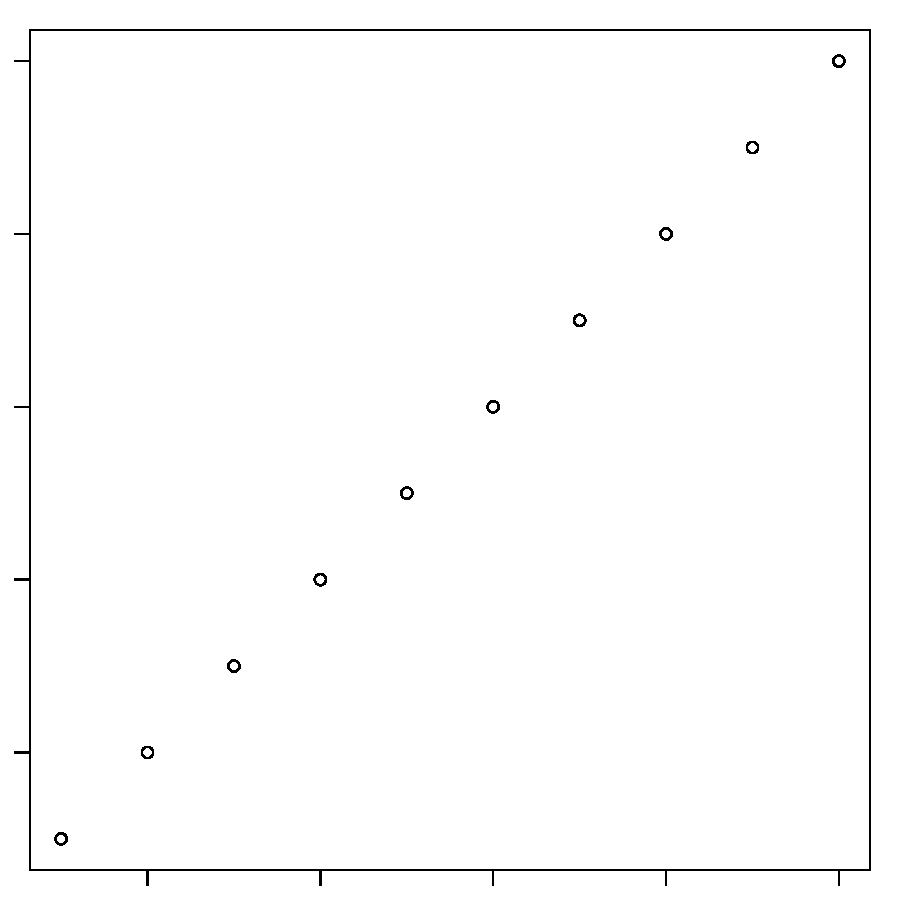
\includegraphics{RbookParte2-260}

\subsection{Il pacchetto  \texttt{lattice}}
Il pacchetto \texttt{lattice} consente di utilizzare funzioni avanzate di grafica, tra cui alcune che sono in grado di lavorare con \emph{data.frame} anche molto complessi.
\subsubsection{Grafica 3D, il vulcano con la grafica non tradizionale del pacchetto \texttt{lattice}}
Una prima funzione in particolare  \`e la funzione \texttt{wireframe}, parente stretta di \texttt{persp3D} e delle funzioni 3D di \texttt{rgl}.
Possiamo utilizzarla per realizzare il plot del solito vulcano, in particolare abilitando la colorazione (\texttt{shade=F} evita  il riempimento), dandone un aspetto pieno (rapporto larghezza/altezza, dipendente da \texttt{ratio}) e definendo una sorgente di luce particolare:
%codechunk
\begin{Schunk}
\begin{Sinput}
> library(datasets)
> library(lattice)
> pdf(file="provawire.pdf")
> wireframe(volcano, shade = TRUE,
+ aspect = c(61/87, 0.4),
+ light.source = c(10,0,10))
> dev.off()
\end{Sinput}
\end{Schunk}

\begin{figure}[htbp]
\begin{center}
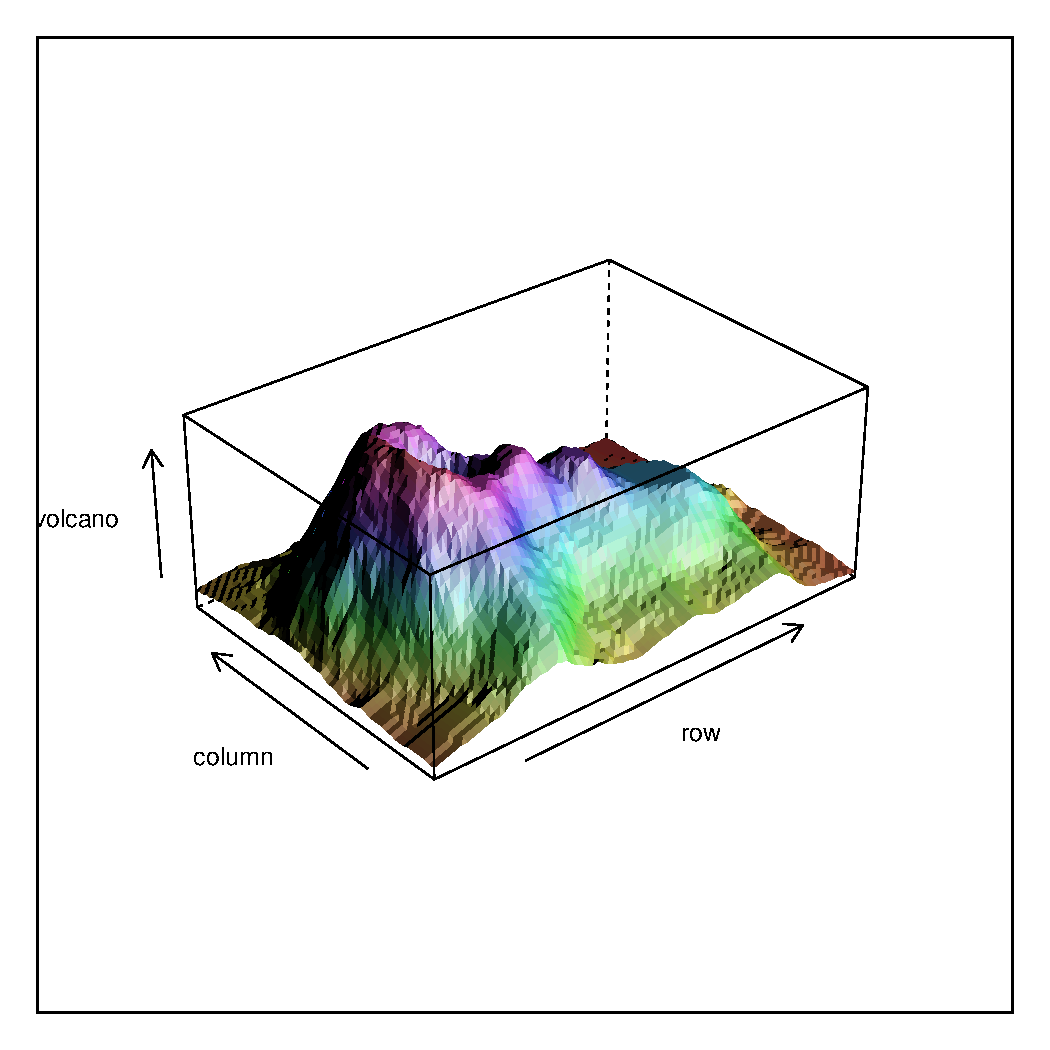
\includegraphics[scale=0.6]{../grafici/wire.pdf}
\caption{Grafico wireframe.}
\label{wirex}
\end{center}
\end{figure}


Una seconda funzione importante, che consente di realizzare dei plot in tre dimensioni \`e \texttt{cloud}.  \index{\texttt{cloud}}
Se ad esempio disponiamo di una tabella come \texttt{Titanic} (riporta il numero di passeggeri sopravvissuti o meno al naufragio ripartiti per et\`a, classe di viaggio e sesso) e voletssimo ottenere invece una tabella che ne riporti la proporzione  sul totale possiamo usare la funzione \texttt{prop.table()}.
Disegnamo ora con \texttt{cloud} la situazione dopo il naufragio, con
\texttt{strip}\index{\texttt{strip}} definiamo le due righe di titolo (in cui sono ripartiti i dati), e con la quadra [,1:2]  finale disegniamo entrambe le classi (sopravvissuti e non sopravvissuti).
\begin{Schunk}
\begin{Sinput}
> pdf(file="../grafici/Titanic.pdf")
> library(lattice)
> cloud(prop.table(Titanic),
+ type = c("p", "h"), strip = strip.custom(strip.names = TRUE),
+ scales = list(arrows = FALSE, distance = 2), panel.aspect = 0.7,
+ zlab = "Proportion")[,1:2]
> dev.off()
\end{Sinput}
\end{Schunk}
\begin{figure}[htbp]
\begin{center}
\includegraphics[scale=0.8]{../grafici/Titanic.pdf}
\caption{default}
\label{defagult}
\end{center}
\end{figure}


Oppure rappresentiamo il \emph{dataset} colore occhi/capelli degli studenti ripartito in base al sesso
\begin{Schunk}
\begin{Sinput}
> pdf(file="../grafici/cloudgraph.pdf")
> library(lattice)
> cloud(prop.table(HairEyeColor),
+ type = c("p", "h"),
+ strip = strip.custom(strip.names = TRUE))
> dev.off()
\end{Sinput}
\begin{Soutput}
pdf 
  2 
\end{Soutput}
\end{Schunk}
\begin{figure}[htbp]
\begin{center}
\includegraphics[scale=0.8]{../grafici/cloudgraph.pdf}
\caption{Cloud graph}
\label{defaulgt}
\end{center}
\end{figure}
\subsection{Il \texttt{parallel plot}}
Un plot di questo tipo parte da una matrice o da un \emph{dataframe}, rappresentando graficamente ogni riga dello stesso (ingresso) con le sue coordinate (il cui numero dipende dal numero dei parametri). I punti ottenuti vengono cos? congiunti da segmenti (attribuendo un colore automatico ad ogni campione, ridefinibile). L'idea di fondo \`e quella di valutare se campioni ad esempio di specie o fenotipi differenti presentano profilo simile (e se diverso lo scopo \`e quello di identificare le variabili/colonne discriminanti).
Nell'esempio vogliamo rappresentare larghezza e lunghezza dei petali e del sepalo dei fiori Iris, volendone poi valutare i profili tra le tre differenti specie. I dati che ci interessano sono cos? le prime 4 colonne (diremo iris[1:4 perch\'e il modello della funzione  lo richiede) mentre le intestazioni saranno le specie di iris, definite da Species, iris.
%code chunk
\begin{Schunk}
\begin{Sinput}
> pdf(file="../grafici/parallelplot.pdf")
> parallelplot(~iris[1:4] | Species, iris)
> dev.off()
\end{Sinput}
\begin{Soutput}
pdf 
  2 
\end{Soutput}
\end{Schunk}
\begin{figure}[htbp]
\begin{center}
\includegraphics[scale=0.6]{../grafici/parallelplot.pdf}
\caption{Cloud graph}
\label{defauglt}
\end{center}
\end{figure}

Oppure valutiamo due diversi trattamenti con vitamina C per la crescita dei denti suini,
ricordate?
%code chunk

\begin{Schunk}
\begin{Sinput}
> library(lattice)
> pdf(file="../grafici/parplot2.pdf")
> parallelplot(~ToothGrowth[c(1,3)] | supp,ToothGrowth)
> dev.off()
\end{Sinput}
\begin{Soutput}
pdf 
  2 
\end{Soutput}
\end{Schunk}
\begin{figure}[htbp]
\begin{center}
\includegraphics[scale=0.6]{../grafici/parplot2.pdf}
\caption{Cloud graph}
\label{defadult}
\end{center}
\end{figure}


\subsection{Applicazione in campo geografico}
Proveremo ora a rappresentare gli Stati Uniti d'America sfruttando un \emph{dataset} predisposto e due nuovi pacchetti che sono spesso utilizzati per studi geografici e rappresentazione di cartine topologiche.  Esse sono in particolare \texttt{sp} ({\it spatial graphs}, con numerosi comandi di grafica) e \texttt{maptools}, che si compone sostanzialmente di funzioni in grado di lavorare con dei poligoni.
Scaricate (dal menu installazione pacchetti) e caricate i due pacchetti:
%code chunks
\begin{Schunk}
\begin{Sinput}
> library(sp)
> library(maptools)
> #gpclibPermitt()
\end{Sinput}
\end{Schunk}
Fatto ci\`o, la prima cosa da fare \`e leggere il contenuto del file {\it sids.shp}, il quale contiene le informazioni sui poligoni (i vari stati componenti),  i confini e le annotazioni letterarie (ad es. file capitali). Il file risiede nelle {\it library} di sistema di \textsf{R} (indirizzo visibile col comando: system.file(-shapes/sids.shp)).
Costruiamo l'oggetto base (\texttt{nc}) e trattiamo le coordinate con CRS:
\begin{Schunk}
\begin{Sinput}
> options(width=55)
> nc <- readShapePoly(system.file("shapes/sids.shp", package="maptools")[1],
+ proj4string=CRS("+proj=longlat +datum=NAD27"))
> names(nc)
\end{Sinput}
\end{Schunk}

Poi creiamo i due pannelli \texttt{pannello1} e \texttt{pannello2} con il comando \texttt{sample} (sceglie un campione di 100 numeri a caso tra 1 a 5), con etichette le prime 5 lettere dell'alfabeto.
\begin{Schunk}
\begin{Sinput}
> set.seed(31) #fissiamo il random seed per il sample
> nc$pannello1 = factor(sample(1:5,100,replace=T),labels=letters[1:5])
> nc$pannello2 = factor(sample(1:5,100,replace=T),labels=letters[1:5])
\end{Sinput}
\end{Schunk}
Ora carichiamo la grafica di \texttt{RColorBrewer}:

\begin{Schunk}
\begin{Sinput}
> library(RColorBrewer)
\end{Sinput}
\end{Schunk}
e utilizziamo \texttt{spplot}, la funzione costruita appositamente per lavorare con dati spaziali aventi
attributi. Essa pendere come ingressi \texttt{nc}, gli attributi f, g e colorer\`a le regioni con la paletta
brewer.pal(5,Set3). Potrete poi provare anche Set1 e Set2.

\begin{Schunk}
\begin{Sinput}
> pdf("../grafici/SPPLOT.pdf")
> spplot(nc, c("pannello1","pannello2"),
+ col.regions=brewer.pal(5, "Set3"), scales=list(draw=TRUE))
> dev.off()
\end{Sinput}
\end{Schunk}
\begin{figure}[htbp]
\begin{center}
\includegraphics[scale=0.6]{../grafici/SPPLOT.pdf}
\caption{maptool}
\label{maptool}
\end{center}
\end{figure}

%\includegraphics{"grafici/mioSPPLOT.pdf"}

\begin{Schunk}
\begin{Sinput}
> library(datasets) #eurodist
> require(stats); require(graphics)
> plot(rate ~ conc, data = Puromycin, las = 1,
+ xlab = "Substrate concentration (ppm)",
+ ylab = "Reaction velocity (counts/min/min)",
+ pch = as.integer(Puromycin$state),
+ col = as.integer(Puromycin$state),
+ main = "Puromycin data and fitted Michaelis-Menten curves")
\end{Sinput}
\end{Schunk}
\includegraphics{RbookParte2-272}

Sarebbe poi meglio sostituire con il reale valore degli anni le etichette presenti sull'asse $x$ originale. Questo si pu\`o ottenere in diversi modi (vedi \texttt{axis}), ma perch\'e non sfruttare l'attributo \texttt{names} della struttura dati?

\begin{Schunk}
\begin{Sinput}
> names(dati)<-as.character(floor(seq(1860,1959,length=length(dati))))
>  plot(as.vector(names(dati)),dati,main="Andamento delle scoperte scientifiche 1860-1959",
+ xlab="Anni, dal 1860 al 1959",ylab="Numero di scoperte",type="o",
+ col="dark green",cex=0.5,lty=4)
\end{Sinput}
\end{Schunk}

Possiamo poi anche orientare diversamente il grafico, scambiando l'asse \texttt{x} con l'asse \texttt{y}, la
rappresentazione dei dati specie nell'insieme pu\`o apparire pi\`u appropriata, oppure peggiore:
%code chunk
\begin{Schunk}
\begin{Sinput}
> plot(dati,as.vector(names(dati)),main="Andamento delle scoperte scientifiche 1860-1959",
+ xlab="Anni, dal 1860 al 1959",ylab="Numero di scoperte",type="o",
+ col="dark green",cex=0.5,lty=4,lwd=2)
\end{Sinput}
\end{Schunk}


\subsection{Il parametro \texttt{las}}
L'orientamento delle etichette degli assi \`e molto importante, il parametro \texttt{las} \index{\texttt{las}} , che assume valori interi tra 0 e 3 pu\`o essere usato a questo scopo. Provate a capire cosa succede al comando precedente aggiungendo nei parametri \texttt{las=2} e altri possibili valori.


\section{I rettangoli}
\textsf{R} consente di disegnare forme (dette primitive) come rettangoli o poligoni. I rettangoli in particolare sono molto utili e versatili, consentendo di realizzare riquadri, evidenziare regioni grafiche, ecc.
\begin{Schunk}
\begin{Sinput}
> plot(c(100, 200), c(300, 450), type= "n", xlab="", ylab="")
> rect(100, 300, 125, 350)
> rect(100, 400, 125, 450, col="green", border="blue")
> rect(115, 375, 150, 425, col=par("bg"), border="transparent")
> rect(150, 300, 175, 350, density=10, border="red")
> rect(150, 400, 175, 450, density=30, col="blue", angle=-30, border="transparent")
> legend(180, 450, legend=1:4, fill=c(NA, "green", par("fg"), "blue"), density=c(NA, NA, 10, 30), angle=c(NA, NA, 30, -30))
\end{Sinput}
\end{Schunk}
\includegraphics{RbookParte2-275}
Ed ora, riproduciamo un Mondrian:
\begin{Schunk}
\begin{Sinput}
> par(bg=rgb(0.95,0.96,0.9))
> plot(NA,xlim=c(0,1),ylim=c(0,1),axes=F,xlab="",ylab="",main="Mondrian Virtuale")
> rect(0,0,1,1,col=rgb(0.95,0.96,0.9),lwd=1)
> rect(0.1,0.35,0.6,0.9,col=rgb(0.973,0.09,0.047),lwd=8)
> rect(0.6,0.625,0.95,0.9,col=rgb(1,0.87,0.34),lwd=8)
> rect(0.6,0.35,0.95,0.625,lwd=8) ##bianco
> rect(0.775,0.35,0.95,0.625,lwd=8) ##bianco 2
> rect(0.6,0.225,0.95,0.35,lwd=8) ##bianco 3
> rect(0.6,0.05,0.95,0.225,lwd=8,col=rgb(0.063,0.008,0.58))
> rect(0.35,0.225,0.6,0.35,lwd=8) #bianco sx 1
> rect(0.35,0.1,0.6,0.225,lwd=8) #bianco sx basso
> rect(0.35,0.05,0.6,0.1,lwd=8,col="black") ##nero sx basso
> rect(0.1,0.1,0.35,0.35,lwd=8,col="black") ##nero sx grande
> rect(0.6,0.908,0.95,1,lwd=NA,col=rgb(1,0.87,0.34)) #giallo alto dx
> rect(0.9575,0,1,0.2,lwd=NA,col=rgb(0.973,0.09,0.047)) #rosso basso dx
> rect(0,0,0.092,0.225,lwd=NA,col=rgb(1,0.87,0.34)) #giallo basso sx
> lines(c(0.02,0.1),c(0.225,0.225),lwd=8,lend="square")
> lines(c(0.02,0.1),c(0.625,0.625),lwd=8,lend="square")
> lines(c(0.02,0.1),c(0.9,0.9),lwd=8,lend="square")
> lines(c(0.2,0.2),c(0.9,0.98),lwd=8,lend="square")
> lines(c(0.95,0.95),c(0.9,0.98),lwd=8,lend="square")
> lines(c(0.6,0.6),c(0.9,0.99),lwd=8,lend="square")
> lines(c(0.95,0.992),c(0.2,0.2),lwd=8,lend="square")
> lines(c(0.95,0.95),c(0.05,0.02),lwd=8,lend="square")
> lines(c(0.35,0.35),c(0.05,0.02),lwd=8,lend="square")
> lines(c(0.1,0.1),c(0.1,0.02),lwd=8,lend="square")
> text(0.45,0.02,"Mondrian Review",cex=0.5)
\end{Sinput}
\end{Schunk}
\includegraphics{RbookParte2-276}

Provate a confrontarlo con l'originale, cercatelo tra le immagini di Google (url{http:/images.google.com})


Il comando  $\texttt{locator}(n)$ \index{\texttt{locator}}
consente di selezionare con il puntatore $n$ punti in un grafico.
Selezioniamo 1 punto cliccando  sul punto che riteniamo il massimo del grafico

\begin{Schunk}
\begin{Sinput}
> locator(1)->coord
\end{Sinput}
\end{Schunk}
 ora clicchiamo sul massimo del grafico

\begin{Schunk}
\begin{Sinput}
> library(datasets)
> plot(as.vector(discoveries))
> coord= c(12,26)
> points(coord[2],coord[1], cex=3, col="red")
\end{Sinput}
\end{Schunk}
\includegraphics{RbookParte2-278}
\section{File Rmd}
\section{ggplot}
\end{comment}
\section*{Tabelle delle distribuzioni statistiche}
Per generare la tabella delle aree sottese dalla distribuzione normale da 0 ad $x$ si deve per prima cosa tenere conto del fatto che \texttt{pnorm}  \`e la cumulativa ad una sola coda. Si sceglie l'intervallo di tabulazione, il numero di colonne ed il numero di cifre.
\begin{Schunk}
\begin{Sinput}
> start=0.01
> stop=3.00
> step=0.01;
> nc=6;
> cifre=5;
> correzione<-function(x)  round(10^cifre* (pnorm(x)-0.5))/10^cifre
>  tabnormale<-cbind(matrix(correzione(seq(start,stop,by=step)),nc=nc),
+  matrix(seq(start,stop,by=step),nc=nc))
> as.vector(t(matrix(c(nc+1:nc,1:nc),nc=2)))->ordinecol
> colnames( tabnormale)= rep(c( "P=A","x"),each=6)
> rownames( tabnormale)=rep("",nrow( tabnormale))
\end{Sinput}
\end{Schunk}
In modo simile per generare la tabella della distribuzione $t$ di Student si selezionano i livelli di fiducia di interesse e  i gradi di libert\`a
%code chunk
\begin{Schunk}
\begin{Sinput}
> gradi=c(1:40,50,60,70,80,90,100,150,200,Inf)
> fiducia=c(0.8,0.85,0.9,0.95,0.98,0.99,0.999);
> ncol=length(fiducia);
> nrow=length(gradi);
> cifre=5;
> tstud<-function(x,gradi,cifre)
+ round(10^cifre*qt((1+x)/2,gradi))/10^cifre
> tabstudent=matrix(0,ncol=ncol,nrow=nrow)
>  for (i in 1:length(fiducia))
+  tabstudent[,i]= tstud(fiducia[i],gradi,5)
>  rownames(tabstudent)=gradi
> colnames(tabstudent)=fiducia
\end{Sinput}
\end{Schunk}
 Per la distribuzione $\chi^2$ si procede esattamente come sopra

\begin{Schunk}
\begin{Sinput}
> gradi=c(1:40,50,60,70,80,90,100,150,200)
> fiducia=c(0.8,0.85,0.9,0.95,0.98,0.99,0.999);
> ncol=length(fiducia);
> nrow=length(gradi);
> cifre=4;
> chiqua<-function(x,gradi,cifre)
+ round(10^cifre*qchisq(x,gradi))/10^cifre
> tabchi=matrix(0,ncol=ncol,nrow=nrow)
> for (i in 1:length(fiducia))
+ tabchi[,i]=chiqua(fiducia[i],gradi,5)
> rownames(tabchi)=gradi
> colnames(tabchi)=fiducia
\end{Sinput}
\end{Schunk}

Per la  distribuzione di Fisher occorre specificare il numero di gradi di libertà del numeratore e del denominatore e fissare i valori di significatività (0.05 e 0.01)

\begin{Schunk}
\begin{Sinput}
> gradinum=1:9
> gradiden=c(1:40,50,60,70,80,90,100,150,200)
> fiducia=c(0.95,0.99);
> ncol=length(gradinum);
> nrow=length(gradiden);
> cifre=3;
> fisher95<-function(gradinum,gradiden,cifre)
+ round(10^cifre*qf(fiducia[1],gradinum,gradiden))/10^cifre
> fisher095=matrix(0,ncol=ncol,nrow=nrow);
> for (i in 1:length(gradinum))
+ fisher095[,i]= fisher95(gradinum[i],gradiden,cifre)
>  rownames(fisher095)=gradiden
> colnames(fisher095)=gradinum
> fisher099=fisher095;
> fisher99<-function(gradinum,gradiden,cifre)
+ round(10^cifre*qf(fiducia
+ [2],gradinum,gradiden))/10^cifre;for (i in 1:length(gradinum))
> fisher099[,i]= fisher99(gradinum[i],gradiden,cifre)
\end{Sinput}
\end{Schunk}
 \setlength\textheight{9in}
\vfill\eject
\section*{Aree $A$  della distribuzione normale da 0 ad $x$}
\oddsidemargin  0.0in
\evensidemargin 0.0in
\topmargin -0.4in
\small
\begin{Schunk}
\begin{Soutput}
    x     P=A    x     P=A    x     P=A    x     P=A    x     P=A    x     P=A
 0.01 0.00399 0.51 0.19497 1.01 0.34375 1.51 0.43448 2.01 0.47778 2.51 0.49396
 0.02 0.00798 0.52 0.19847 1.02 0.34614 1.52 0.43574 2.02 0.47831 2.52 0.49413
 0.03 0.01197 0.53 0.20194 1.03 0.34849 1.53 0.43699 2.03 0.47882 2.53 0.49430
 0.04 0.01595 0.54 0.20540 1.04 0.35083 1.54 0.43822 2.04 0.47932 2.54 0.49446
 0.05 0.01994 0.55 0.20884 1.05 0.35314 1.55 0.43943 2.05 0.47982 2.55 0.49461
 0.06 0.02392 0.56 0.21226 1.06 0.35543 1.56 0.44062 2.06 0.48030 2.56 0.49477
 0.07 0.02790 0.57 0.21566 1.07 0.35769 1.57 0.44179 2.07 0.48077 2.57 0.49492
 0.08 0.03188 0.58 0.21904 1.08 0.35993 1.58 0.44295 2.08 0.48124 2.58 0.49506
 0.09 0.03586 0.59 0.22240 1.09 0.36214 1.59 0.44408 2.09 0.48169 2.59 0.49520
 0.10 0.03983 0.60 0.22575 1.10 0.36433 1.60 0.44520 2.10 0.48214 2.60 0.49534
 0.11 0.04380 0.61 0.22907 1.11 0.36650 1.61 0.44630 2.11 0.48257 2.61 0.49547
 0.12 0.04776 0.62 0.23237 1.12 0.36864 1.62 0.44738 2.12 0.48300 2.62 0.49560
 0.13 0.05172 0.63 0.23565 1.13 0.37076 1.63 0.44845 2.13 0.48341 2.63 0.49573
 0.14 0.05567 0.64 0.23891 1.14 0.37286 1.64 0.44950 2.14 0.48382 2.64 0.49585
 0.15 0.05962 0.65 0.24215 1.15 0.37493 1.65 0.45053 2.15 0.48422 2.65 0.49598
 0.16 0.06356 0.66 0.24537 1.16 0.37698 1.66 0.45154 2.16 0.48461 2.66 0.49609
 0.17 0.06749 0.67 0.24857 1.17 0.37900 1.67 0.45254 2.17 0.48500 2.67 0.49621
 0.18 0.07142 0.68 0.25175 1.18 0.38100 1.68 0.45352 2.18 0.48537 2.68 0.49632
 0.19 0.07535 0.69 0.25490 1.19 0.38298 1.69 0.45449 2.19 0.48574 2.69 0.49643
 0.20 0.07926 0.70 0.25804 1.20 0.38493 1.70 0.45543 2.20 0.48610 2.70 0.49653
 0.21 0.08317 0.71 0.26115 1.21 0.38686 1.71 0.45637 2.21 0.48645 2.71 0.49664
 0.22 0.08706 0.72 0.26424 1.22 0.38877 1.72 0.45728 2.22 0.48679 2.72 0.49674
 0.23 0.09095 0.73 0.26730 1.23 0.39065 1.73 0.45818 2.23 0.48713 2.73 0.49683
 0.24 0.09483 0.74 0.27035 1.24 0.39251 1.74 0.45907 2.24 0.48745 2.74 0.49693
 0.25 0.09871 0.75 0.27337 1.25 0.39435 1.75 0.45994 2.25 0.48778 2.75 0.49702
 0.26 0.10257 0.76 0.27637 1.26 0.39617 1.76 0.46080 2.26 0.48809 2.76 0.49711
 0.27 0.10642 0.77 0.27935 1.27 0.39796 1.77 0.46164 2.27 0.48840 2.77 0.49720
 0.28 0.11026 0.78 0.28230 1.28 0.39973 1.78 0.46246 2.28 0.48870 2.78 0.49728
 0.29 0.11409 0.79 0.28524 1.29 0.40147 1.79 0.46327 2.29 0.48899 2.79 0.49736
 0.30 0.11791 0.80 0.28814 1.30 0.40320 1.80 0.46407 2.30 0.48928 2.80 0.49744
 0.31 0.12172 0.81 0.29103 1.31 0.40490 1.81 0.46485 2.31 0.48956 2.81 0.49752
 0.32 0.12552 0.82 0.29389 1.32 0.40658 1.82 0.46562 2.32 0.48983 2.82 0.49760
 0.33 0.12930 0.83 0.29673 1.33 0.40824 1.83 0.46638 2.33 0.49010 2.83 0.49767
 0.34 0.13307 0.84 0.29955 1.34 0.40988 1.84 0.46712 2.34 0.49036 2.84 0.49774
 0.35 0.13683 0.85 0.30234 1.35 0.41149 1.85 0.46784 2.35 0.49061 2.85 0.49781
 0.36 0.14058 0.86 0.30511 1.36 0.41309 1.86 0.46856 2.36 0.49086 2.86 0.49788
 0.37 0.14431 0.87 0.30785 1.37 0.41466 1.87 0.46926 2.37 0.49111 2.87 0.49795
 0.38 0.14803 0.88 0.31057 1.38 0.41621 1.88 0.46995 2.38 0.49134 2.88 0.49801
 0.39 0.15173 0.89 0.31327 1.39 0.41774 1.89 0.47062 2.39 0.49158 2.89 0.49807
 0.40 0.15542 0.90 0.31594 1.40 0.41924 1.90 0.47128 2.40 0.49180 2.90 0.49813
 0.41 0.15910 0.91 0.31859 1.41 0.42073 1.91 0.47193 2.41 0.49202 2.91 0.49819
 0.42 0.16276 0.92 0.32121 1.42 0.42220 1.92 0.47257 2.42 0.49224 2.92 0.49825
 0.43 0.16640 0.93 0.32381 1.43 0.42364 1.93 0.47320 2.43 0.49245 2.93 0.49831
 0.44 0.17003 0.94 0.32639 1.44 0.42507 1.94 0.47381 2.44 0.49266 2.94 0.49836
 0.45 0.17364 0.95 0.32894 1.45 0.42647 1.95 0.47441 2.45 0.49286 2.95 0.49841
 0.46 0.17724 0.96 0.33147 1.46 0.42785 1.96 0.47500 2.46 0.49305 2.96 0.49846
 0.47 0.18082 0.97 0.33398 1.47 0.42922 1.97 0.47558 2.47 0.49324 2.97 0.49851
 0.48 0.18439 0.98 0.33646 1.48 0.43056 1.98 0.47615 2.48 0.49343 2.98 0.49856
 0.49 0.18793 0.99 0.33891 1.49 0.43189 1.99 0.47670 2.49 0.49361 2.99 0.49861
 0.50 0.19146 1.00 0.34134 1.50 0.43319 2.00 0.47725 2.50 0.49379 3.00 0.49865
\end{Soutput}
\end{Schunk}
\vfill\eject
\section*{Distribuzione di Student}
\oddsidemargin 0.0in
\evensidemargin 0.0in
\topmargin -0.4in
\begin{Schunk}
\begin{Sinput}
>  tabstudent
\end{Sinput}
\begin{Soutput}
        0.8    0.85     0.9     0.95     0.98     0.99     0.999
1   3.07768 4.16530 6.31375 12.70620 31.82052 63.65674 636.61925
2   1.88562 2.28193 2.91999  4.30265  6.96456  9.92484  31.59905
3   1.63774 1.92432 2.35336  3.18245  4.54070  5.84091  12.92398
4   1.53321 1.77819 2.13185  2.77645  3.74695  4.60409   8.61030
5   1.47588 1.69936 2.01505  2.57058  3.36493  4.03214   6.86883
6   1.43976 1.65017 1.94318  2.44691  3.14267  3.70743   5.95882
7   1.41492 1.61659 1.89458  2.36462  2.99795  3.49948   5.40788
8   1.39682 1.59222 1.85955  2.30600  2.89646  3.35539   5.04131
9   1.38303 1.57374 1.83311  2.26216  2.82144  3.24984   4.78091
10  1.37218 1.55924 1.81246  2.22814  2.76377  3.16927   4.58689
11  1.36343 1.54756 1.79588  2.20099  2.71808  3.10581   4.43698
12  1.35622 1.53796 1.78229  2.17881  2.68100  3.05454   4.31779
13  1.35017 1.52992 1.77093  2.16037  2.65031  3.01228   4.22083
14  1.34503 1.52310 1.76131  2.14479  2.62449  2.97684   4.14045
15  1.34061 1.51723 1.75305  2.13145  2.60248  2.94671   4.07277
16  1.33676 1.51213 1.74588  2.11991  2.58349  2.92078   4.01500
17  1.33338 1.50766 1.73961  2.10982  2.56693  2.89823   3.96513
18  1.33039 1.50371 1.73406  2.10092  2.55238  2.87844   3.92165
19  1.32773 1.50019 1.72913  2.09302  2.53948  2.86093   3.88341
20  1.32534 1.49704 1.72472  2.08596  2.52798  2.84534   3.84952
21  1.32319 1.49419 1.72074  2.07961  2.51765  2.83136   3.81928
22  1.32124 1.49162 1.71714  2.07387  2.50832  2.81876   3.79213
23  1.31946 1.48928 1.71387  2.06866  2.49987  2.80734   3.76763
24  1.31784 1.48714 1.71088  2.06390  2.49216  2.79694   3.74540
25  1.31635 1.48517 1.70814  2.05954  2.48511  2.78744   3.72514
26  1.31497 1.48336 1.70562  2.05553  2.47863  2.77871   3.70661
27  1.31370 1.48169 1.70329  2.05183  2.47266  2.77068   3.68959
28  1.31253 1.48014 1.70113  2.04841  2.46714  2.76326   3.67391
29  1.31143 1.47870 1.69913  2.04523  2.46202  2.75639   3.65941
30  1.31042 1.47736 1.69726  2.04227  2.45726  2.75000   3.64596
31  1.30946 1.47611 1.69552  2.03951  2.45282  2.74404   3.63346
32  1.30857 1.47494 1.69389  2.03693  2.44868  2.73848   3.62180
33  1.30774 1.47384 1.69236  2.03452  2.44479  2.73328   3.61091
34  1.30695 1.47281 1.69092  2.03224  2.44115  2.72839   3.60072
35  1.30621 1.47184 1.68957  2.03011  2.43772  2.72381   3.59115
36  1.30551 1.47092 1.68830  2.02809  2.43449  2.71948   3.58215
37  1.30485 1.47005 1.68709  2.02619  2.43145  2.71541   3.57367
38  1.30423 1.46923 1.68595  2.02439  2.42857  2.71156   3.56568
39  1.30364 1.46846 1.68488  2.02269  2.42584  2.70791   3.55812
40  1.30308 1.46772 1.68385  2.02108  2.42326  2.70446   3.55097
50  1.29871 1.46199 1.67591  2.00856  2.40327  2.67779   3.49601
60  1.29582 1.45820 1.67065  2.00030  2.39012  2.66028   3.46020
70  1.29376 1.45550 1.66691  1.99444  2.38081  2.64790   3.43501
80  1.29222 1.45349 1.66412  1.99006  2.37387  2.63869   3.41634
90  1.29103 1.45192 1.66196  1.98667  2.36850  2.63157   3.40194
100 1.29007 1.45067 1.66023  1.98397  2.36422  2.62589   3.39049
150 1.28722 1.44694 1.65508  1.97591  2.35146  2.60900   3.35657
200 1.28580 1.44508 1.65251  1.97190  2.34514  2.60063   3.33984
Inf 1.28155 1.43953 1.64485  1.95996  2.32635  2.57583   3.29053
\end{Soutput}
\end{Schunk}
  \normalsize
\section*{Distribuzione $\chi^2$}
\oddsidemargin 0.0in
\evensidemargin 0.0in
\topmargin -0.4in
\small
\begin{Schunk}
\begin{Sinput}
> tabchi
\end{Sinput}
\begin{Soutput}
          0.8      0.85       0.9      0.95      0.98      0.99     0.999
1     1.64237   2.07225   2.70554   3.84146   5.41189   6.63490  10.82757
2     3.21888   3.79424   4.60517   5.99146   7.82405   9.21034  13.81551
3     4.64163   5.31705   6.25139   7.81473   9.83741  11.34487  16.26624
4     5.98862   6.74488   7.77944   9.48773  11.66784  13.27670  18.46683
5     7.28928   8.11520   9.23636  11.07050  13.38822  15.08627  20.51501
6     8.55806   9.44610  10.64464  12.59159  15.03321  16.81189  22.45774
7     9.80325  10.74790  12.01704  14.06714  16.62242  18.47531  24.32189
8    11.03009  12.02707  13.36157  15.50731  18.16823  20.09024  26.12448
9    12.24215  13.28804  14.68366  16.91898  19.67902  21.66599  27.87716
10   13.44196  14.53394  15.98718  18.30704  21.16077  23.20925  29.58830
11   14.63142  15.76710  17.27501  19.67514  22.61794  24.72497  31.26413
12   15.81199  16.98931  18.54935  21.02607  24.05396  26.21697  32.90949
13   16.98480  18.20198  19.81193  22.36203  25.47151  27.68825  34.52818
14   18.15077  19.40624  21.06414  23.68479  26.87276  29.14124  36.12327
15   19.31066  20.60301  22.30713  24.99579  28.25950  30.57791  37.69730
16   20.46508  21.79306  23.54183  26.29623  29.63318  31.99993  39.25235
17   21.61456  22.97703  24.76904  27.58711  30.99505  33.40866  40.79022
18   22.75955  24.15547  25.98942  28.86930  32.34616  34.80531  42.31240
19   23.90042  25.32885  27.20357  30.14353  33.68743  36.19087  43.82020
20   25.03751  26.49758  28.41198  31.41043  35.01963  37.56623  45.31475
21   26.17110  27.66201  29.61509  32.67057  36.34345  38.93217  46.79704
22   27.30145  28.82245  30.81328  33.92444  37.65950  40.28936  48.26794
23   28.42879  29.97919  32.00690  35.17246  38.96831  41.63840  49.72823
24   29.55332  31.13246  33.19624  36.41503  40.27036  42.97982  51.17860
25   30.67520  32.28249  34.38159  37.65248  41.56607  44.31410  52.61966
26   31.79461  33.42947  35.56317  38.88514  42.85583  45.64168  54.05196
27   32.91169  34.57358  36.74122  40.11327  44.13999  46.96294  55.47602
28   34.02657  35.71499  37.91592  41.33714  45.41885  48.27824  56.89229
29   35.13936  36.85383  39.08747  42.55697  46.69270  49.58788  58.30117
30   36.25019  37.99025  40.25602  43.77297  47.96180  50.89218  59.70306
31   37.35914  39.12437  41.42174  44.98534  49.22640  52.19139  61.09831
32   38.46631  40.25630  42.58475  46.19426  50.48670  53.48577  62.48722
33   39.57179  41.38614  43.74518  47.39988  51.74292  54.77554  63.87010
34   40.67565  42.51399  44.90316  48.60237  52.99524  56.06091  65.24722
35   41.77796  43.63994  46.05879  49.80185  54.24383  57.34207  66.61883
36   42.87880  44.76407  47.21217  50.99846  55.48886  58.61921  67.98517
37   43.97822  45.88645  48.36341  52.19232  56.73047  59.89250  69.34645
38   45.07628  47.00717  49.51258  53.38354  57.96880  61.16209  70.70289
39   46.17303  48.12628  50.65977  54.57223  59.20398  62.42812  72.05466
40   47.26854  49.24385  51.80506  55.75848  60.43613  63.69074  73.40196
50   58.16380  60.34599  63.16712  67.50481  72.61325  76.15389  86.66082
60   68.97207  71.34110  74.39701  79.08194  84.57995  88.37942  99.60723
70   79.71465  82.25535  85.52704  90.53123  96.38754 100.42518 112.31693
80   90.40535  93.10575  96.57820 101.87947 108.06934 112.32879 124.83922
90  101.05372 103.90406 107.56501 113.14527 119.64846 124.11632 137.20835
100 111.66671 114.65882 118.49800 124.34211 131.14168 135.80672 149.44925
150 164.34919 167.96177 172.58121 179.58063 187.67850 193.20769 209.26460
200 216.60878 220.74413 226.02105 233.99427 243.18692 249.44512 267.54053
\end{Soutput}
\end{Schunk}
\normalsize\section*{Tabella della distribuzione di Fisher $95\%$}
\oddsidemargin 0.0in
\evensidemargin 0.0in
\topmargin -0.4in
\small
\begin{Schunk}
\begin{Sinput}
> fisher095
\end{Sinput}
\begin{Soutput}
          1       2       3       4       5       6       7       8       9
1   161.448 199.500 215.707 224.583 230.162 233.986 236.768 238.883 240.543
2    18.513  19.000  19.164  19.247  19.296  19.330  19.353  19.371  19.385
3    10.128   9.552   9.277   9.117   9.013   8.941   8.887   8.845   8.812
4     7.709   6.944   6.591   6.388   6.256   6.163   6.094   6.041   5.999
5     6.608   5.786   5.409   5.192   5.050   4.950   4.876   4.818   4.772
6     5.987   5.143   4.757   4.534   4.387   4.284   4.207   4.147   4.099
7     5.591   4.737   4.347   4.120   3.972   3.866   3.787   3.726   3.677
8     5.318   4.459   4.066   3.838   3.687   3.581   3.500   3.438   3.388
9     5.117   4.256   3.863   3.633   3.482   3.374   3.293   3.230   3.179
10    4.965   4.103   3.708   3.478   3.326   3.217   3.135   3.072   3.020
11    4.844   3.982   3.587   3.357   3.204   3.095   3.012   2.948   2.896
12    4.747   3.885   3.490   3.259   3.106   2.996   2.913   2.849   2.796
13    4.667   3.806   3.411   3.179   3.025   2.915   2.832   2.767   2.714
14    4.600   3.739   3.344   3.112   2.958   2.848   2.764   2.699   2.646
15    4.543   3.682   3.287   3.056   2.901   2.790   2.707   2.641   2.588
16    4.494   3.634   3.239   3.007   2.852   2.741   2.657   2.591   2.538
17    4.451   3.592   3.197   2.965   2.810   2.699   2.614   2.548   2.494
18    4.414   3.555   3.160   2.928   2.773   2.661   2.577   2.510   2.456
19    4.381   3.522   3.127   2.895   2.740   2.628   2.544   2.477   2.423
20    4.351   3.493   3.098   2.866   2.711   2.599   2.514   2.447   2.393
21    4.325   3.467   3.072   2.840   2.685   2.573   2.488   2.420   2.366
22    4.301   3.443   3.049   2.817   2.661   2.549   2.464   2.397   2.342
23    4.279   3.422   3.028   2.796   2.640   2.528   2.442   2.375   2.320
24    4.260   3.403   3.009   2.776   2.621   2.508   2.423   2.355   2.300
25    4.242   3.385   2.991   2.759   2.603   2.490   2.405   2.337   2.282
26    4.225   3.369   2.975   2.743   2.587   2.474   2.388   2.321   2.265
27    4.210   3.354   2.960   2.728   2.572   2.459   2.373   2.305   2.250
28    4.196   3.340   2.947   2.714   2.558   2.445   2.359   2.291   2.236
29    4.183   3.328   2.934   2.701   2.545   2.432   2.346   2.278   2.223
30    4.171   3.316   2.922   2.690   2.534   2.421   2.334   2.266   2.211
31    4.160   3.305   2.911   2.679   2.523   2.409   2.323   2.255   2.199
32    4.149   3.295   2.901   2.668   2.512   2.399   2.313   2.244   2.189
33    4.139   3.285   2.892   2.659   2.503   2.389   2.303   2.235   2.179
34    4.130   3.276   2.883   2.650   2.494   2.380   2.294   2.225   2.170
35    4.121   3.267   2.874   2.641   2.485   2.372   2.285   2.217   2.161
36    4.113   3.259   2.866   2.634   2.477   2.364   2.277   2.209   2.153
37    4.105   3.252   2.859   2.626   2.470   2.356   2.270   2.201   2.145
38    4.098   3.245   2.852   2.619   2.463   2.349   2.262   2.194   2.138
39    4.091   3.238   2.845   2.612   2.456   2.342   2.255   2.187   2.131
40    4.085   3.232   2.839   2.606   2.449   2.336   2.249   2.180   2.124
50    4.034   3.183   2.790   2.557   2.400   2.286   2.199   2.130   2.073
60    4.001   3.150   2.758   2.525   2.368   2.254   2.167   2.097   2.040
70    3.978   3.128   2.736   2.503   2.346   2.231   2.143   2.074   2.017
80    3.960   3.111   2.719   2.486   2.329   2.214   2.126   2.056   1.999
90    3.947   3.098   2.706   2.473   2.316   2.201   2.113   2.043   1.986
100   3.936   3.087   2.696   2.463   2.305   2.191   2.103   2.032   1.975
150   3.904   3.056   2.665   2.432   2.274   2.160   2.071   2.001   1.943
200   3.888   3.041   2.650   2.417   2.259   2.144   2.056   1.985   1.927
\end{Soutput}
\begin{Sinput}
> 
\end{Sinput}
\end{Schunk}
 \vfill
\eject
\section*{Tabella della distribuzione di Fisher $99\%$}
\oddsidemargin 0.0in
\evensidemargin 0.0in
\topmargin -0.4in
\begin{Schunk}
\begin{Sinput}
> fisher099
\end{Sinput}
\begin{Soutput}
           1        2        3        4        5        6        7        8
1   4052.181 4999.500 5403.352 5624.583 5763.650 5858.986 5928.356 5981.070
2     98.503   99.000   99.166   99.249   99.299   99.333   99.356   99.374
3     34.116   30.817   29.457   28.710   28.237   27.911   27.672   27.489
4     21.198   18.000   16.694   15.977   15.522   15.207   14.976   14.799
5     16.258   13.274   12.060   11.392   10.967   10.672   10.456   10.289
6     13.745   10.925    9.780    9.148    8.746    8.466    8.260    8.102
7     12.246    9.547    8.451    7.847    7.460    7.191    6.993    6.840
8     11.259    8.649    7.591    7.006    6.632    6.371    6.178    6.029
9     10.561    8.022    6.992    6.422    6.057    5.802    5.613    5.467
10    10.044    7.559    6.552    5.994    5.636    5.386    5.200    5.057
11     9.646    7.206    6.217    5.668    5.316    5.069    4.886    4.744
12     9.330    6.927    5.953    5.412    5.064    4.821    4.640    4.499
13     9.074    6.701    5.739    5.205    4.862    4.620    4.441    4.302
14     8.862    6.515    5.564    5.035    4.695    4.456    4.278    4.140
15     8.683    6.359    5.417    4.893    4.556    4.318    4.142    4.004
16     8.531    6.226    5.292    4.773    4.437    4.202    4.026    3.890
17     8.400    6.112    5.185    4.669    4.336    4.102    3.927    3.791
18     8.285    6.013    5.092    4.579    4.248    4.015    3.841    3.705
19     8.185    5.926    5.010    4.500    4.171    3.939    3.765    3.631
20     8.096    5.849    4.938    4.431    4.103    3.871    3.699    3.564
21     8.017    5.780    4.874    4.369    4.042    3.812    3.640    3.506
22     7.945    5.719    4.817    4.313    3.988    3.758    3.587    3.453
23     7.881    5.664    4.765    4.264    3.939    3.710    3.539    3.406
24     7.823    5.614    4.718    4.218    3.895    3.667    3.496    3.363
25     7.770    5.568    4.675    4.177    3.855    3.627    3.457    3.324
26     7.721    5.526    4.637    4.140    3.818    3.591    3.421    3.288
27     7.677    5.488    4.601    4.106    3.785    3.558    3.388    3.256
28     7.636    5.453    4.568    4.074    3.754    3.528    3.358    3.226
29     7.598    5.420    4.538    4.045    3.725    3.499    3.330    3.198
30     7.562    5.390    4.510    4.018    3.699    3.473    3.304    3.173
31     7.530    5.362    4.484    3.993    3.675    3.449    3.281    3.149
32     7.499    5.336    4.459    3.969    3.652    3.427    3.258    3.127
33     7.471    5.312    4.437    3.948    3.630    3.406    3.238    3.106
34     7.444    5.289    4.416    3.927    3.611    3.386    3.218    3.087
35     7.419    5.268    4.396    3.908    3.592    3.368    3.200    3.069
36     7.396    5.248    4.377    3.890    3.574    3.351    3.183    3.052
37     7.373    5.229    4.360    3.873    3.558    3.334    3.167    3.036
38     7.353    5.211    4.343    3.858    3.542    3.319    3.152    3.021
39     7.333    5.194    4.327    3.843    3.528    3.305    3.137    3.006
40     7.314    5.179    4.313    3.828    3.514    3.291    3.124    2.993
50     7.171    5.057    4.199    3.720    3.408    3.186    3.020    2.890
60     7.077    4.977    4.126    3.649    3.339    3.119    2.953    2.823
70     7.011    4.922    4.074    3.600    3.291    3.071    2.906    2.777
80     6.963    4.881    4.036    3.563    3.255    3.036    2.871    2.742
90     6.925    4.849    4.007    3.535    3.228    3.009    2.845    2.715
100    6.895    4.824    3.984    3.513    3.206    2.988    2.823    2.694
150    6.807    4.749    3.915    3.447    3.142    2.924    2.761    2.632
200    6.763    4.713    3.881    3.414    3.110    2.893    2.730    2.601
           9
1   6022.473
2     99.388
3     27.345
4     14.659
5     10.158
6      7.976
7      6.719
8      5.911
9      5.351
10     4.942
11     4.632
12     4.388
13     4.191
14     4.030
15     3.895
16     3.780
17     3.682
18     3.597
19     3.523
20     3.457
21     3.398
22     3.346
23     3.299
24     3.256
25     3.217
26     3.182
27     3.149
28     3.120
29     3.092
30     3.067
31     3.043
32     3.021
33     3.000
34     2.981
35     2.963
36     2.946
37     2.930
38     2.915
39     2.901
40     2.888
50     2.785
60     2.718
70     2.672
80     2.637
90     2.611
100    2.590
150    2.528
200    2.497
\end{Soutput}
\end{Schunk}
\vfill
\eject

% \begin{thebibliography}{}
\bibitem[DASL]{dasl}
	{The data and Stories Library). {\url{http://lib.stat.cmu.edu/DASL}} }
\bibitem[Dalgaard]{dalgaard}
	{P.Daalgaard). {\it  Introductory Statistics with R }, {\bf Springer}, }
\bibitem[Snedecor-Cochran]{snedecor}
	{George W. Snedecor , William G. Cochran,Statistical Methods }Iowa State University Press; 8 edition (January 15, 1989)
\bibitem[David]{david}
	{David F. M., (1955), Studies in the History of Probability and Statistics I. Dicing and Gaming (A Note on the History of Probability).} {\it Biometrika Trust}, {\bf 42}, 1--15.
\bibitem[Murrell]{murrell}{Paul Murrell,  {\it R graphics}, Chapman\& Hall/CRC}
\end{thebibliography}	 

 	

Per esempio, consideriamo la serie temporale (oggetto di classe \texttt{ts}) \texttt{discoveries} che mostra l'andamento annuale del numero di scoperte scientifiche. Rappresentiamo graficamente tale serie trascurando  prima e ricordandoci poi della sua struttura  addizionale
\printindex
\vfill\eject
\thispagestyle{empty}\cleardoublepage
 \addcontentsline{toc}{chapter}{Bibliografia}
%\bibliographystyle{babplain}
\bibliographystyle{babplain}
\bibliography{../biblio}
%\pagenumbering{arabic}

\vfill\eject\thispagestyle{empty}\cleardoublepage



\begin{comment}
\begin{thebibliography}{}
\bibliographystyle{plain}
\bibitem[DASL]{dasl}
	{The data and Stories Library). {\url{http://lib.stat.cmu.edu/DASL}} }
\bibitem[Dalgaard]{dalgaard}
	{P.Daalgaard). {\it  Introductory Statistics with R }, {\bf Springer}, }
\bibitem[Snedecor-Cochran]{snedecor}
	{George W. Snedecor , William G. Cochran,Statistical Methods }Iowa State University Press; 8 edition (January 15, 1989)
\bibitem[david]{david}
	{David F. M., (1955), Studies in the History of Probability and Statistics I. Dicing and Gaming (A Note on the History of Probability).} {\it Biometrika Trust}, {\bf 42}, 1--15.
\bibitem[Murrell]{murrell}{Paul Murrell,  {\it R graphics}, Chapman\& Hall/CRC}
\end{thebibliography}
\end{comment}
\printindex
\end{document}
